\documentclass[paper=a4,%
  twoside,%
  BCOR4mm,%
  abstract=true,%
  toc=bibliography,%
  chapterprefix=true,%
%  toc=listof,%
  toc=bibliographynumbered,%
%  toc=listofnumbered,%
  open=right,%
  english,%
  pagesize=pdftex]{scrreprt}
\listfiles

\usepackage[
  backend=biber,
  bibencoding=utf8,
  style=numeric-comp,
  sortcites=true,
  giveninits=true
]{biblatex}
\addbibresource{references.bib}

\usepackage{listings,listings-rust,multicol}
\lstset{
  numbers=left,
  %xleftmargin=2.5em,
  %framexleftmargin=2.5em,
  %frame=tb,
  %stepnumber=1,
  %firstnumber=1,
  numberfirstline=true,
  language=Rust,
  %identifierstyle=,
  %stringstyle=\ttfamily,
  %keywordstyle=\color{OliveGreen},
  %keywordstyle=,
  %showstringspaces=false
}

\usepackage{pgfplots}
\pgfplotsset{compat=1.8}
\usepgfplotslibrary{statistics}

\usepackage{xcolor}
\usepackage[eulerchapternumbers]{template}
\usepackage{blindtext}
\usepackage{graphicx}
\graphicspath{ {./img/} }
\usepackage{todonotes}
\usepackage{algorithm}
\usepackage{amsmath}
\usepackage{amssymb}
\usepackage{url}
\usepackage[shortlabels]{enumitem}
\usepackage{xcolor,realboxes,fancyvrb} % fancyvrb for '\Verb' macro

\definecolor{codegray}{rgb}{0.86,0.86,0.86}

\usepackage[most]{tcolorbox}
\tcbset{
  on line,
  frame code={}
  center title,
  left=0pt,
  right=0pt,
  top=0pt,
  bottom=0pt,
  colback=lightgray,
  colframe=white,
  width=\dimexpr\textwidth\relax,
  enlarge left by=0mm,
  boxsep=4pt,
}

\newtcbox{\code}{enhanced,nobeforeafter,tcbox raise base,top=0mm,bottom=0mm,
right=0mm,left=0mm,boxsep=4pt,fontupper=\fontfamily{Fira Code}\selectfont,
colframe=white,colback=codegray}

\usepackage[printonlyused]{acronym}

% Remove warnings
\usepackage{scrhack}
\usepackage{algpseudocode}
\algblock{Input}{EndInput}
\algnotext{EndInput}
\algblock{Output}{EndOutput}
\algnotext{EndOutput}

\usepackage{luacode} % for 'luacode' environment
\begin{luacode}
  -- the following code employs Lua's powerful "string.gsub" function
  function color_texttt ( s )
    s = string.gsub ( s , "\\texttt%b||", "\\tcbox[on line,boxsep=2pt,left=0pt,right=0pt,top=0pt,bottom=0pt,colback=codegray]{%0}" ) 
    s = string.gsub ( s , "\\texttt%b{}", "\\tcbox[on line,boxsep=2pt,left=0pt,right=0pt,top=0pt,bottom=0pt,colback=codegray]{%0}" ) 
    return s
  end
\end{luacode}
%% Define 2 LaTeX macros to switch operation of Lua function on and off
\newcommand{\ColortextttOn}{\directlua{
   luatexbase.add_to_callback ( "process_input_buffer" , 
   color_texttt, "color_texttt" )}}
\newcommand{\ColortextttOff}{\directlua{
   luatexbase.remove_from_callback ( "process_input_buffer" , 
   "color_texttt" )}}
\AtBeginDocument{\ColortextttOn} % Default: activate the Lua function 


\newcommand{\Desc}[2]{\State \makebox[2em][l]{#1}#2}
\newcommand{\mli}[1]{\mathit{#1}}
\newcommand{\authorname}{Vsevolod Tymofyeyev}
\newcommand{\thesistitle}{Search-based Test Suite Generation for Rust}

\usepackage{varioref}
\usepackage[
  colorlinks=true,
  citecolor={webgreen},
  linkcolor={thesisblue},
  urlcolor={black},
  linktocpage
]{hyperref}
% This package must be declared last
\usepackage{cleveref}
\crefname{lstlisting}{listing}{listings}
\Crefname{lstlisting}{Listing}{Listings}

\begin{document}
\automark[section]{chapter}
\frontmatter
\subject{\normalfont~\\[0.5cm]
  %\includegraphics[width=.75\textwidth]{institute-logo}
  ~\\[1.5cm]
  Master's Thesis in Computer Science}
\title{\normalfont \thesistitle{}}
\author{\authorname{}}
\date{\today}
\publishers{Examiners:\\{Prof. Dr. Gordon Fraser}\\
  {\large (Chair of Software Engineering II)}\\[2ex]
  {Prof. Dr. Christian Hammer}\\
  {\large (Chair of Software Engineering I)}
  }
\lowertitleback{~\\
  \textbf{\authorname{}}:\\
  \emph{\thesistitle{}}\\
  Master's Thesis, University of Passau, 2022.
}
\maketitle

\begin{abstract}
  \blindtext
\end{abstract}
\cleardoublepage
\tableofcontents

\mainmatter% Main Document starts here

\chapter{Introduction}
\label{chap:introduction}
In the programming language world, there are two major sides. There are low-level languages that offer better performance at the expense of security and high-level languages that provide security for programmers through certain constructs such as garbage collection, which lead to runtime overhead. The young programming language Rust tries to combine the good from both. This statically typed language for system programming promises a similarly high performance as C++ while maintaining extended type and memory safety by default. It ensures invariants at compile time, which means that abstractions (so-called zero-cost abstractions) and automatic memory management are not associated with any runtime costs, as is the case with managed languages, for example. Rust prevents (among others) the following common problems: dangling pointers, data races, integer overflow, buffer overflow, and iterator invalidation. Only the integer and buffer overflows are checked at runtime, whereas the buffer overflows can be reduced to static checks using iterators~\cite{Anderson2016}. This symbiosis makes the language particularly attractive to developers, as it has seen a rise in popularity rankings for several years in a row~\cite{StackOverflow2020}. Even the most prominent corporations are considering using Rust in parts of their software. According to Microsoft and Google, 70\% of the bugs found in their software in recent years were due to memory leaks caused by widely used insecure languages such as C and C++~\cite{Microsoft2019MemoryBugs, RustInAndroid}. Microsoft, SpaceX, Google, Amazon AWS, and many other companies have already started experimenting with Rust in their products for increased security~\cite{MicrosoftJoinsRust, AmazonLovesRust, RustInAndroid, GoogleRustFoundation}.

\section{Motivation}
Nevertheless, even the Rust compiler cannot guarantee complete correctness, which means that even when using this language, one still has to write tests for their software. The behavior of software can be checked with the help of tests, for instance, unit tests. Unit tests execute minor parts of a program in isolation. Software testing, however, requires specific input data. In most cases, it's the task of a tester or a developer to write tests manually. This procedure is usually very time-consuming and cost-intensive. A suffciently complex piece of software can have thousands of execution paths driven by different input data. A human can easily overlook some of the execution paths. Moreover, software requirements can change over time, which means that existing test suites may have to be manually modified or, in the worst case, rewritten as a result. Thus, covering all possible execution paths is almost impossible in terms of finances and human work~\cite{Myers2012}. It is assumed that about half of the budget in software projects is spent on testing~\cite{Beizer2003}. Still, developers are often pressed for time (e.g., deadlines on projects) and do not have enough time to test the increasingly complex software despite sophisticated testing tools. This is a big problem because even if some minor bugs only lead to the dissatisfaction of an end-user of a product, some others can cause significant and even health damage~\cite{Myers2012}. For this reason, many approaches have emerged in recent years and decades to automate this process by generating tests from a given software~\cite{McMinn_2004}.

However, testing all possible combinations of input data on a program is primarily impossible, even in an automated way. It would, in most cases, lead to many equivalent tests that do the same procedure repeatedly. To avoid the effort, one tries to find representative input data for the respective equivalence classes to execute paths determined by certain classes of input data as little as possible. To this end, many tools exploit symbolic execution. Thereby the \ac{SUT} is analyzed and executed symbolically. A set of constraints is defined for the input data necessary to achieve a particular goal in the executed code~\cite{Clarke1976}. Practically, however, symbolic execution means many complex algebraic manipulations, especially when object-oriented containers are involved~\cite{Korel1990}. \ac{SBST} is an alternative and very active research field whose main idea is to use metaheuristic search techniques to generate a limited number of tests within an acceptable time that satisfy a test criterion (e.g., high code coverage)~\cite{McMinn_2004}.

Since Rust is considered young as a stable programming language and appeared in version 1.0 in 2015~\cite{Rust10}, there are relatively few options for automatic test generation at the time of writing. These are limited to tools that use symbolic execution to search the possible paths in a given program~\cite{cadar2008klee} or random testing tools. Those tools use the \ac{IR} of LLVM, which the Rust compiler exploits. However, as of this writing, there is no known use of \ac{SBST} for Rust. \ac{SBST} is a combination of automatic test generation and metaheuristic search techniques. This subcategory of \ac{SBSE} resorts to optimization algorithms to solve an NP-hard test generation problem as efficiently and effectively as possible with as much test coverage as possible~\cite{Khari2019}. \ac{SBST} optimizes a solution concerning a particular objective, which could be, e.g., test case prioritization, test suite minimization, or maximization of real-time properties of the \ac{SUT}~\cite{Khari2019}. Search-based techniques for testing have proved to yield good results when applied to programs in other languages, especially Java. In general, a vast majority of such tools has been applied to managed languages since the ideas rely on the ability to use some sort of reflection and instrumentation. Java, for instance, is a mature language that provides both. With Reflection one can load, inspect the structure of the \ac{SUT} at runtime and also run generated tests, which access \ac{SUT} on the fly within the same process. Bytecode is a much simplified representation that Java source code is compiled into. There is good tooling support for Bytecode instrumentation.

In contrast to Java and other managed languages, which are run within virtual machines, Rust's source code is compiled directly into machine executable code. It hardly provides any reflection capabilities, so that both analysis as well as instrumentation of the \ac{SUT} needs to be done during compilation phase, i.e., statically. Another point in which Rust differs strongly not only from managed languages is it's affine type system~\cite{Anderson2016}, which sets strict rules to how variables can be used, that is, they cannot be accessed and passed around freely. This fact not only changes the view on how to design a typical program in Rust. The peculiar restrictions of Rust combined with the idea of ''chaotic mutations'' of tests in SBST pose new challenges to test generation for this language.

\section{Contributions}
With our work, we provide the following contributions:
\begin{itemize}
  \item We adopt and redefine the problem of automatically generating test cases for Rust programs using a \ac{GA}. It is able to evolve an initial set of randomly generated test cases based on their execution feedback and produce a final test suite with a high code coverage. The generated tests take into account the pecularities of Rust's type and generic system, so that even though the test cases are randomly generated and modified during the process, the output is still a valid Rust code.
  \item We implement our approach as a wrapper around the original Rust compiler and hook into different phases of the compiler to execute our logic like extracting points of interest or instrumenting the \ac{SUT}. Rust's in-house build system Cargo allows us to provide a custom Rust compiler wrapper when building a \ac{SUT}. The implementation artifacts and the usage guide is available in a GitHub~\footnote{\url{https://github.com/foxycom/master-thesis}} repository.
  \item We evaluate our \ac{GA}-based approach and compare it to a traditional baseline algorithm for test generation, i.e., random search, to obtain certainty about the correctness of the implementation and any performance gain of our approach over the minimum. We also compare our approach with KLEE, a representative of the common alternative to search-based algorithms, namely \ac{DSE}. The evaluation is conducted using a case study built of 15 open source Rust libraries.
\end{itemize}
All data, as well as the case study, can be found on our GitHub repository.

\section{Structure of the Thesis}
% TODO reword
First, we give an overview over the relevant background on approaches and algorithms that automate tasks in software engineering (\Cref{chap:backgroud}), especially in terms of test generation, which is necessary to understand the concept we build our ideas on. We shall then provide an overview over related work (\Cref{chap:state-of-the-art}), both, regarding test generation with the common approaches as well as test generation specifically for Rust. Then, we introduce the basic concepts of the Rust programming language (\Cref{chap:rust-programming-language}) and what are the pecularities of it in contrast to common programming languages like C++, C\#, or Java. With the language concepts being presented to the reader, we in introduce our \textsc{RustyUnit} tool for automatic test case generation (\Cref{chap:sbst-in-rust}) and provide it's implementation details (\Cref{chap:implementation}). To show the performance of our approach, we provide an extensive evaluation (\Cref{chap:evaluation}), followed by an outlook on possible future research directions (\Cref{chap:future-work}).

\clearpage

\chapter{Background}
\label{chap:backgroud}
\section{Test Generation in General}
%Testsgenerierung ist ein aktiv erforschtes Feld in der Wissenschaft. Im Idealfall kann für ein Programm eine Testsuite von Unit Tests generiert werden, die alle möglichen Pfade im \ac{SUT} abdecken und gleichzeitig die Korrektheit der Ausführung jedes einzelnen Pfades durch automatische Orakel überprüft, beispielsweise durch Assertions. Ein Orakel ist ein Mechanismus zum Überprüfen, ob ein Output bei einem gegebenen Input richtig ist, beispielsweise mit Hilfe einer formalen Spezifikation~\cite{McMinn2009}. Leider ist das oft nicht möglich. Zum einen können in einem Programm Ausführungspfade existieren, die schlicht unter keinen Umständen erreicht werden können. Zum anderen hat Software nur sehr selten eine formale Spezifikation, die bei der Generierung verwendet werden kann, um Orakel zu generieren. Somit muss in den meisten Fällen ein Entwickler bzw. Tester die generierte Testsuite manuell mit Orakeln versehen (dazu muss er/sie natürlich selbst wissen was das richtige Verhalten ist)~\cite{Fraser_2013}. Dazu muss die generierte Testsuite aber auch möglichst klein und für den Menschen verständlich gehalten werden.

Test generation is an actively researched field in science. Ideally, a test suite of unit tests can be generated for a program that covers all defined coverage criteria in the \ac{SUT} while checking the correctness of the program by implementing automatic oracles, such as assertions, for the execution of each unit. An oracle is a mechanism for checking whether an output is correct given an input, for example using a formal specification~\cite{McMinn2009}. Unfortunately, this is often not possible. For one thing, execution paths may exist in a program that simply cannot be achieved under any circumstances. For another, software very rarely has a formal specification that can be used for the purpose of generating test cases. Thus, in most cases, a developer or tester must manually add oracles to the generated test suite (for this, of course, they must know what the correct behavior is)~\cite{Fraser_2013}. For this, however, the generated test suite must also be kept as small as possible and understandable for humans.

%Bei einer Testgenerierung wird das Coverage-Kriterium oft als eine Leitlinie benutzt~\cite{Fraser_2011a}. Ein Coverage-Kriterium ist eine Sammlung von Test-Zielen, die typischerweise eins nach dem anderen abgearbeitet bzw. abgedeckt werden, wobei die notwendigen Input-Daten beispielsweise symbolisch oder such-basiert ermittelt werden. Eine beliebte Art des Coverage-Kriteriums ist die Branch-Coverage.

Automatic test generation approaches often exploit some coverage criterion as a guideline~\cite{Fraser_2011a}. A coverage criterion is a collection of test objectives that are typically worked through or covered one at a time, with the necessary input data determined randomly, symbolically, or search-based, for instance. Common types of coverage criteria are branch coverage, mutation coverage, or error coverage. Branches can be arms of an if expression or a loop header. They are executed when a given boolean expression evaluates to \texttt{true} or \texttt{false}. Branches can also be nested, and to find suitable values to reach a (nested) branch, symbolic execution or it's dynamic extension with concrete values can be used. It builds a path that can be resolved by concrete values (if such exist and the path is reachable at all) using a \ac{SMT} solver. An alternative to symbolic execution is a meta-heuristic search. TODO Beschreibung der Coverage-Kriterien?

% Fraser und Arcuri~\cite{Fraser_2011a} listen ein paar verwante Paper dazu auf.

\section{Random Search}
Random search is a baseline strategy that does not rely on recombination, mutation or selection, but on the replacement of existing solutions. The idea is to repeatedly sample new solutions from the search space at random, replacing a previous solution with the new one if the new solution is better with respect to some predefined coverage criterion. Random search can make use of an archive by employing a specific sampling strategy~\cite{Campos2017}. TODO Was ist ein Archiv?

Random testing is a variant of random search, which builds test suites incrementally. With random testing, the program is executed with random inputs, and the executed structures of the program are observed. Individual test cases are sampled from the search space, and if a test case increases the overall coverage of the test suite, it is kept and otherwise discarded~\cite{Campos2017}. Since the landscape of fitness values in generating unit tests is fairly flat and this is a relatively simple search problem, random search can be at least as effective as evolutionary algorithms and sometimes even better~\cite{Shamshiri2015a}.

\section{Symbolic Execution}
Symbolic execution is not an execution of a program in a direct sense. Instead, it assigns symbolic expressions to program variables while tracing a path statically in the program structure~\cite{McMinn_2004}. Ideally, symbolic execution of such a path~$p$ yields a logical formula~$\phi_{p}$, a \textit{path-condition}, describing a set of input data~$I$ for the \ac{SUT} necessary to execute the program~$P$ and follow the path~$p$. An \ac{ATP} determines whether a given path is feasible~\cite{Clarke1976,King1976}. If the formula~$\phi_{p}$ is unsatisfiable, ~$I$ is empty, and the path~$p$ is not feasible. Otherwise, the formula is satisfiable, which results in the set~$I$ being nonempty, and the path~$\phi_{p}$ being feasible~\cite{Ball2015}. In such a case, a model of~$\phi_{p}$ can provide an example~$i \in I$ that can be used in a test to cover the path~$p$. Symbolic execution is a common approach to generate input data or entire unit tests. Many of the tools follow the same principle: instead of running programs with manual or generated input data, the data is populated with symbolic values that can be ''anything'' initially~\cite{cadar2008klee}. Concrete operations on data are replaced by those that can manipulate the symbolic ones. When the execution of the program branches, the tools keep track of the execution of both branches. For each branch, a collection of constraints is stored that must apply to execute that path. If execution ends in a path or the program crashes, a test can be generated from it by using concrete values as input data that satisfy the corresponding path constraints. If the program remains deterministic and unchanged, an execution with concrete input data leads to the same bug in the program. TODO ein grafisches einfaches Beispiel mit mehreren Branches und Formulas darstellen.

%Dynamische symbolische Ausführung ist eine Erweiterung von symbolischer Ausführung, die erlaubt, mit Hilfe einer Kombination aus konkreten und symbolischen Werten eine Reihe von Problemen zu überwinden~\cite{Fraser_2013}. Es gibt eine Reihe von Tools, die für eine automatische Generierung von Tests auf DSE setzen, zum Beispiel CUTE and jCUTE~\cite{Sen2006} und KLEE~\cite{cadar2008klee}. KLEE hat zwei Ziele: (1) das Tool versucht, jede ausführbare Zeile in einem Programm auszuführen, d. h. hohe Statement Coverage zu erreichen und (2) bei jeder gefährlichen Operation (z. B. dereference, assertion) wird versucht zu überprüfen, ob es Werte gibt, die dabei zu einem Fehler führen könnten. Das letztere wird durch symbolische Ausführung erreicht. Da selbst in einfachen Programmen die Anzahl von Ausführungszuständen / -pfaden explodieren kann, wird von KLEE eine Reihe von Heuristiken und Optimisierungstechniken angewendet, um die Performanz zu erhöhen. Zum Beispiel werden nicht ganze Bäume bei Verzweigungen gecloned (Zustände sind nämlich Bäume), sondern es wird der write-on-copy Ansatz auf Objekt-Level angewendet. Unveränderte Teilbäume können von mehreren verschiedenen Zuständen referenziert werden. Außerdem wird versucht, Anfragen an den SAT Solver, um symbolische Werte in konkrete umzuwandeln, so weit vereinfacht wie möglich, da die Verarbeitungszeit der Anfragen alles andere dominiert. Auf diese Weise konnten die Autoren die Ausführungszeit des Tools auf den GNU Coreutils um das 15-fache beschleunigen.

\ac{DSE} is an extension of path-based symbolic execution that allows a combination of concrete and symbolic values to overcome many problems~\cite{Fraser_2013}. Because of the combination of concrete and symbolic values, \ac{DSE} is also called concolic execution. The approach starts by executing a program~$P$ on some input~$i$, seeding the symbolic execution process with a feasible path~\cite{Gupta2000,Korel1992}. Then, \ac{DSE} uses concrete values from the execution~$P(i)$ in place of symbolic expressions whenever symbolic reasoning is not possible or desired~\cite{Cadar2005}. Examples include non-linear arithmetic or cryptographic hash functions that are virtually impossible to solve for symbolic execution~\cite{Ball2015}. Several tools rely on \ac{DSE} for automatic generation of tests, for example, \textsc{KLEE}~\cite{cadar2008klee}, \textsc{CUTE} and \textsc{jCUTE}~\cite{Sen2006}, \textsc{DART}~\cite{Godefroid_2005}, and \textsc{KLOVER}~\cite{Li2011}. 

\section{Evolutionary algorithms}
%Der potenzielle Suchraum für mögliche Inputdaten selbst bei einem sehr simplen Programm kann unendlich groß sein. Metaheuristische Ansätze versprechen eine Abhilfe. Das sind keine geschlossenen Algorithmen an sich, sondern Strategien, die auf spezifische Probleme angepasst werden können. Zum Beispiel wird für die Generierung von Testdaten bei Test Cases eine problem-spezifische Fitnessfunktion definiert, mit deren Hilfe die Qualität möglicher Lösungen des Problems verglichen werden kann~\cite{McMinn_2004}. Metaheurische Suche wird nicht nur für Testdatengenerierung verwendet. Andere Verwendungen umfassen:
The potential search space for possible input data even for a very simple program can be infinite. \acp{EA}, which are metaheuristic approaches, promise a cure. These are not closed algorithms per se, but strategies that can be adapted to specific problems. For example, for test case data generation, a problem-specific fitness function can be defined to compare the quality of possible solutions, i.e., test cases, to the problem~\cite{McMinn_2004}. However, metaheuristic search is not only used for test data generation. Other uses include:
\begin{itemize}
	\item coverage of the program structure as part of a white-box testing strategy,
	\item evaluating a specific program feature according to its formal specification,
	\item attempts to automatically invoke error conditions or breaks of assertions in a program,
	\item verification of non-functional features, for example finding worst-case execution time of a real time system.
\end{itemize}
TODO Links zu einzelnen Paper einfügen, z. B. Automotive.

%Evolutionary algorithms setzen auf simulierte Evolution bei der Suche nach Lösungen zu einem spezifischen Problem und evolvieren Lösungskandidaten mit Hilfe von speziellen Operatoren, die von Genetik und natürlicher Selektion inspiriert sind. Genetische Algorithmen sind die bekannteste Ausprägung der evolutionären Algorithmen und nehmen ihre Anfänge irgendwo her. \todo{Keine Ahnung, ob das überhaupt sinnvoll ist, die Geschichte davon aufzuschreiben.} Eine Suche mit genetischen Algorithmen wird auf Basis von Rekombination von Zwischenlösungen durchgeführt, einem Mechanismus, um Informationen zwischen Lösungen auszutauschen und somit neue züchten~\cite{McMinn_2004}.

Evolutionary algorithms are inspired by natural evolution and have been successfully used to address many kinds of optimization problems. In this context, a solution is encoded ''genetically'' as an individual and a set of individuals is called a population. The population is gradually improved or optimized by performing nature-inspired operations on individuals, such as mutation, which independently changes components of an individual with a low probability, or crossover, which merges at least two individuals to produce offspring~\cite{Campos2017a}. Genetic algorithms are the best known instance of evolutionary algorithms and take their beginnings from \textbf{somewhere}. A search using genetic algorithms is performed based on recombination of intermediate solutions, a mechanism to exchange information between solutions and thus breed new ones~\cite{McMinn_2004}.

\section{Genetic Algorithms}
TODO McMinn hat eine super Beschreibung von genetischen und evolutionären Algorithmen, Selektion, Crossover, Mutation, fortgeschrittene Repräsentationen von Individuen~\cite{McMinn_2004}. Außerdem wird der genetische Algorithmus in \cite{Fraser2011} und \cite{Fraser_2013} beschrieben. \cite{Fraser_2013} beschreibt außerdem die Suchoperatoren.

%TODO In seinem Paper beschreibt Harman~\cite{Harman2002}, wie bestimmte Variablen innerhalb von Verzweigungsknoten bei der Suche rausgefiltert werden können, weil sie keinen Einfluss auf die Branch Distance haben. Somit wird der Suchraum verkleinert.

%Genetische Algorithmen sind die meist verbreitete Form von evolutionären Algorithmen, da sie einfach zu implementieren sind und im Schnitt gute Ergebnisse erzielen. Der Name ''genetischer Algorithmus'' kommt von der Analogie zwischen dem Enkodieren eines Lösungskandidaten als eine Sequenz von simplen Komponenten und der genetischen Struktur eines Chromosomes. Diese Analogie wird fortgeführt, indem einzelne Lösungen als Individuen oder Chromosomen bezeichnet werden~\cite{Campos2017}. Demnach werden Komponenten einer Lösung Gene genannt, wobei mögliche Werte einer Komponente Alleles und ihre Position in der Sequenz Locus heißen. Des Weiteren wird eine tatsächliche enkodierte Repräsentation einer Lösung, die von einem genetischen Algorithmus manipuliert wird, Genotyp und eine dekodierte - Phenotyp genannt~\cite{McMinn_2004}. Algorithm~\labelcref{alg:genetic-algorithm} zeigt abstrakt die Funktionsweise eines Standard genetischen Algorithmus. Die initiale Population wird typischerweise zufällig generiert oder aus einem bestimmten Seed generiert. In folgenden Generationen werden Nachkommen mittels Optimisierungs- oder Suchoperatoren gezüchtet, also Rekombination und Mutation. Es gibt viele Variationen des Standard GA. Zum Beispiel werden bei der monotonen Variante des Standard GA nach der Mutation und Evaluation der Fitness der Nachkommen entweder die besten Nachkommen oder die besten ''Parents'' der nächsten Population hinzugefügt. Beim Standard GA werden an der Stelle sowohl ''Parents'' als auch Nachkommen der nächsten Population hinzugefügt. Eine weitere Variante von Standard GA ist der Steady State GA, der wie die monotone Variante nur die besten Individuen nach einer Mutation behält, jedoch anstatt eine neue Population von Nachkommen zu kreieren, ersetzt die ''Parents'' durch Nachkommen in der ursprünglichen Population~\cite{Campos2017}.

Genetic algorithms are the most common form of evolutionary algorithms because they are easy to implement and produce good results on average. The name ''genetic algorithm'' comes from the analogy between encoding a candidate solution as a sequence of simple components and the genetic structure of a chromosome. This analogy is continued by calling individual solutions individuals or chromosomes~\cite{Campos2017}. Accordingly, components of a solution are called genes, with possible values of a component called alleles and their positions in the sequence called locus. Furthermore, an actual encoded representation of a solution manipulated by a genetic algorithm is called genotype and a decoded one phenotype~\cite{McMinn_2004}. \Cref{alg:genetic-algorithm} abstractly shows the mechanism of a standard genetic algorithm. The initial population of size~$p_s$ of candidate solutions is typically randomly generated or generated from a particular seed. Afterwards, a pair of individuals is selected from the population using some selection algorithm~$s_f$, such as rank-based, elitism, or tournament selection. Next, both selected individuals are recombined using crossover~$c_f$, e.g., single point or multiple point crossover, with a probability~$c_p$ to produce two new offspring $o_1$, $o_2$. Then, mutation is applied on both offspring, independently changing the genes with a probability of $m_p$, which usually is equal to $\frac{1}{n}$, where $n$ is the number of genes in a chromosome. The two mutated offspring are then included in the next population. At the end of each iteration, the fitness value of all individuals is computed.  

There are many variations of standard \ac{GA}. For example, in the monotonic variation of standard \ac{GA}, after mutation and evaluation of the fitness of the offspring, either the best descendants or the best parent chromosomes are added to the next population. In standard \ac{GA}, both parents and descendants of the next population are added at this point. Another variant of standard algorithm is steady state \ac{GA}, which, like the monotonic variant, retains only the best individuals after a mutation, but instead of creating a new population of offspring, replaces the ''parents'' with offspring in the original population~\cite{Campos2017}.

%Die unter anderem wesentlichen Punkte beim \Cref{alg:genetic-algorithm} sind das Messen der Fitness eines einzelnen Tests und der Mutationsoperator oder -funktion. Diese sind Faktoren, mit deren Hilfe eine aktuelle Population zu einer neuen evolviert werden, die mehr Chancen hat, einen Target abzudecken. Die Fitness bestimmt eines Individuums, zu überleben und in der neuen Population, evtl. in einer mutierten Form, teilzunehmen. Ein Mutationsoperator bestimmt hingegen, auf welche Weise neue Individuen (Test Cases) aus gegebenen generiert werden~\cite{Tonella2004}. Die Selektion von Individuen wird durch Fitness Funktionen gesteuert, sodass Individuen mit guter Fitness mit höher Wahrscheinlichkeit überleben und in der Zucht von Nachkommen teilnehmen. Im Kontext von Testgenerierung basieren Fitness Funktionen auf Kriterien der Code Coverage, wie z. B. Statement oder Branch Coverage. In den letzten Jahren gab es einen Trend, die Suche nach mehreren Coverage Kriterien gleichzeitig zu optimieren. Da Coverage Kriterien typischerweise keine widersprüchliche Ziele darstellen, können diese in einer weigted linearen Funktion kombiniert werden~\cite{Rojas2015}. Eine hohe Anzahl von Coverage Zielen kann jedoch die Performanz eines evolutionären Algorithmus negativ beeinflussen. Um das zu vermeiden, können generierte Tests für abgedeckte Ziele in einem Archiv gespeichert werden~\cite{Rojas2017}, wobei die Fitness Funktion dynamisch adaptiert wird, um die Suche nur in Richtung nicht abgedeckter Ziele zu leiten. Der Archiv kann auch bei für bessere Effektivität von Suchoperatoren verwendet werden, in dem beispielsweise neue Tests durch Mutation von bestehenden aus dem Archiv und nicht zufällig generiert werden~\cite{Campos2017}.

The essential points in the \Cref{alg:genetic-algorithm} are measuring the fitness of a single chromosome and the mutation operator. These are factors that help to evolve a current population into a new one that has more chances to cover a coverage criterion. Fitness determines an individual's ability to survive and participate in the new population, possibly in a mutated form. A mutation operator, on the other hand, determines the way in which new individuals are generated from given ones~\cite{Tonella2004}. Selection of individuals is controlled by fitness functions, so that individuals with good fitness are more likely to survive and participate in breeding offspring. In the literature about search-based test generation, fitness functions are commonly defined as some code coverage criteria, e.g., statement or branch coverage. In recent years, there has been a trend to optimize searches for multiple coverage criteria simultaneously. Since coverage criteria typically do not represent conflicting goals, they can be combined in a weigted linear function~\cite{Rojas2015}. However, a high number of coverage goals can negatively affect the performance of an evolutionary algorithm. To avoid this, generated tests for covered targets can be stored in an archive~\cite{Rojas2017}, where the fitness function is dynamically adapted to guide the search only towards uncovered targets. The archive can also be used in for better effectiveness of search operators, in which, for example, new tests are generated by mutating existing ones from the archive rather than randomly~\cite{Campos2017}.

\begin{algorithm}
\caption{A high level description of a standard genetic algorithm~\cite{Campos2017}}\label{alg:genetic-algorithm}
\begin{algorithmic}
\Input
  \Desc{$C$}{Stopping condition}
  \Desc{$\delta$}{Fitness function}
  \Desc{$p_s$}{Population size}
  \Desc{$s_f$}{Selection function}
  \Desc{$c_f$}{Crossover function}
  \Desc{$c_p$}{Crossover probability}
  \Desc{$m_f$}{Mutation function}
  \Desc{$m_p$}{Mutation probability}
  \EndInput
  \Output
  \Desc{$P$}{Population of optimized individuals}
  \EndOutput
\State $P \gets GenerateRandomPopulation(p_s)$
\State $PerformFitnessEvaluation(\delta, P)$

\While{$\neg C$}
    \State $N_P \gets \{\}$
    \While{$\left| N_P \right| < p_s$}
        \State $p_1, p_2 \gets Selection(s_f, P)$
        \State $o_1, o_2 \gets Crossover(c_s, c_p, p_1, p_2)$
        \State $Mutation(m_f, m_p, o_1)$
        \State $Mutation(m_f, m_p, o_2)$
        \State $N_P \gets N_P \cup \{o_1, o_2\}$
    \EndWhile
    \State $P \gets N_P$
    \State $PerformFitnessEvaluation(\delta, P)$
\EndWhile
\State \Return $P$
\end{algorithmic}
\end{algorithm}

\subsection{Crossover}
\label{sec:background-crossover}
%Ein wesentlicher Teil von genetischen Algorithmen ist die sogenannte Rekombination oder auch Crossover. Dieser Operator nimmt zwei Parent-Lösungen als Input und verbindet sie in einer bestimmten Weise, um zwei Nachkommen-Lösungen zu produzieren. Es gibt viele verschiedene Arten von Rekombination, aber die einfachste ist die One-Point-Rekombination~\cite{McMinn_2004}. Dabei wird ein einzelner Punkt in den zwei Lösungssequenzen gewählt, der die Sequenzen in Kopf und Schwanz trennt. Die Köpfe bzw. die Schwänze werden dann zwischen den beiden Sequenzen ausgetauscht. Eine One-Point Rekombination von zwei Individuen $[0, 255, 0]$ und $[255, 0, 255]$, die in Binärform jeweils als $000000001111111100000000$ und $111111110000000011111111$ enkodiert wären, an der Stelle $12$ würde zu folgenden zwei Nachkommen führen~\cite{McMinn_2004}:
An essential part of genetic algorithms is the so-called recombination or crossover. This operator loosely models the exchange of genetic information that takes place during reproduction in the natural world. This operator takes two or more parent solutions as input and combines them in a certain way to produce two or mroe offspring solutions. There are many different types of recombination, but the simplest one is one-point recombination~\cite{McMinn_2004}. It involves choosing a single point in two solution sequences that separates the sequences into heads and tails. The heads or tails are then exchanged between the  sequences. A one-point recombination of two individuals $[0, 255, 0]$ and $[255, 0, 255]$, which would be encoded in binary as $0000000011111100000000$ and $111111110000111111$, respectively, at position $12$ would result in the following two offspring~\cite{McMinn_2004}:

\[
\left.\begin{array}{c}
\textcolor{webgreen}{000000001111} \\  %
\textcolor{thesisblue}{111111110000} %
\end{array}\right|
\begin{array}{c}
\textcolor{webgreen}{111100000000} \\  %
\textcolor{thesisblue}{000011111111} %
\end{array} \longrightarrow
\begin{array}{c}
\textcolor{webgreen}{000000001111}\textcolor{thesisblue}{000011111111} \\  %
\textcolor{thesisblue}{111111110000}\textcolor{webgreen}{111100000000} %
\end{array}
\]


\subsection{Selection}
%Es können viele verschiedene Selektionsmechanismen angewendet werden, um zu entscheiden, welche Individuen für eine Nachkommenschaft herangezogen werden sollen. Der Fokus liegt dabei auf der Fitness der Individuen. Der Fitnesswert kann dabei entweder direkt verwendet oder erst auf eine bestimmte Weise skaliert werden.

%Genetische Algorithmen speichern eine ganze Population von Lösungen, statt nur einer aktuellen Lösung. Das hilft vor allem initial mehr vom Suchraum zu sampeln, indem mehrere Startpunkte definiert werden. Die Population wird iterativ rekombiniert und mutiert, um weitere Populationen durch das Evolvieren zu züchten, die als Generationen bekannt sind. Die Idee einer Rekombination besteht darin, fittere Individuen vorzuziehen, in der Hoffnung, dadurch auch fittere Nachkommen zu züchten. Jedoch kann eine viel zu sehr fokusierte Selektion auf am meisten fitte Individuen dazu führen, dass diese die die nächsten Generationen dominieren werden und so aufgrund niederiger Diversität die Suche nur auf einen bestimmten Bereich im Suchraum begrenzen. Auf der anderen Hand, eine zu schwache Selektion kann dazu führen, dass die Suche in einer viel zu breiten Exploration des Suchraumes endet, wodurch kein signifikanter Fortschritt in Richtung optimaler Lösung geschafft wird~\cite{McMinn_2004}.

%Der originale Selektionsalgorithmus von Holland~\cite{Holland1992} setzte auf \textit{Fitness-proportionale Selektion}. Dieser Selektionsmechanismus wies jedem Individuum, wie oft es für Reproduktion ausgewählt wird, basierend auf der Fitness des jeweiligen Individuums im Vergleich zum Rest der Population. Der Prozess ist analog zu einer Roulettescheibe: Jedem Individuum wird ein Abschnitt auf der Scheibe entsprechend seinem Fitnesswert zugewiesen. Die Scheibe wird dann $N$ mal gedreht, um $N$ ''Eltern'' auszuwählen. Am ende jeder Runde bestimmt die Position des Markers auf der Scheibe das Individuum, das als ''Parent'' für die nächste Generation ausgewählt wurde. Fitness-proportionale Selektion kann aber zu Schwierigkeiten führen, eine konstante Selection Pressure zu halten. Selection Pressure ist die Wahrscheinlichkeit, dass das beste Individuum ausgewählt wird im Vergleich zur durchschnittlichen Wahrscheinlichkeit aller Individuen, ausgewählt zu werden. In den ersten Generationen einer Suche die Varianz von Fitnesswerten einer Population ist typischerweise hoch, was dazu führt, dass auch die Selection Pressure einer Fitness-proportionalen Selektion hoch ist. Das kann zu einer viel zu früher Konvergenz führen. In den späteren Generationen, wenn sich die Fitnesswerte von Individuen nicht mehr so stark unterscheiden, fällt die Selection Pressure ab, was zur Stagnation bei der Suche führen kann.

%Sobald die Sammlung von ''Parents'' ausgewählt wurde, wird die Rekombination angewendet, um die nächste Generation zu züchten. Crossover wird auf die ausgewählten Individuen mit der Wahrscheinlichkeit $p_c$ angewendet. $p_c$ wird auch als Crossover rate oder Crossover probability bezeichnet. Falls Crossover angewendet wird, werden die neuen Nachkommen der neuen Population hinzugefügt. Ansonsten werden die selektierten ''Parents'' unverändert in die neue Population kopiert. Nach diesem Schritt wird die Mutationsphase eingeleitet, die für das Einführen bzw. Wiedereinführen eines neuen genetischen ''Materials'' verantwortlich ist, welcher Diversität der Suche erhöhen soll.

Many different selection mechanisms can be used to decide which individuals should be used for a breed. The focus is on the fitness of the individuals. A fitness value can either be used directly or scaled in a certain way first.

Genetic algorithms store a whole population of solutions instead of only one current solution. This primarily helps to initially sample more of the search space by defining multiple starting points. The population is iteratively recombined and mutated to breed further populations through evolving, known as generations. The idea of recombination is to prefer fitter individuals in the hope of breeding fitter offspring. However, too focused selection on the most fit individuals can lead to them dominating the next generations and thus limiting the search to only a certain area in the search space due to low diversity. On the other hand, too weak selection may result in a search that is far too broad in its exploration of the search space, thus failing to make significant progress toward an optimal solution~\cite{McMinn_2004}.

Holland's original selection algorithm~\cite{Holland1992} relied on \textit{fitness-proportional selection}. This selection mechanism assigned to each individual how often it would be selected for reproduction based on the fitness of that individual relative to the rest of the population. The process is analogous to a roulette wheel: each individual is assigned a section on the wheel according to its fitness value. The disk is then spun $N$ times to select $N$ ''parents''. At the end of each turn, the position of the marker on the disk determines the individual selected as the ''parent'' for the next generation. However, fitness-proportional selection can lead to difficulties in maintaining a constant \textit{selection pressure}. Selection pressure is the probability of the best individual being selected compared to the average probability of all individuals being selected. In the first generations of a search the variance of fitness values of a population is typically high, which leads to a high selection pressure of a fitness-proportional selection. This can lead to convergence much too early. In later generations, when the fitness values of individuals do not differ as much, the selection pressure drops, which can lead to stagnation in search.

Once the collection of parents is selected, recombination is applied to breed the next generation. Crossover is applied to the selected individuals with probability $p_c$. $p_c$ is also referred to as crossover rate or crossover probability. If crossover is applied, the new offspring are added to the new population. Otherwise, the selected parents are copied unchanged into the new population. After this step, the mutation phase is initiated, which is responsible for the reintroduction of new genetic material that shall increase diversity of the search.

A different method is the \textit{linear ranking} of individuals that can overcome the selection pressure issue. This technique sorts individuals according to their fitness, with the best individuals being selected according to their rank~\cite{whitley1989genitor}. In addition, there is also the \textit{tournament selection}, a noisy but fast method to select offspring. The respective population does not have to be sorted by fitness. Two individuals are randomly selected out of the population. Then, a random real number $0 < r < 1$ is drawn. If $r$ is less than $p$ (where $p$ is the probability that the fitter individual is selected), the individual with better fitness wins and is selected as the parent for the next generation, otherwise the other individual is selected. After that, the two individuals are placed back into the population and can be selected again at the next round. The procedure is repeated $N$ times until the required number of parents are selected for the next generation.

\subsection{Mutation}
Mutation involves random modification of offspring to introduce diversity into the search. Traditionally, on a binary representation, this involves flipping bits of each individual at a probability of $p_m$, where $p_m$ is typically $\frac{1}{n}$, where $n$ in turn is the length of the chromosomal bit string~\cite{Harman2010a}. 

\subsection{Advanced Individual Encoding}
%In einfachen Algorithmen werden Individuen typischerweise im Binärformat enkodiert. Das bringt aber einige Schwierigkeiten mit sich, vor allem wird dabei oft das Konzept verletzt, dass eine Nachbarslösung mit einer einfachen Mutation zu bewerkstelligen sein sollte. Das ist aber zum Beispiel wäre die Integerzahl 7 in der Binärrepräsentation als $0111$ enkodiert, die 8 aber als $1000$. Das heißt, um die Nachbarslösung von 7, also die 8, zu erreichen, müssten die verwendeten Suchoperatoren alle vier Bits verändern. Eine Binärrepräsentation der Lösung hat zwar den Effekt, dass die Lösungssequenz aus kleinsten Komponenten (Bits) besteht, die zu effektivsten Ergebnissen von Rekombination und Mutation führen. Davis~\cite{Davis1991} zeigte jedoch in seinen Experimenten mit genetischen Algorithmen, dass echte Lösungsrepräsentationen besser abgeschnitten hatten, als Binärrepräsentationen. Die Verwendung von echten Lösungsrepräsentationen stellt aber die Frage, wie die Rekombinations- und Mutationsoperatoren implementiert werden sollen. Die Rekombination braucht im Grunde nur die Repräsentation der Sequenz von Komponenten einer Lösung und kann ähnlich angewendet, wie auf eine Binärrepräsentation. Der Mutationsoperator muss dagegen auf jeden Fall auf das spezifische Problem zugeschnitten sein, z. B. kann eine Integerzahl trivialerweise durch eine zufällige ersetzt werden. In einer fortgeschrittenerer Mutation könnte eine solche Integerzahl leicht verändert werden, indem ein kleiner Betrag hinzu addiert bzw. subtrahiert wird. Auf diese Weise wird auch das Prinzip der lokalen Suche beibehalten~\cite{Davis1991}.

Simple algorithms typically encode individuals in binary format, which is very easy to mutate and recombine. However, this simplicity has also its price. Especially the binary format often violates the rule that a neighbor solution should be reachable with a simple mutation. This is not always the case, as we can see from the example of integers $7$ and $8$,  which would be encoded as $0111$ and $1000$ in binary, respectively. This means that to reach the neighboring solution of $7$, i.e., $8$, the search operator used would have to change all four bits. Random mutation of binary sequences can also lead to many invalid solutions depending on the search problem. Even though the binary representation of solutions makes the corresponding sequences consist of the smallest components (bits) that lead to the most effective results of recombination and mutation, Davis~\cite{Davis1991} showed in their experiments with genetic algorithms that true solution representations performed better than binary representations. However, the use of true solution representations raises the question of how to implement the recombination and mutation operators. Recombination basically only needs the representation of the sequence of components of a solution and can be applied similarly as to a binary representation. The mutation operator, on the other hand, must be tailored to the specific problem in any case, e.g., an integer can trivially be replaced by a random one. In a more advanced mutation, such an integer could be modified by adding or subtracting some amount. In this way, the principle of local search keeps maintained, too~\cite{Davis1991}.


\subsection{Objectives}
In general, search-based techniques often resort to such coverage criteria as branch coverage, statement coverage, or mutation coverage, which are quantitative indications of how good a test suite is. A test suite consists of individual tests, where a test is nothing more than a sequence of variable-length statements. In the \ac{WS} approach, the chosen fitness function measures how close a solution (i.e., a test suite) is to the point of satisfying all coverage criteria or targets. It defines the fitness value to be the overall coverage (e.g., branch coverage), i.e., the sum of individual distances to coverage targets (e.g., branches) in a \ac{SUT}. Formally, the problem of finding a test suite that satisfies all coverage targets can be defined as follows~\cite{Panichella2018}: Let $U = \{u_1, ..., u_k\}$ be the set of structural test targets of the program under test. Find a test suite $T = \{t_1, ..., t_n\}$ that minimises the fitness function:
\begin{equation}
minf_U(T) = \sum_{u \in U}{d(u, T)},
\end{equation}
where $d(u, T)$ denotes the minimal distance for the target $u$ according to a specific distance function. The goal is to minimize $d$. $d(u, T) = 0$ holds if the coverage target~$u$ is covered by the generated test suite~$T$. The differences between different coverage criteria affect the distance function $d$, which is used to express how far the program execution is from the coverage targets in~$U$ when all test cases in~$T$ are executed~\cite{Panichella2018}.

For \textit{branch coverage}, targets to be covered are the conditional branches in the \ac{SUT}. That is, the optimization goal is to find a test suite that covers all branches, where the function~$d_b$ is the traditional branch distance~\cite{Pacheco_2007} for each branch~$b$ to be covered. Formally, the problem is defined as follows~\cite{Fraser2014}: Let $B = \{b_1, \dots, b_k\}$ be the set of branches in a class / module. Find a test suite $T = \{t_1, \dots, t_n\}$ that covers all the feasible branches, i.e., one that minimises the following function:
\begin{equation}
minf_B(T) = \left|M\right| - \left|M_T\right| + \sum_{b \in B}{d(b, T)},
\end{equation}
where $\left|M\right|$ is the total number of methods, $\left|M_T\right|$ is the number of executed methods by all test cases in $T$ and $d(b, T)$ denotes the minimal normalized branch distance for branch $b \in B$. The term $\left|M\right| - \left|M_T\right|$ is responsible for the input edges of the methods not executed by $T$. The minimum normalized branch distance $d(b, t)$ is defined as follows~\cite{Fraser_2013}:
\begin{equation}
d(b, t) = \left\{ \begin{array}{cl}
0 & \textrm{if b has been covered} \\
\frac{D_{min}(t \in T, b)}{D_{min}(t \in T, b) + 1} & \textrm{if the predicate has been executed at least twice} \\
1 & \textrm{otherwise}
\end{array} \right.
\end{equation}
where $D_{min}(t \in T, b)$ is the minimal non-normalized branch distance, computed according to any of the available branch distance schemes~\cite{McMinn_2004}. Minimality refers here to the fact that the condition of a branch can be executed multiple times by the same test or by multiple tests. The minimal distance is favored across all executions~\cite{Panichella2018}.

\textit{Statement coverage} is used to find the optimal solution that executes all statements in a \ac{SUT}. To execute a given statement~$s$, it is sufficient to execute the branch from which the statement is directly control-dependent. That is, the distance function~$d$ for a statement~$s$ can be measured using the branch distance required to execute the branch~$b$ and reach $s$. Formally, statement coverage function is defined as follows~\cite{Fraser_2013}:
\begin{equation}
minf_S(T) = \left|M\right| - \left|M_T\right| + \sum_{b \in B_S}{d(b, T)},
\end{equation}
where $\left|M\right|$ is the total number of methods, $\left|M_T\right|$ is the number of executed methods by all test cases in~$T$; $B_S$ is the set of branches that hold a direct control dependency on the statements in~$S$; and~$d(b, T)$ denotes the minimal normalised branch distance for branch~$b \in B_S$~\cite{Panichella2018}.

\textit{Strong mutation coverage} is also common in the literature. Its coverage targets are mutants, variants of the original program, that are artificially created by injecting modifications (that mimic real bugs). The optimal test suite in this case is the one that can cover (or kill) all mutants in a \ac{SUT}. A test case \textit{strongly kills} a mutant only in the case when the observable state of an object or a return value of a method differs between the original and mutated programs. This condition is typically checked using automatically generated assertions. Generated tests that have high mutation coverage are particularly useful for detecting regressions.


\subsection{Many-objective Search}
In their most basic version, evolutionary algorithms, such as the 1 + ($\lambda,\lambda$)~\cite{Doerr2015} or $\mu$ + $\lambda$~\cite{TerSarkisov2011} algorithms, are a single-objective search, i.e., they try to optimize with respect to one goal at a time and typically yield only one solution (or multiple solutions with the same optimal fitness value~\cite{Panichella2018}). For instance, an objective is chosen randomly, and an attempt is made to generate a test covering the selected objective. To keep the search within a certain time frame, a maximum time window is often set, the so-called search budget. The one goal at a time approach necessarily divides the budget uniformly among all coverage goals. However, this is a problem because some goals will need more or less budget than others, depending on how big the effort is to find a corresponding test. Some goals may even be unreachable, e.g., due to conflicting constraints, which wastes the entire budget searching for a test. Frasers and Arcuris~\cite{Fraser_2013} \ac{WS} approach is an attempt to overcome this problem by optimizing entire test suites rather than individual test cases. This is done by merging all the individual fitness values of test cases in a test suite into a single aggregated fitness value using scalarization~\cite{Deb2014}. The idea is that a problem involving multiple objectives is transformed into a traditional single-objective and scalar one. This is done by summing up the corresponding minimum fitness values of each target to a single value. In this way, all coverage targets are considered at the same time in the search. The sum of all fitness values of test cases is the fitness value of a test suite. The goal is to apply single-objective algorithms such as \ac{GA} to a problem that is intrinsically multi-objective. Even though the \ac{WS} approach is more effective than one objective at a time, it still suffers from the well-known problem of sum scalarization in many-objective optimization~\cite{Deb2014}. On the other hand, many-objective algorithms have been shown to yield better results for some single-objective problems. The main idea is to split a single complex objective into several simpler ones, which lowers the probability that the search gets stuck in a local optimum. Nevertheless, there are two important obstacles that must be considered when applying many-objective optimization to the problem of test generation: (i) no currently available multi- or many-objective solver scales to the number of targets that occurs in coverage testing of real software~\cite{Arcuri_2014}; (ii) multi-objective solvers are designed to increase diversity in solutions, not to reach every single objective (i.e., reduce fitness to 0), as is necessary for test generation~\cite{Panichella2018}. 

% Even though \ac{MOSA} has shown better results than \ac{WS}, it and other approaches in many-objective optimization suffer from the dominance resistance phenomenon~\cite{Li2015, Luecken2014}, which means that most solutions they produce for many-objective problems are incomparable since the proportion of non-dominated solutions increases exponentially with the number of objectives. As a result, no preference can be assigned between the generated solutions during selection, making the search process equivalent to a random one~\cite{Li2015}. 

\subsubsection{MOSA}
Test generation is intrinsically a multi-objective problem, which often defines the goal as coverage of multiple targets (e.g., branches)~\cite{Panichella2018}. Multi-objective algorithms like \ac{NSGA-II}~\cite{Deb_2000} have been successfully applied to solve software engineering problems with two or three objectives, e.g., software refactoring and test case prioritization. However, these algorithms encounter scaling limitations when solving problems with more than three objectives~\cite{Li2015}. Multiple many-objective algorithms have been proposed in the literature to overcome the scalability issue with focus on selection pressure. Among them, Panichella et al.~\cite{Panichella_2015} introduced the prominent \ac{MOSA}, which defines each coverage criterion as an independent optimization objective. According to the authors, previous algorithms were not applied to the multi-objective problem of test generation because they were not scalable enough for the number of targets in real software. Moreover, the main idea of such algorithms is mostly to find a tradeoff solution in the objective space, while in test generation, only those solutions that cover one or more uncovered targets are of interest~\cite{Panichella2018}. \ac{MOSA} is a many-objective \ac{GA} which has been specifically tailored to the problem of test generation. Its three main features are: (i) an innovative preference criterion is used instead of ranking solution based on the Pareto optimality; (ii) the search is performed only on the yet uncovered coverage targets; (iii) all test cases that satisfy one or more targets not previously covered are stored in an archive, which contains the final test suite at the end of the search. 


%Fraser and Arcuri~\cite{Fraser_2013} have proposed a new approach for generating tests based on branch coverage, named Whole Test Suite Generation. Previous approaches control one coverage objective at a time and imply that all objectives are independent, equally difficult to achieve, and achievable at all. However, objectives, in this case branch coverage goals, are often interdependent in a program\cite{Fraser_2013}. Many branches require other branches to be covered beforehand in the execution. There may also be cases where some objectives are not reachable at all~\cite{Goldberg_1994}. Moreover, several objectives can be covered in one execution (a so-called collateral coverage)~\cite{Fraser_2011a}. For this reason, the authors present a different approach, which tries to cover all branch goals at once by generated tests.

%Fraser und Arcuri~\cite{Fraser_2011a} improve over the state of the art in search-based testing by (1) handling dependencies among predicates, (2) handling test case length dynamically without applying exploration impeding constraints, and (3) giving guidance towards reaching test goals in private functions. In their work, the authors target difficult problems, which automatic test oracles cannot be generated for, as described in~\Cref{sec:generated-oracles}, as opposed to~\cite{Pacheco_2007, Godefroid_2005}. In their approach, they try to maximize the branch coverage of the generated test suites with the smallest possible tests, so that a developer can add oracles to the generated tests manually with low congnitive load (the generated tests should be easily understandable).

Rojas et al.~\cite{Rojas2017} have presented the \ac{WSA} Approach, which is a hybrid strategy that combines elements of \ac{MOSA} with the traditional \ac{WS} Approach. Thus, \ac{WSA} still uses sum scalarization of an entire test suite, but also exploits an archive of individual test cases. Furthermore, its search is also focused only on previously uncovered coverage targets. It has been shown in experiments that \ac{WSA} is statistically more effective than \ac{WS} and one-objective at a time approaches. From the theoretical point of view, however, test suites are not evolved at all in the process, since the final test suite is not a best individual from the last generation of \ac{GA}, but is artificially synthesized from tests in the archive.

\subsubsection{DynaMOSA}
% TODO take another example and reword
The main weakness of \ac{MOSA} is that it considers all objectives as equal and independent. Structural programs, however, are fraught with dependencies. For example, some objectives can only be satisfied if another is already covered~\cite{Fraser_2013}. To better explain this concept, let us consider the example in \Cref{lst:example-control-dependencies}. The four branches to be covered, $b_1$, $b_2$, $b_3$, and $b_4$, are not independent from each other. In fact, coverage of $b_2$, $b_3$ can be achieved only after \textit{b1} has been covered since the former targets are under control of the latter. In other words, there is a control dependency between $b_1$ and $b_2$,$b_3$, which means that the execution of $b_2$,$b_3$ depends on the outcome of the condition at node $2$, which in turn is evaluated only once target \textit{b1} is covered. If no test covers $b_1$, the ranking in \ac{MOSA} is determined by the fitness function $f_1 = d(b_1)$. When tests are evaluated for the two dependent branches $b_2$ and $b_3$, the respecitve fitness functions will be equal to $f_1 + 1$ since the only difference from coverage of $b_1$ consists of a higher approach level (in this case, $+1$), while the branch distance $d$ is the same. Since the values of $f_2$ and $f_3$ are just shifted by a constant amount, the approach level, with respect to $f_1$, the test case ranking is the same as the one obtained when considering $f_1$ alone. This means that taking into account objectives $f_2$, $f_3$ during preference sorting is useless since they do not contribute to the final ranking.

\begin{lstlisting}[style=boxed, caption={A nested function with control dependent blocks}, label=lst:example-control-dependencies]
fn foo(a: i32, b: i32, c: i32) -> i32 {
  let mut x = 0;
  if a == b {   // b1
    if a > c {  // b2
      x = 1;
    } else {    // b3
      x = 2;
    }
  }
  if b == c {   // b4
    x = -1;
  }
  x
}
\end{lstlisting}

\begin{figure}[h]
\caption{Control dependency graph. DynaMOSA only considers nodes that can be reached directly from covered nodes during search.}
\centering
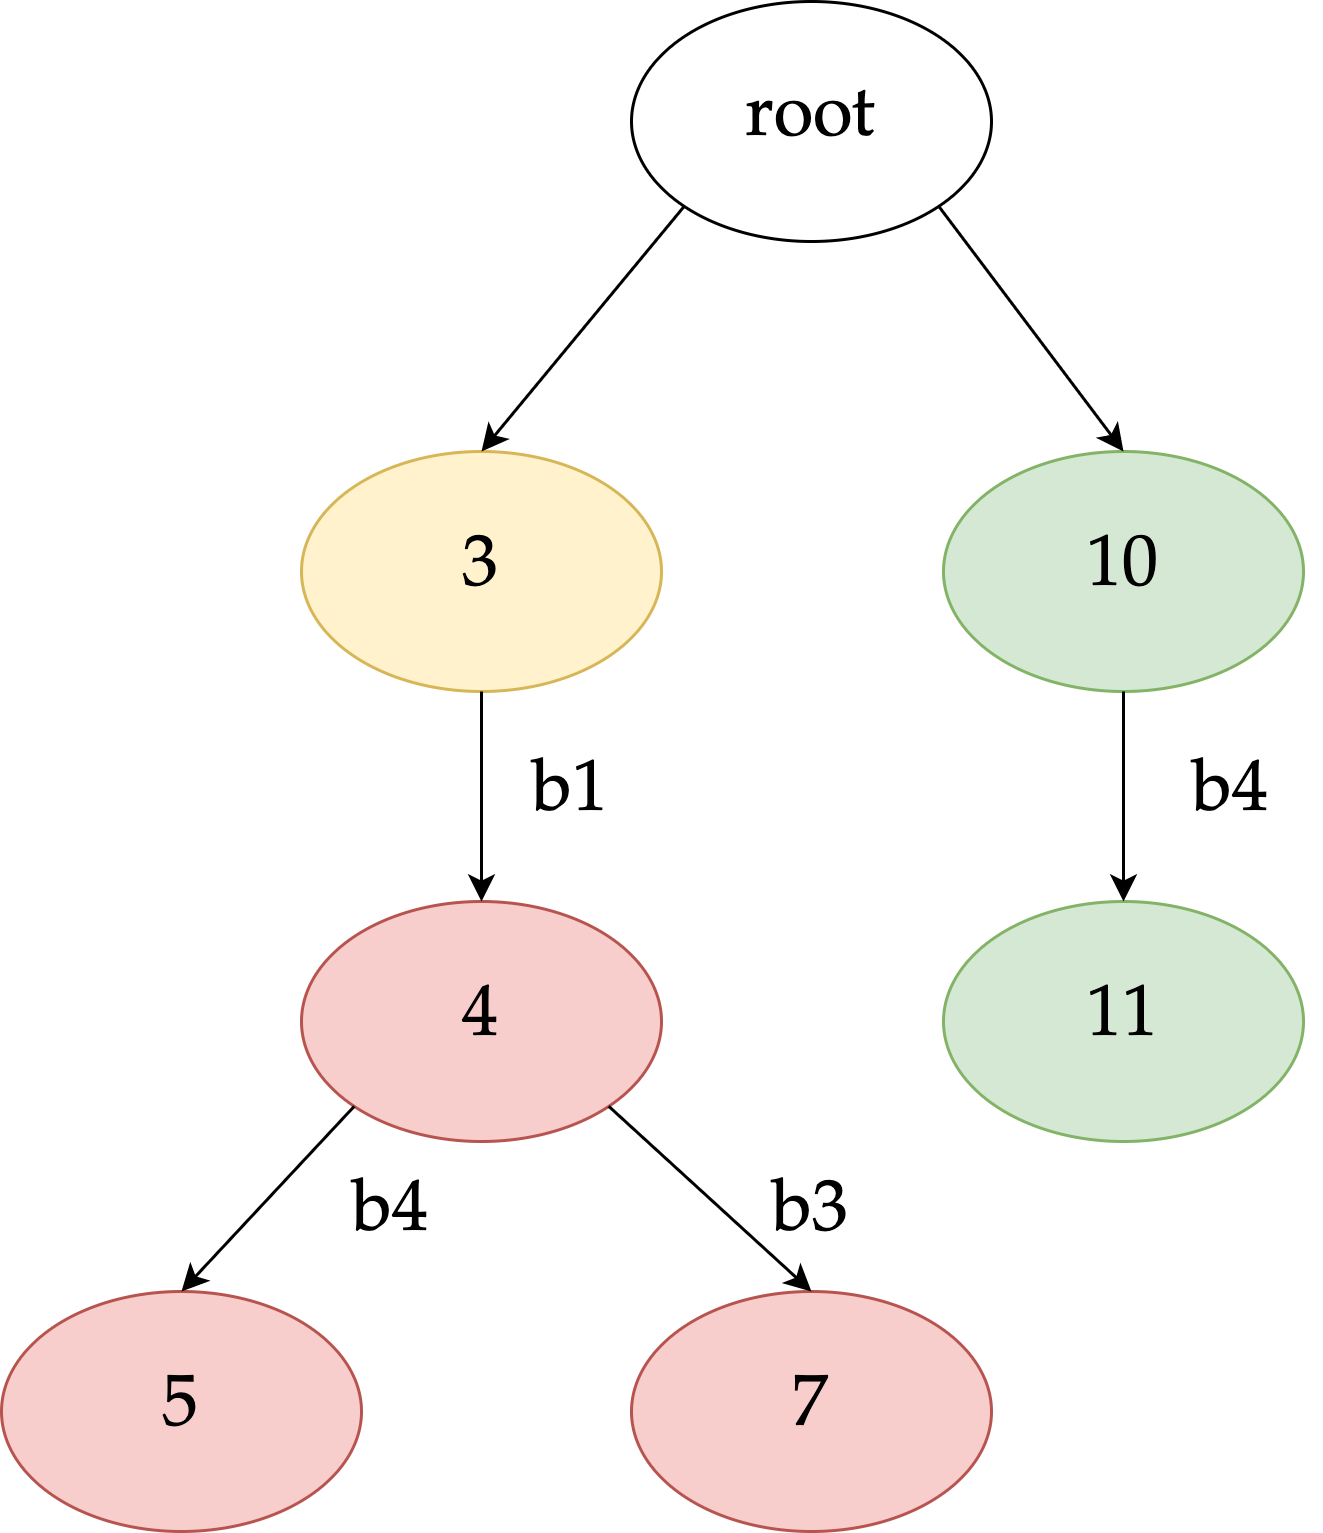
\includegraphics[width=0.5\textwidth]{cdg-code-example}
\label{fig:example-control-dependencies}
\end{figure}

TODO DynaMOSA paper explains the terms dominator, post-dominator, dependence and so on.

Panichella et al.~\cite{Panichella2018} therefore introduced the \ac{DynaMOSA}, which adds to \ac{MOSA} the ability to dynamically focus the search on the subset of previously uncovered targets based on the control dependency hierarchy. In this way, uncovered targets that can be reached by other uncovered targets placed higher in the hierarchy are temporarily removed from the list of objectives. They will be added back later when their parents are covered. This is done for the reason that the temporarily removed targets cannot be covered until their parents are covered in the first place, which is attempted by the search focused only on the parents and shall lead to a more effective consumption of the search budget. \Cref{fig:example-control-dependencies} shows the nodes of the control dependence graph that \ac{DynaMOSA} would consider with a given test \code{foo(1, 3, 3)}. Green marks the nodes that are covered by the test, yellow is the node that need to be covered yet, and red nodes are temporarily ignored because they cannot be reached at that point without nodes $3$ and $11$ being covered first. Since \ac{DynaMOSA} optimizes a subset of the targets also considered by \ac{MOSA}, \ac{DynaMOSA} is guaranteed to be at least as efficient. In their experiments, the authors of both algorithms learned that \ac{DynaMOSA} achieved significantly higher coverage than \ac{WSA}, but also \ac{MOSA}, on a dataset consisting of 346 Java classes.



\begin{algorithm}[t]
\caption{DynaMOSA Algorithm~\cite{Panichella2018}}\label{alg:dynamosa}
\begin{algorithmic}
\Input
  \Desc{$U$}{The set of coverage targets of a program}
  \Desc{$M$}{Population size}
  \EndInput
  \Output
  \Desc{$T$}{An evolved test suite}
  \EndOutput
\State $t \gets 0$
\State $P_t \gets RandomPopulation(M)$
\State $archive \gets UpdateArchive(P_t, \emptyset)$

\While{$\neg (search_budget_consumed)$}
    \State $Q_t \gets GenerateOffspring(P_t)$
    \State $archive \gets UpdateArchive(Q_t, archive)$
    \State $R_t \gets P_t \bigcup Q_t$
    \State $F \gets PreferenceSorting(R_t)$
    \State $P_{t + 1} \gets \emptyset$
    \State $d \gets 0$
    \While{$\left| P_{t + 1} \right| + \left| F_d \right| \leq M$}
        \State $CrowdingDistanceAssignment(F_d)$
        \State $P_{t + 1} \gets P_{t + 1} \bigcup F_d$
        \State $d \gets d + 1$
    \EndWhile
    \State $Sort(F_d)$
    \State $P_{t + 1} \gets P_{t + 1} \bigcup F_d[1 : (M - \left| P_{t + 1} \right|)]$
    \State $t \gets t +  1$
\EndWhile
\State $T \gets archive$
\State \Return $T$
\end{algorithmic}
\end{algorithm}

\begin{algorithm}[t]
\caption{$PreferenceSorting(T, M)$~\cite{Panichella2018}}\label{alg:preference-sorting}
\begin{algorithmic}
\Input
  \Desc{$T$}{A set of candidate test cases}
  \Desc{$M$}{Population size}
  \EndInput
  \Output
  \Desc{$F$}{Non-dominated ranking assignment}
  \EndOutput
\State $F_0 \gets \emptyset$
\For{$u_i \in U$ and $u_i$ is uncovered}
\State $t_{best} \gets \textrm{test case in T with minimum objective score for } u_i$
\State $F_0 \gets F_0 \bigcup \{t_{best}\}$
\EndFor

\State $T \gets T - F_0$
\If{$\left| F_0 \right| > M$}
\State $F_1 \gets T$
\Else
\State $U' \gets \{g \in U : u \textrm{ is uncovered}\}$
\State $E \gets FastNonDominatedSort(T, \{u \in U'\})$
\State $d \gets 0$
\For{All non-dominated fronts in $E$}
\State $F_{d + 1} \gets E_d$
\EndFor
\EndIf

\State \Return $F$
\end{algorithmic}
\end{algorithm}

\begin{algorithm}[t]
\caption{$UpdateArchive(T, A)$~\cite{Panichella2018}}\label{alg:update-archive}
\begin{algorithmic}
\Input
  \Desc{$T$}{A set of candidate test cases}
  \Desc{$A$}{An archive}
  \EndInput
  \Output
  \Desc{$A$}{An updated archive}
  \EndOutput
\For{$u_i \in U$}
\State $t_{best} \gets \emptyset$
\State $best\_length \gets \inf$
\If{$u_i$ already covered}
\State{$t_{best} \gets$ test case in $A$ covering $u_i$}
\State{$best\_length \gets$ number of statements in $t_{best}$}
\EndIf

\For{$t_j \in T$}
\State{$score \gets$ objective score of $t_j$ for target $u_i$}
\State{$length \gets$ number of statements in $t_j$}
\If{$score == 0$ and $length \leq best\_length$}
\State{replace $t_{best}$ with $t_j$ in $A$}
\State $t_{best} \gets t_j$
\State $best\_length \gets length$
\EndIf
\EndFor
\EndFor
\State \Return $F$
\end{algorithmic}
\end{algorithm}

\begin{algorithm}[t]
\caption{$CrowdingDistanceAssignment(T, M)$~\cite{Deb_2000}}\label{alg:crowding-distance-assignment}
\begin{algorithmic}
\Input
  \Desc{$T$}{A set of candidate test cases}
  \Desc{$M$}{A set of objectives}
\EndInput
\State{$l \gets \left|T\right|$}


\For{$i \in T$}
  \State{$T[i]_{distance} \gets 0$}
\EndFor

\For{$m \in M$}
  \State{$T \gets sort(I, m)$}
  \State{$T[1]_{distance} = I[l]_{distance} = \infty$}
  \For{$i = 2$ to $(l - 1)$}
    \State{$T[i]_{distance} \gets T[i]_{distance} + (T[i + 1].m - T[i - 1].m)$}
  \EndFor
\EndFor
\end{algorithmic}
\end{algorithm}

\section{Automatically Generated Oracles}
\label{sec:generated-oracles}
% TODO Teil davon ist Frasers Paper 1600 Bugs in 100 Projects
Traditionally, \ac{SBST} is applied to generate test suites that maximize some coverage criteria, e.g., branch coverage. However, search-based techniques usually do not make any use of automated oracles~\cite{Fraser2013}. A lack of formal specification of the behavior of a program results in generated tests that generally must be supplemented with oracles manually. Davis and Weyuker~\cite{10.1145/800175.809889} introduced the term \textit{non-testable programs}, which includes those programs for which there is no test oracle or a test oracle is impractical to implement, and thus one cannot check the result of the computation for correctness. This includes programs that were either created to know the the outcoming result in the first place, or programs that give too many results to check them all, or the developer had misunderstood the specification. To solve the problem of missing oracles, the authors introduced so-called pseudo oracle. A pseudo-oracle is a second, independently implemented program that must comply with the same specification. It is important for the two versions to be created by separate teams with no intermediary communication so that no misunderstandings can propagate from one team to the other. Afterwards, the results of the computations of the original program and the pseudo oracle can be compared and a decision on validity can be made.

Hiring a second team of developers for this task is definitely too time-consuming and expensive for most software. And so there have been attempts to automate this process. Korel and Al-Yami~\cite{Korel1996} described an approach that uses search techniques to try to find violations to assertions in code. An assertion is simply a conditional whose \texttt{false} branch is assumed to not being executed. However, genetic or symbolic search can be used to explicitly look for a program state that violates the the assertion. An assertion violation leads in most programming languages to some sort of program crash, which in fact is the most basic variant of an automated oracle since an unexpected crash is a bad sign in most cases. 

Romano et al.~\cite{Romano2011} proposed to statically select possible paths that cause memory access violations and look for inputs that direct execution into those paths. It is also possible to represent arithmetic errors such as division by zero as paths, so traditional \ac{SBST} metrics like branch distance can optimize the search towards those errors~\cite{Bhattacharya2011}. Such techniques are called \textit{testability transformations} and were first (\textbf{sicher?}) proposed by Harman et al.~\cite{Harman2004}. Those are often source-to-source transformations intended to improve the performance of various test generation algorithms. McMinn~\cite{McMinn2009} picked up the idea and proposed to automatically generate pseudooracles for a given program. He applied testability transformations to modify the original program and generate a second version that is expected to have the same outputs as the original, but may have discrepancies. To this end, he provided two examples, floating-point arithmetic and multithreading in Java. In the former, for instance, additions between primitive floating-point types, which are somewhat imprecise in the trailing decimal digits according to the IEEE standard~\cite{10.1145/103162.103163}, are swapped by Java's BigDecimal during a transformation, e.g., the calculation $0.1 + 0.1 + 0.1$ in Java yields ~$0.300000000000004$ instead of~$0.3$ (see~\Cref{lst:java-transformations}).

\begin{lstlisting}[language=Java, style=boxed, caption={Comparing floating-point arithmetic in Java using double compared to \code{BigDecimal}~\cite{McMinn2009}}, label=lst:java-transformations]
System.out.println(0.1 + 0.1 + 0.1);
// Output: 0.30000000000000004

System.out.println(
    new BigDecimal("0.1").add(
        new BigDecimal("0.1").add(
            new BigDecimal("0.1")
        )
    )
);
// Output: 0.3
\end{lstlisting}

In his second example, McMinn applies transformations to serialize and deserialize a multithreaded program. Here, methods of a class are provided with Java's \texttt{synchronize} or the keyword is removed if a method is already synchronized. \texttt{synchronize} ensures that only one thread may use the respective method at the same time. In their evaluation, the author tries to use the oracles generated by transforming the respective \ac{SUT} for a genetic-based search for input data which maximize the discrepancy between the outputs of the original program and its pseudooracle. This can not only automatically detect potential bugs (discrepancy), but also measure their severity (size of discrepancy). The idea of automataically generated pseudooracles was also taken up by Fraser and Arkuri~\cite{Fraser_2013} in their search-based test generator \textsc{EvoSuite}.

% TODO reword{}

Transformations have not only been applied in the context of search: the idea to check error conditions was first mentioned in 1976 by Clarke~\cite{Clarke1976} in the context of symbolic execution. Active Property Checking~\cite{Godefroid_2005} describes the use of explicit error branches in the path constraints during \ac{DSE}. By having explicit constraints on the error conditions, \ac{DSE} exploration will try to negate also the error conditions, such that if there exist an input that leads to the error it will be found. This is also implemented in other state-of-the-art \ac{DSE} tools, e.g., Pex~\cite{Tillmann2008} automatically adds constraints that check references against null, divisions against zero, etc. Barr et al.~\cite{Barr2013} instrument programs with additional branches to find floating point exceptions with symbolic execution. These addtional constraints are similar to the error conditions we instroduce in the \ac{MIR} transformation (see \Cref{sec:mir-testability-transformations}), even though some of them are not applicable to Rust due to language pecularities, e.g., there no concept of null pointers.

\clearpage
\chapter{State of the Art}
\label{chap:state-of-the-art}
We give an overview over work that is related to ours in this chapter. 

\section{Fuzzer for Rust}
% TODO reword
Fuzzing is a widely-adopted testing method that exercises a program by automatically generating inputs in a random or heuristic way. However, fuzzing approaches require definition of fuzz targets. A fuzz target defines an array of bytes as input for executing a program composed with some \acp{API}~\cite{Jiang2021}. Fuzzing tools can mutate the input of fuzz targets to explore different paths in \ac{SUT}. \Cref{lst:fuzz-target-example} shows an example of a fuzz target for the example \ac{SUT} \texttt{ex\_lib}.

\begin{lstlisting}[style=boxed, caption={A sample problem for fuzz target generation~\cite{Jiang2021}}, label=lst:fuzz-target-example]
mod ex_lib {
  struct S1;
  struct S2;
  fn f1(a: i16) -> S1;
  fn f2(b: u32) -> S2;
  fn f3(c: &[u8]) -> S2;
  fn f4(s1: S1, s2: &mut S2) -> S2;
  fn f5(s2: &S2, d: &str);
}

fn example_fuzz_target_1(data: &[u8]) {
  if data.len() > 3 {return;}
  let a = to_i16(data, 0);
  let c = to_slice::<u8>(data, 2, data.len());
  let s1 = ex_lib::f1(a);
  let mut s2 = ex_lib::f3(c);
  let _ = ex_lib::f4(s1, &mut s2);
}
\end{lstlisting}

\textbf{AFL++} is a reengineered fork of the popular coverage-guided fuzzer \textsc{AFL} by Zalewski~\cite{Zalewski2014}. It is an extensible community-driven open-source tool that incorporates state-of-the-art fuzzing research. The tool mutates a set of test cases to reach previously unexplored points in the program. The test case triggering new coverage is saved as part of the test case queue~\cite{Fioraldi2020}. Researchers can easily extend the current implementation with additional techniques and use the tool as a baseline for evaluating new ideas. \textit{afl.rs} provides the ability to apply \textsc{AFL++} to Rust.

Another fuzzer can be used in combination with Rust programs is the \textbf{LLVM libFuzzer}, which is coverage-guided evolutionary fuzzing engine. It feeds fuzzed inputs to the library under test via specific fuzzing entry points, also known as \textit{target functions}. The fuzzer tracks which areas of the code are reached and generates mutations on the corpus of input data to maximize the code coverage. Some other tools build upon the libFuzzer and extend it with techniques like concolic testing~\cite{Rocha2020,Le2019}. Both LLVM libFuzzer and \textsc{AFL++} require manually written fuzz targets to be provided, however, i.e., a recipe where to put the generated data into.

\textsc{RULF} is a fuzz target generator which, given the \ac{API} specification of a Rust library, can generate a set of fuzz targets and seamlessly integrate them with \textsc{AFL++} for fuzzing~\cite{Jiang2021}. The approach leverages a sophisticated traversal algoeithm, which can achieve high \ac{API} coverage with only a small set of shallow fuzz targets. To construct fuzz targets, the builds an \ac{API} dependence graph and analyses which \ac{API} calls return values of the type used as a parameter for other \ac{API} calls of the same \ac{SUT}. Using their approach, the autors discovered several bugs in popular Rust libraries. An important limitation of the tool is its inability to analyze generic components and generate fuzz targets for them.

\section{Test Generators for Rust}
% Es gibt eine Reihe von Tools, die für eine automatische Generierung von Tests auf DSE setzen, zum Beispiel \textsc{CUTE}, \textsc{jCUTE}~\cite{Sen2006} und \textsc{KLEE}~\cite{cadar2008klee}. KLEE hat zwei Ziele: (1) das Tool versucht, jede ausführbare Zeile in einem Programm auszuführen, d. h. hohe Statement Coverage zu erreichen und (2) bei jeder gefährlichen Operation (z. B. dereference, assertion) wird versucht zu überprüfen, ob es Werte gibt, die dabei zu einem Fehler führen könnten. Das letztere wird durch symbolische Ausführung erreicht. Da selbst in einfachen Programmen die Anzahl von Ausführungszuständen / -pfaden explodieren kann, wird von \textsc{KLEE} eine Reihe von Heuristiken und Optimisierungstechniken angewendet, um die Performanz zu erhöhen. Zum Beispiel werden nicht ganze Bäume bei Verzweigungen gecloned (Zustände sind nämlich Bäume), sondern es wird der write-on-copy Ansatz auf Objekt-Level angewendet. Unveränderte Teilbäume können von mehreren verschiedenen Zuständen referenziert werden. Außerdem wird versucht, Anfragen an den SAT Solver, um symbolische Werte in konkrete umzuwandeln, so weit vereinfacht wie möglich, da die Verarbeitungszeit der Anfragen, im Allgemeinen NP-vollständig sind~\cite{Lewis1983}, alles andere dominiert. Auf diese Weise konnten die Autoren die Ausführungszeit des Tools auf den GNU Coreutils um das 15-fache beschleunigen.

There are a number of tools that rely on \ac{DSE} for automatic generation of tests, for example \textsc{CUTE}, \textsc{jCUTE}~\cite{Sen2006}, and \textsc{KLEE}~\cite{cadar2008klee}. \textsc{KLEE} has two goals: (1) the tool tries to execute every executable line in a program, i.e., to achieve high statement coverage, and (2) for every dangerous operation (e.g., dereference, assertion), it tries to check whether there are values that could lead to an error in the process. The latter is achieved by symbolic execution. Since even in simple programs the number of execution states/paths can explode, a number of heuristics and optimization techniques are applied by \textsc{KLEE} to increase performance. For example, whole trees are not cloned at branches (states are trees, after all), but the write-on-copy approach is applied at the object level. Unchanged subtrees can be referenced by several different states. Also, requests to the \ac{SMT} solver to convert symbolic values to concrete are attempted to be as simplified as possible, since the processing time of the requests, generally NP-complete are~\cite{Lewis1983}, dominates everything else. In this way, the authors were able to speed up the execution time of the tool on the GNU coreutils by a factor of $15$.

\section{DSE-based Test Generators}
\textbf{\textsc{DART}}~\cite{Godefroid_2005} was the first concolic testing tool that combined dynamic test generation with random testing and model checking techniques to systematically execute all (or as many as possible) feasible paths of a program, while checking each execution for various types of errors.


\textbf{\textsc{CUTE}} (Concolic Unit Testing Engine) and \textbf{\textsc{jCUTE}} (CUTE for Java)~\cite{Sen2006} are also two tools that can generate minimal tests, including input data for C as well as Java programs using \ac{DSE}, respectively. The tools extend \textsc{DART} and generate random input data to initiate search and progress when symbolic execution fails to progress due to their aforementioned limitations. In addition, multithreaded programs are handled that manipulate dynamic data structures using pointer operations. \textsc{CUTE} combines concolic execution with dynamic partial order reduction in multithreaded programs to generate both test inputs and thread schedules systematically. During an evaluation with popular open-source libraries and Java Standard Library, some real bugs were discovered.


\textbf{\textsc{KLEE}} redesigns its predecessor \textsc{EXE}~\cite{Cadar2008} and is built on top of LLVM compiler infrastructure. It uses the \ac{IR} emitted during compilation. The tool performs mixed concrete/symbolic execution, models memory with bit-level accuracy, employs a variety of constraint solving optimization and uses search heuristics to get high code coverage. In addition, for each dangerous operation (e.g., dereference, assertion), the tool tries to check whether there are values that could lead to an error in the process. In the experiments, the tool generated tests that exceeded the coverage of manually written tests by far and could find bugs even in such commonly used tools as parts of the GNU Coreutils. Since even in simple programs, the number of execution states/paths can explode, \textsc{KLEE} applies multiple heuristics and optimization techniques to improve performance. For instance, whole trees are not cloned at decision branches (states are, after all, trees). Instead, the write-on-copy approach is applied at the object level. Several different states can reference unchanged subtrees. Moreover, requests to the \ac{SMT} solver to convert symbolic values into concrete ones are attempted to be as simplified as possible since the requests' processing time dominates everything else. In this way, the authors were able to speed up the execution time of the tool on the GNU Coreutils by 15 times. With the birth of Rust, it was later possible to apply KLEE to the LLVM IR of the Rust compiler.

The authors of \textsc{KLOVER}~\cite{Li2011} describe the tool as the first to allow symbolic execution and test generation for industrial C++ programs. It builds on top of \textsc{KLEE}, works with the LLVM bitcode, and extends \textsc{KLEE}'s optimizations to C++ language features, for example, classes and objects and LLVM intrinsics.


\section{Search-based Test Generators}
\textbf{\textsc{EvoSuite}}~\cite{Fraser_2011} is a tool that automates the task of generating unit tests by systematically producing test suites that achieve high coverage, are as small as possible, and provide assertions. \textsc{EvoSuite} uses not only a search-based approach but also exploits \ac{DSE}, hybrid search, and testability transformations~\cite{Harman2004} to improve its efficiency. The tool targets programs that do not have any formal specification, which could be used to derive oracles to test the actual behavior against the expected one. However, it uses mutation testing to produce a reduced set of assertions. These assertions highlight the relevant aspects of the current behavior in order to support developers in identifying defects. Originally, \textsc{EvoSuite} used to apply the \ac{WS} approach but has switched to \ac{DynaMOSA} ever since. The tool sets the bar for the quality of automatically generated tests~\cite{Vogl2021,Panichella2020,Campos2019,Fraser2018,Fraser2016,Fraser2017}.

\textbf{SUSHI}~\cite{Braione2018} is an open-source test generator for Java that combines both concolic and evolutionary testing. It does the latter by leveraging \textsc{EvoSuite}. The tool tries to synthesize test suites with high branch coverage. It explores the program execution space and computes the execution conditions of the program paths. Afterward, the path conditions will be translated into executable evaluators that quantify the distance of a concrete state from satisfying the corresponding path condition.

\textbf{EvoObj}~\cite{Lin2021} is an extension to \textsc{EvoSuite}. The tool tackles the problem that the effectiveness of \ac{SBST} suffers greatly when generating complex object inputs due to search spaces that are neither continuous nor monotonic. The tool employs analysis of static control and data flow of a \ac{SUT} to create \textit{seed tests}. The seed tests can drastically increase the performance of the search by providing a more continuous and monotonic fitness landscape.

\section{Random Testing Tools}
\textbf{Randoop}~\cite{Pacheco_2007} generates unit tests for Java code using feedback-directed random test generation. Feedback-directed random testing uses execution feedback gathered from executing test inputs as they are created to avoid generating redundant and illegal inputs. Randoop can verify some basic assumptions on programs. For instance, in general, programs should not crash, which is a sort of automated oracle. The tool can also check  contracts on the code, which may be supplied by the user. By default, it implements multiple default contracts that are employed in the Java language, e.g., reflexivity of \textit{Object.equals}~\cite{Fraser2013}. Randoop outputs two test suites; one contains contract-violating tests, and the other contains \textit{regression} tests, which do not violate contracts but instead capture an aspect of the current implementation of a \ac{SUT}. Those can discover inconsistencies between two versions of a software.


\clearpage
\chapter{Rust Programing Language}
\label{chap:rust-programming-language}
% TODO das sollte natürlich umformuliert werden
The Rust programming language is an increasingly popular language, designed to be fast, efficient, and safe. Design on the language began in 2006, with the first stable version being released in 2015. The high level goals of the language are to provide performance comparable to systems programming languages like C and C++, but without sacrificing the safety of higher-level languages, like Java and Python.

This is a difficult problem to solve, because the systems programming languages need to be able to control how memory is managed explicitly in order to be performant, which is easy to do incorrectly. The higher-level languages sacrifice this control for convenience, using tools such as garbage collectors to automate memory management.
Consider, as an example, how heap memory is handled in C and Java. In C we can allocate memory on the heap by using the \texttt{malloc} or \texttt{calloc} functions. The data on the heap can then be reclaimed with \texttt{free}. These functions are easily misused, e.g., by calling free twice on the same pointer, which leads to undefined behaviour, and forgetting to free memory would be wasting that memory. Java, and many other high level programming languages, use a different approach. Here the programmer does not have to manually allocate and deallocate heap memory, but it is reclaimed at runtime using a garbage collector. While this makes it easier to write programs that correctly handle memory, it also impacts program performance, due to the operational overhead of determining which memory is no longer in use.

In Rust, this problem is addressed by the ownership system, which requires that the code is written in such a way that the compiler can infer when memory should be allocated, and released to the allocator. If the code does not satisfy the requirements, it will not compile.

\section{Tooling}
Rust comes with official package managers, which we briefly describe in the following sections.

\subsection{Cargo}
Cargo is the name of Rust’s package manager, which is provided out-of-the-box. It can be used to create new packages, download dependencies and compile packages. More advanced features supported by Cargo are publishing packages and running tests. Packages created and used by cargo are known as crates. Cargo is designed to be the central tool which developers use when working with crates. When programs have the cargo prefix, Cargo will forward function calls to them as if they were called without the prefix, providing information on the crate in the context that it was called. Tools like Clippy work in this way.

\subsection{Rustup}
While Cargo is used to manage crates, Rustup is used to manage Rust tools, like Cargo and the Rust compiler, and any other components which have been added to the toolchain. Among other things, Rustup makes it possible to have fine-grained control over the version of Rust used to compile crates. To understand how this affects development, we explain the versioning used in the Rust ecosystem. New stable and beta versions of Rust are released every six weeks, and a nightly version is released every night, based on the previous day's master branch in the central git repository. The beta versions are based on the latest nightly every six weeks, and the stable versions are based on the previous beta.
Features introduced in nightly versions of the compiler must be explicitly enabled in the source code, as shown in \Cref{lst:example-enable-feature}.

\begin{lstlisting}[style=boxed, caption=Enabling features in Rust, label=lst:example-enable-feature]
#![features(box_patterns)]
\end{lstlisting}

In order to develop any sort of tooling for Rust, developers must use nightly versions, although they can pin the version to a certain date if they wish.
Rustup allows developers to set the version specifically for a given project, or as a global default.

\section{Language Basics}
The Rust language itself is unique in many ways, and we strive to summarize the key points in the following subsections.

\subsection{Syntax}
Rust syntax is mostly in line with the C family of languages. The ubiquitous Hello, World! program can be written as shown in \Cref{lst:example-hello-world}.
\begin{lstlisting}[style=boxed, caption=Hello World, label=lst:example-hello-world]
println!("Hello World!");
\end{lstlisting}

In \Cref{lst:example-struct-enum} we demonstrate a struct and an enum type definition with generics. The generics are indicated by the angle brackets, and in this case are two anonymous type parameters. Enums and structs are the two central types available in Rust. Enums are accessed via pattern matching, whereas struct fields can be accessed directly. While curly brackes indicate scope, and statements end with a semicolon, Rust differs from the C family of languages in that its function definitions do not start with the return type. Typically, in fact, the types are written after the identifiers, as demonstrated in \Cref{lst:example-functions-struct-enum}.

\begin{lstlisting}[style=boxed, caption={The type definition for a point in two-dimensional space and an enum definition}, label=lst:example-struct-enum]
struct Point {
  x: f64,
  y: f64
}

enum Result<T, E> {
  Ok(T),
  Err(E)
}
\end{lstlisting}


\begin{lstlisting}[style=boxed, caption={A function to compute the point between two points in two-dimensional space}, label=lst:example-functions-struct-enum]
fn middle(p1: Point, p2: Point) -> Point {
  Point {
    x: (p1.x + p2.x) / 2,
    y: (p1.y + p2.y) / 2
  }
}
\end{lstlisting}

In \Cref{lst:example-functions-struct-enum}, we compute and return a new point, placed in between the two points provided. This may look strange to those used to seeing the return keyword used instead. While it is possible to return values in that way, it is considered idiomatic Rust to return by ending the function with an expression, which is implicitly interpreted by the compiler as a return statement.

\subsection{Associated Functions and Methods}
Functions can be associated with types in Rust, e.g., with enums or structs. Rust separates the definition of behavior from the definition of data. To implement behavior for an enum or a struct, we add an \texttt{impl} block, as shown in \Cref{lst:example-associated-function}. An example of a common associated function is a \texttt{new} function that returns a value of the type the associated function is associated with.

\begin{lstlisting}[style=boxed, caption={Associating behavior with the \texttt{Point} data type defined in \Cref{lst:example-struct-enum}}, label=lst:example-associated-function]
impl Point {
  fn new(x: f64, y: f64) -> Self {
    Self { x, y }
  }
}

let p = Point::new(32.0f32, 42.0f32);
\end{lstlisting}

Associated functions whose first parameter is named \texttt{self} are called methods and may be invoked using the method call parameter, for instance, \texttt{x.foo()}, as well as the usual function call annotation. That is, \texttt{self} is an instance of the type and an owner of the method. Through \texttt{self}, we can access the state and methods of the instance, e.g., as in \Cref{lst:example-method}.

\begin{lstlisting}[style=boxed, caption={Defining a method on \texttt{Point} data type from \Cref{lst:example-struct-enum}}, label=lst:example-method]
impl Point {
  fn new(x: f64, y: f64) -> Self {
    Self { x, y }
  }

  fn add(&self, other: &Self) -> Self {
    Self {
      x: self.x + other.x,
      y: self.y + other.y
    }
  }
}

let p1 = Point::new(32.0f64, 42.0f64);
let p2 = Point::new(10.0f64, 10.0f64);

let result = p1.add(&p2);

// Same as

let result2 = Point::add(&p1, &p2);
\end{lstlisting}


\subsection{Traits}
A trait describes an abstract interface that types can implement. This interface consists of associated items, which come in three varieties: functions, types, constants. All traits define an implicit type parameter \texttt{Self} that refers to ''the type that is implementing this interface''. Traits are implemented for specific types through separate implementation blocks. If the trait function defines a body, this definition acts as a default for any implementation which does not override it. Otherwise, the trait indicates that the implementor must define the function. Similarly, associated constants may omit the equals sign and expression to indicate implementations must define the constant value. Associated types must never define the type, the type may only be specified in an implementation. As an example, a trait could be defined for implementing a method that generates a string from an instance of a type, as shown in \Cref{lst:example-trait}.

\begin{lstlisting}[style=boxed, caption={Trait definition and implementation for the \texttt{Point} data type from \Cref{lst:example-struct-enum}}, label=lst:example-trait]
trait ToString {
  fn to_string(&self) -> String;
}

impl ToString for Point {
  fn to_string(&self) -> String {
    format!("({}, {})", self.x, self.y)
  }
}

let p = Point::new(32.0f64, 42.0f64);
let textual_repr = p.to_string();
\end{lstlisting}

% When the associated function is declared on a trait, the function can also be called with a path that is a path to the trait appended by the name of the trait. When this happens, it is substituted for \texttt{<_ as Trait>::function_name}.

\subsection{Generics and Trait Objects}
% TODO reword
Rust supports generic types and allows for shared behavior via traits. Generics parametrize data structures, methods, and functions, such that the same code can be used with different types. This improves usability and helps finding type errors statically. The language provides static and dynamic dispatch. The former is realized by means of monomorphization, i.e., for each type a generic function is used with, the compiler generates a concrete implementation of it for the respective type and replaces the call sites with calls to these specialized functions. As a consequence, the final binary will be slightly larger due to potentially many copies of the same code, but calling the functions will not result in any runtime overhead. Moreover, due to static type information, the compiler can inline the code, which in general leads to a better performance. \Cref{lst:static-dispatch} demonstrates a generic data type which uses static dispatch.

\begin{lstlisting}[style=boxed, caption={A data type with static dispatch via monomorphization}, label=lst:static-dispatch]
struct Pair<L, R> {
  left: L,
  right: R
}

impl<L, R> Pair<L, R> {
  pub fn of(left: L, right: R) -> Self {
    Pair { left, right }
  }

  pub fn left(&self) -> &L {
    &self.left
  }

  pub fn right(&self) -> &R {
    &self.right
  }
}
\end{lstlisting}

% TODO reword
With dynamic dispatch, trait objects come into play. Trait objects are normal values that store a value of any type that implements the given trait, where the precise type can only be known at runtime. The methods of the trait can be called on a trait object via the \textit{vtable}, which is created an managed by the compiler. A function that takes trait objects is not specialized to each type that implements the trait: only one copy of the code is generated, which usually results in less code bloat. However, this comes at the cost of requiring slower virtual function calls, and effectively inhibiting any chance of inlining and related optimizations from occuring. When using trait objects, they must be packed into a data type with known size at compile time, e.g., a \texttt{Box}, which is a pointer into the heap, as demonstrated in \Cref{lst:dynamic-dispatch}.

\begin{lstlisting}[style=boxed, caption=A data type with dynamic dispatch, label=lst:dynamic-dispatch]
struct Pair {
  left: Box<dyn Any>,
  right: Box<dyn Any>
}


impl Pair {
  pub fn of(left: Box<dyn Any>, right: Box<dyn Any>)
    -> Self {
    Pair { left, right }
  }

  pub fn left(&self) -> &Box<dyn Any> {
    &self.left
  }

  pub fn right(&self) -> &Box<dyn Any> {
    &self.right
  }
}
\end{lstlisting}

With the definition from \Cref{lst:static-dispatch}, we can now create \texttt{Pair} instances with different types as shown in \Cref{lst:example-generics-usage} using monomorphization, e.g., \texttt{String} and \texttt{u32} or two times \texttt{usize}. The same code is reused and the compiler can statically check whether the values that are used with a pair instance are of the correct type:
\begin{lstlisting}[style=boxed, caption={}, label=lst:example-generics-usage]
fn main() {
  let pair: Pair<String, u32> = Pair::of(
    "Hello world".to_string(), 42u32
  );
  let left_value: &str = pair.left();

  let another_pair: Pair<usize, usize> = Pair::of(
    0usize, 1usize
  );
}
\end{lstlisting}
The compiler can now extract the relevant types and generate the following code

It is also possible to put constraits, which are called trait bounds in Rust, on the type parameters. For instance, we could define a textual representation of a pair. The \texttt{Display} trait of the standard library defines the \texttt{fmt} method which uses the \texttt{\string{\string}} print marker. As shown in \Cref{lst:example-trait-bounds}, in order for a type to implement a trait, it's attributes must have implemented the trait, too. Hence, we tell that the left and right hand side type parameters used with the \texttt{Pair} struct must implement the \texttt{Display} trait. The effect of bounding is that generic instances are allowed to access the methods of traits specified in the bounds. Under the hood, the \texttt{println!} macro call the \texttt{fmt} method of the \texttt{Pair} instance:
\begin{lstlisting}[style=boxed, caption={}, label=lst:example-trait-bounds]
struct Pair<L: Display, R: Display> {
    left: L,
    right: R
}

impl<L: Display, R: Display> Pair<L, R> {
  pub fn of(left: L, right: R) -> Self {
    Pair { left, right }
  }
}

impl<L: Display, R: Display> Display for Pair<L, R> {
  fn fmt(&self, f: &mut std::fmt::Formatter)
      -> std::fmt::Result {
    write!(f, "({}, {})", self.left, self.right)
  }
}

fn main() {
  let pair: Pair<String, u32> = Pair::of(
    "Hello world".to_string(), 42u32
  );
  println!("{}", pair);
  // Output: (Hello world, 42)
}
\end{lstlisting}

There is no inheritance in Rust, as known from object-oriented languages. Common behavior can be defined via traits, which can have supertraits, as shown in \Cref{lst:trying-supertraits} for the \texttt{TrieAtom} trait. Implementors of the trait must also implement the other four traits:
\begin{lstlisting}[style=boxed, caption={An example trait from the \textit{trying} crate which we evaluate the approach on}, label=lst:trying-supertraits]
pub trait TrieAtom: Copy + Default + PartialEq + Ord {}
\end{lstlisting}

Besides structs, it is also possible to parametrize methods and functions using generics. A generic method or function has a type parameter which is inferred from the values passed as parameters. An example for
\begin{lstlisting}[style=boxed, caption={Variants of defining a generic function}, label=lst:function-monomorphization]
fn make_pair<L: Display, R: Display>(left: L, right: R)
    -> Pair<L, R> {
  Pair::of(left, right)
}

// Alternative syntax for monomorphism,
// useful when the definition grows large
fn make_pair<L, R>(left: L, right: R) -> Pair<L, R>
where L: Display, R: Display {
  Pair::of(left, right)
}

fn main() {
  let pair: Pair<String, String> = make_pair(
    "Hello".to_string(),
    "world".to_string()
  );
  let another_pair: Pair<usize, u32> = make_pair(
    4usize, 2u32
  );
}
\end{lstlisting}

The function \texttt{make\string_pair} creates a generic \texttt{Pair} instance. Then, the same generic function is used to create a pair of two strings and a pair of a \texttt{usize} and a \texttt{u32}.

Traits may also contain additional type parameters. These type parameters may be constrained by other trait and so forth, see \Cref{lst:traits-with-type-bounds}. Usually, the more constraints, the more difficult it is to find correct types and automatically generate test cases that use those features and do compile.

\begin{lstlisting}[style=boxed, caption={Type parameters can be specified for a trait to make it generic. These appear after the trait name, using the same syntax used in generic functions}, label=lst:traits-with-type-bounds]
trait PrintableSeq<T: Display> {
  fn len(&self) -> usize;
  fn at(&self, pos: usize) -> T;
  fn iter<F>(&self, f: F) -> where F: Fn(T);
}
\end{lstlisting}

\subsection{Ownership and Borrowing}
As mentioned in the beginning of the chapter, Rust has an approach to memory management which is different from the classical approach of C or C++, where memory is managed manually through functions like \texttt{malloc} and \texttt{free}, or by letting the garbage collector manage the resources. In Rust, each value has a variable that's called its owner. There can only be one owner of a value at a time, and once the owner goes out of scope, the value is deallocated.

\begin{lstlisting}[style=boxed, caption=Heap data owned by binding, label=lst:example-ownership]
{
  // The String data on the heap is created
  // and set to be owned by binding a
  let a = String::from("content");
}
// The scope in which a is active is over,
// and a is now no longer valid. At the same
// time the string data on the heap is freed
\end{lstlisting}

In cases where the value needs to outlive a given scope, it can be moved to a new owner in a different scope. This happens, for example, when a value is passed as a parameter to a function, or on assignment, with the caveat that some values are so cheaply copied that a move is never necessary.

\begin{lstlisting}[style=boxed, caption=Transferring Ownership, label=lst:transfer-ownership]
let b;
{
    let a = String::from("content");
    b = a;

    println!("The content is: {}", a);
    // Trying to use a after transferring the
    // ownership results in a compilation error
}
\end{lstlisting}

This would quickly become burdensome in cases where a value needs to be passed to a function, and then used again later. For that case, we have references, which can be immutable, or read-only, or mutable, meaning that the owner of the reference has direct access to the underlying value as well. When a reference is taken, it is known as borrowing in Rust, and is a key interaction in the ownership model. When a value is borrowed, the owner is unable to modify it. A value can only be borrowed mutably if no other borrow is valid for the duration of the borrow. A value can be borrowed immutably multiple times, as there is no possibility of a race condition when the underlying cannot be modified. These rules make it possible to infer when resources can be deallocated, and guarantee memory safety, but also make it impossible to create structures that are not tree-formed. For example, it would be impossible to create a linked list with these conditions. That is because the ownership system is an over-approximation of memory safety, and there are cases where completely valid and safe code can be written, which does not satisfy its conditions. This is why much of the standard library is implemented using the \texttt{unsafe} keyword, which allows the programmer, among other things, to bypass these rules. In practice, this means that memory bugs still happen in Rust, but that the ownership system prevents them from originating in safe Rust.

Ownership spielt auch für die generierten Tests eine wichtige Rolle und macht die Generierung schwieriger, als zum Beispiel in Sprachen wie Java. Das ist zum Beispiel aus \Cref{lst:ownership-method-call} ersichtlich.
\begin{lstlisting}[style=boxed, caption={Transferring the ownership to a method}, label=lst:ownership-method-call]
fn main() {
    let mut message = String::from("Hello");
    print(message); // Value moved here
    // Compile error, value borrowed here after move
    message.push_str(" world!");
}

fn print(message: String) {
  // message gets dropped when the execution
  // goes out of scope
  println!("{}", message);
}
\end{lstlisting}

% Das Problem mit dem oben beschriebenen Ownership-Modell ist, dass wenn man mit dem moved value nach einem Funktionsaufruf weiter arbeiten möchte, wie zum Beispiel in \Cref{lst:ownership-method-call}, muss die aufgerufene Funktion den Wert an die aufrufende Funktion zurückgeben, da im Beispiel der String in die Funktion \texttt{print} bewegt. Stattdessen kann man der aufgerufenen Funktion eine Referenz zum Wert als Argument übergeben, die wie ein Pointer zum Wert ist, sodass die Funktion der Adresse folgen und auf den Wert zugreifen kann. Anders als ein Pointer in C zeigt eine Referenz in Rust garantiert auf den korrekten Speicher. Wie in \Cref{lst:borrowing-method-call} gezeigt, kann eine Referenz auf einen Wert mittels \texttt{&} übergeben werden. Die Syntax \texttt{&message} erlaubt es, eine Referenz zu erstellen, die den Stringwert referenziert, jedoch nicht ownt, das heißt, sie leiht den Wert aus. Da die Referenz den Wert nicht ownt, wird er auch nicht dropped wenn die Referenz nicht mehr verwendet wird.

The problem with the ownership model described above is that if you want to continue working with the moved value after a function call, such as in \Cref{lst:ownership-method-call}, the called function must return the value to the calling function, since in the example the string moved into the function \texttt{print}. Instead, you can pass a reference to the value as an argument to the called function, which is like a pointer to the value, so the function can follow the address and access the value. Unlike a pointer in C, a reference in Rust is guaranteed to point to the correct memory. As shown in \Cref{lst:borrowing-method-call}, a reference to a value can be passed using \texttt{\string&}. The syntax \texttt{\string&message} allows to create a reference that references the string value but does not ownt, that is, it borrows the value. Since the reference does not own the value, the will not be dropped when the reference is no longer used.

\begin{lstlisting}[style=boxed, caption={Transferring the ownership to a method}, label=lst:borrowing-method-call]
fn main() {
    let mut message = String::from("Hello");
    // A reference to message
    // it passed to the function call
    print(&message);
    // Variable message still owns the value
    // after the call
    message.push_str(" world!");
}

// The function borrows the value of message
fn print(message: &String) {
  println!("{}", message);
}
\end{lstlisting}

Whether owner or borrowed, values cannot be changed by default, this is prevented by the compiler. If this is still necessary, it must be explicitly specified with the keyword \texttt{mut}, as in \Cref{lst:mut-borrowing-method-call}.

\begin{lstlisting}[style=boxed, caption=Transferring the ownership to a method, label=lst:mut-borrowing-method-call]
fn main() {
    let mut text = String::from("Hello");
    extend_msg(&mut text);
    println!("{}", &text);
    // Output: Hello world!
}

fn extend_text(text: &mut String) {
    text.push_str(" world!");
}
\end{lstlisting}

Thus, the restrictive ownership model for genetic search has certain implications for the generated tests, namely that variables cannot be used arbitrarily and the ownership or borrows of variables must be observed after certain function and method calls.

\subsection{Lifetimes}
The lifetime of a reference determines the duration it is valid for. Each reference in Rust has a lifetime, and the compiler infers constraints for these lifetimes based on how they are used. The compiler will emit an error if the lifetime constraints cannot be satisfied. Sometimes the compiler requires hints for the relationship between the input and output lifetimes of a function. It will always require annotations on type definitions. This is important for two reasons. First, it allows the compiler to ensure that a reference never outlives the underlying value, and second, it allows the compiler to ensure that there never is an overlap of mutable access to a value.

\section{Overview of the Compiler}
As with most compilers, the Rust compiler (\texttt{rustc}) goes through several phases, each of which uses some \ac{IR} to facilitate computatations. In general, working directly with the source code is extremely inconvinient and error-prone. Source code is designed to be human-friendly while at the same time being unambiguous, but it's less convenient for doing something like type checking.

Instead most compilers, including \texttt{rustc}, build some sort of \ac{IR} out of the source code which is easier to analyze. \texttt{rustc} has a few \acp{IR}, each optimized for different purposes:

\begin{itemize}
    \item Token stream: the lexer produces a stream of tokens directly from the source code. This stream of token is easier for the parser to deal with than raw text.
    \item \ac{AST}: the abstract syntax tree is built from the stream of tokens. It represents almost exactly what a user wrote. It helps to do some syntactic sanity checking (e.g., checking that a type is expected where the user wrote one).
    \item \ac{HIR}: This is a desugared and compiler-friendly representation of the \ac{AST} that is generated after parsing, macro expansion, and name resolution. It's still close to what the user wrote syntactically, but it includes implicit information such as elided lifetimes. Also, some expression forms have been converted to simpler ones, e.g., \texttt{for} loops are converted to a more basic \texttt{loop}. This \ac{IR} is amenable to type checking.
    % Lowering to HIR: https://rustc-dev-guide.rust-lang.org/lowering.html
    \item \ac{THIR}: This is an intermediate between \ac{HIR} and \ac{MIR}. It's similar to \ac{HIR} but it is fully typed and a bit more desugared.
    \item \ac{MIR}: This \ac{IR} is a \ac{CFG}. It shows the basic blocks of a program and how control flow can go between them. A basic block contains simple typed statements (e.g., assignments, simple computations, etc.) and control flow edges to other basic blocks. This representation is used to for borrow checking and other important dataflow-based checks, such as checking uninitialized values.
    \item LLVM \ac{IR}: This is a standard form of all input to the LLVM compiler. LLVM \ac{IR} is a typed assembly language with lots of annotations. It is designed to be easy for other compilers to emit and also rich enough for LLVM to run optimizations on it.
\end{itemize}

\subsection{High-Level Intermediate Representation}
Many parts of the \ac{HIR} resemble Rust surface syntax quite closely, with the exception that some of Rust's expression forms have been desugared away. Für die Analyse von verfügbaren Strukturen, Methoden und Funktionen müssen wir möglichst viele Informationen bekommen, die vom Compiler zur Verfügung gestellt werden. Die \ac{HIR} ist dafür perfekt geeignet, denn auf dieser Ebene werden zugleich die Typen explizit vom Compiler ausgefüllt und es werden noch alle für uns relevante Sprachelemente beibehalten. Lediglich werden intraprozedurale Elemente desugared, for instance, \texttt{for} loops are converted into a \texttt{loop} and do not appear in the \ac{HIR}.
\begin{lstlisting}[style=boxed, caption={An example Rust program that we convert to HIR}, label=lst:hir-lowering]
struct IntVec {
    vec: Vec<i32>
}

impl IntVec {
    pub fn foo(&mut self) {
        for n in self.vec {
            // Does something
        }
    }
}
\end{lstlisting}

\Cref{lst:hir-lowering,lst:hir-lowered} demonstrate a comparison of the same program before and after lowering to \ac{HIR}. The main differences are the desugared \texttt{for} loop and the filled in type declaration of the \texttt{self} parameter of the \texttt{foo} method. Da wir für das Generieren eines Tests für die gegebene \texttt{foo} Methode nur die Methodensignatur sowie die Structdefinition brauchen, stellt das Desugaring kein Problem dar.

\begin{lstlisting}[style=boxed, caption={HIR of the code in \Cref{lst:hir-lowering}}, label=lst:hir-lowered]
struct IntVec {
    vec: Vec<i32>,
}

impl IntVec {
  pub fn foo(self: &mut Self) -> () {
    {
      let _t = match #[lang = "into_iter"](self.vec) {
        mut iter => loop {
          match #[lang = "next"](&mut iter) {
            #[lang = "None"] {} => break,
            #[lang = "Some"] { 0: n } => {
              {
                // Does something
              };
            }
          }
        },
      };
      _t
    }
  }
}
\end{lstlisting}

Bei der nächsten Lowering Stufe, nämlich \ac{THIR}, kennt, ähnlich wie \ac{MIR}, nur function bodies, d. h. nur ausführbaren Code. Folglich hat \ac{THIR} keine Repräsentation für Items wie \texttt{struct} oder
\texttt{trait} und ist daher für diese Art der Analyse nicht hilfreich.

\subsection{Mid-Level Intermediate Representation}
% TODO umformulieren und so
\ac{MIR} is based on the \ac{CFG} of a program and is fully typed. The \ac{MIR} for a given function consists of a series of basic blocks. A basic block is an atomic unit of the program's \ac{CFG}, is guaranteed to execute completely, and is made up of a sequence of statements followed, optionally, by a terminator, which corresponds to an edge in the \ac{CFG}. \ac{MIR}, being very much internal to the Rust compiler, does not have a stable definition and undergoes frequent changes. There is no stable surface syntax for \ac{MIR}, only one intended for debugging, which we will use here to show examples of analysis and instrumentation. Rather it is defined as a collection of data structures. \ac{MIR} has enough information to make our program instrumentation feasible, though its unstable nature makes the consumption of \ac{MIR} challenging to maintain across different toolchain versions.

At this level, each executable piece of code, e.g., a function or a method, is represented as a \texttt{Body} object, which contains information about locals (parameters, user-defined variables, compiler-defined variables, and the return value) and basic blocks.

Locals are memory allocations allocated on the stack (conceptually, at least), such as function arguments, local variables, and temporaries. These are identified by an index, written with a leading underscore, like \texttt{\string_1}. There is also a special local (\texttt{\string_0}) allocated to store the return value. 

Basic blocks consist of statements, which are in terms of \ac{MIR} actions with one successor. The statements of a basic block are mostly definitions of locals, e.g., atomic computations, which are later used by the corresponding terminator. A terminator is an action with potentially mutliple successors and is always placed at the end of a basic block. A terminator can be, for instance, a \texttt{Call} (function call), a \texttt{Return} (returns the \texttt{\string_0} local), a \texttt{Goto} jump (jump to the given block number), a \texttt{SwitchInt}, or an \texttt{Assert}. \textsc{RustyUnit} makes use mainly of \texttt{SwitchInt} and \texttt{Assert} terminators. 

\texttt{SwitchInt} results from lowering \texttt{if} and \texttt{loop} conditions and \texttt{match} expressions. The value of it's operand always evaluates to an integer; the execution jumps depending on its value to one of the targets. There is also a dedicated \texttt{otherwise} value for all other cases. Each possible value (e.g., $0$ and $1$ for \textit{false} and \textit{true}, respectively, in \texttt{if} conditions) has a corresponding basic block which the execution jumps to. Assume that there are two functions, \texttt{cheeky\string_itoa(x: i32)} and \texttt{bold\string_itoa(x: i32)} which both return a string (more precisely, a reference to a static string value) based on the input number, as shown in \Cref{lst:mir-lowering}.

\begin{lstlisting}[style=boxed, caption={HIR of the code in \Cref{lst:hir-lowering}}, label=lst:mir-lowering]
fn cheeky_itoa(x: i32) -> &'static str {
  match x {
    0 => "There is nothing here, 
      only the infinite emptiness",
    42 => "The answer to everything",
    _ => "Must be some huge value"
  }
}

fn bold_itoa(x: i32) -> &'static str {
  if x > 42 {
    "Must be some huge number"
  } else {
    "Not that huge, I'd say"
  }
}
\end{lstlisting}

As mentioned earlier, conditions like those in loops, \texttt{match} and \texttt{if} expressions are converted to \texttt{switchInt} terminators. In \Cref{lst:mir-lowered-first}, the \ac{MIR} for the function \texttt{cheeky\string_itoa} is shown in its debug form. It has been cleaned up for simplicity and usually still includes many debugging comments on the individual statements and terminators. Only two locals are given, the return value \texttt{\string_0} of type \texttt{\string&str} 
and the function parameter \texttt{\string_1} of type \texttt{i32}.

We can see that the entry block, which is always \texttt{bb0}, consists only of the \texttt{switchInt} termiantor, which, based on the value of the function parameter \texttt{\string_1}, directs execution to either block number $2$ (if \texttt{\string_1} is $0$) or $3$ (if \texttt{\string_1} is $42$). If neither case matches, the execution jumps to block $1$. For the decision, the values, which are always integers, are directly compared. Each of the following three blocks defines the return local and points to the last block (\texttt{\string_4}), which returns \texttt{\string_0} to the caller. 

\begin{lstlisting}[style=boxed, caption={\ac{MIR} of the \texttt{cheeky\string_itoa} function}, label=lst:mir-lowered-first]
fn cheeky_itoa(_1: i32) -> &str {
  let mut _0: &str;

  bb0: {
    switchInt(_1) -> [
      0_i32: bb2, 
      42_i32: bb3, 
      otherwise: bb1
    ]; 
  }

  bb1: {
    _0 = const "Must be some huge value"; 
    goto -> bb4;                  
  }

  bb2: {
    _0 = const "There is nothing here, 
      only the infinite emptiness"; 
    goto -> bb4;                   
  }

  bb3: {
    _0 = const "The answer to everything";
    goto -> bb4; 
  }

  bb4: {
    return;
  }
}
\end{lstlisting}

The \ac{MIR} of the \texttt{bold\string_itoa} function ist similarly structured (\Cref{lst:mir-lowered-second}). The entry block compares the parameter value with the constant $42$ in line ... and stores the boolean result, which technically is an integer ($0$ or $1$ for false and true, respectively) into the local \texttt{\string_2}. The \texttt{switchInt} decides again, based on the value of its operand, which block the execution must jump to.  

\begin{lstlisting}[style=boxed, caption={\ac{MIR} of the \texttt{bold\string_itoa} function}, label=lst:mir-lowered-second]
fn bold_itoa(_1: i32) -> &str {
  let mut _0: &str;                    
  let mut _2: bool;                    
  let mut _3: i32;                     

  bb0: {
    _3 = _1;                         
    _2 = Gt(move _3, const 42_i32);  
    switchInt(move _2) -> [false: bb2, otherwise: bb1]; 
  }

  bb1: {
    _0 = const "Must be some huge number"; 
    goto -> bb3;
  }

  bb2: {
    _0 = const "Not that huge, I'd say";
    goto -> bb3;                     
  }

  bb3: {
    return;                          
  }
}
\end{lstlisting}

As can be seen, the terminators described are essentially responsible for determining the direction of execution. We will later take advantage of this property and instrument these terminators in tested Rust programs to track program execution triggered by \textsc{RustyUnit}'s generated tests. Thus, we will learn which tests cover which paths.

\clearpage
\chapter{Search-based Unit Test Generation in Rust}
\label{chap:sbst-in-rust}
%\begin{figure}[h]
%\caption{Übersicht des RustyUnit Tools}
%\centering
%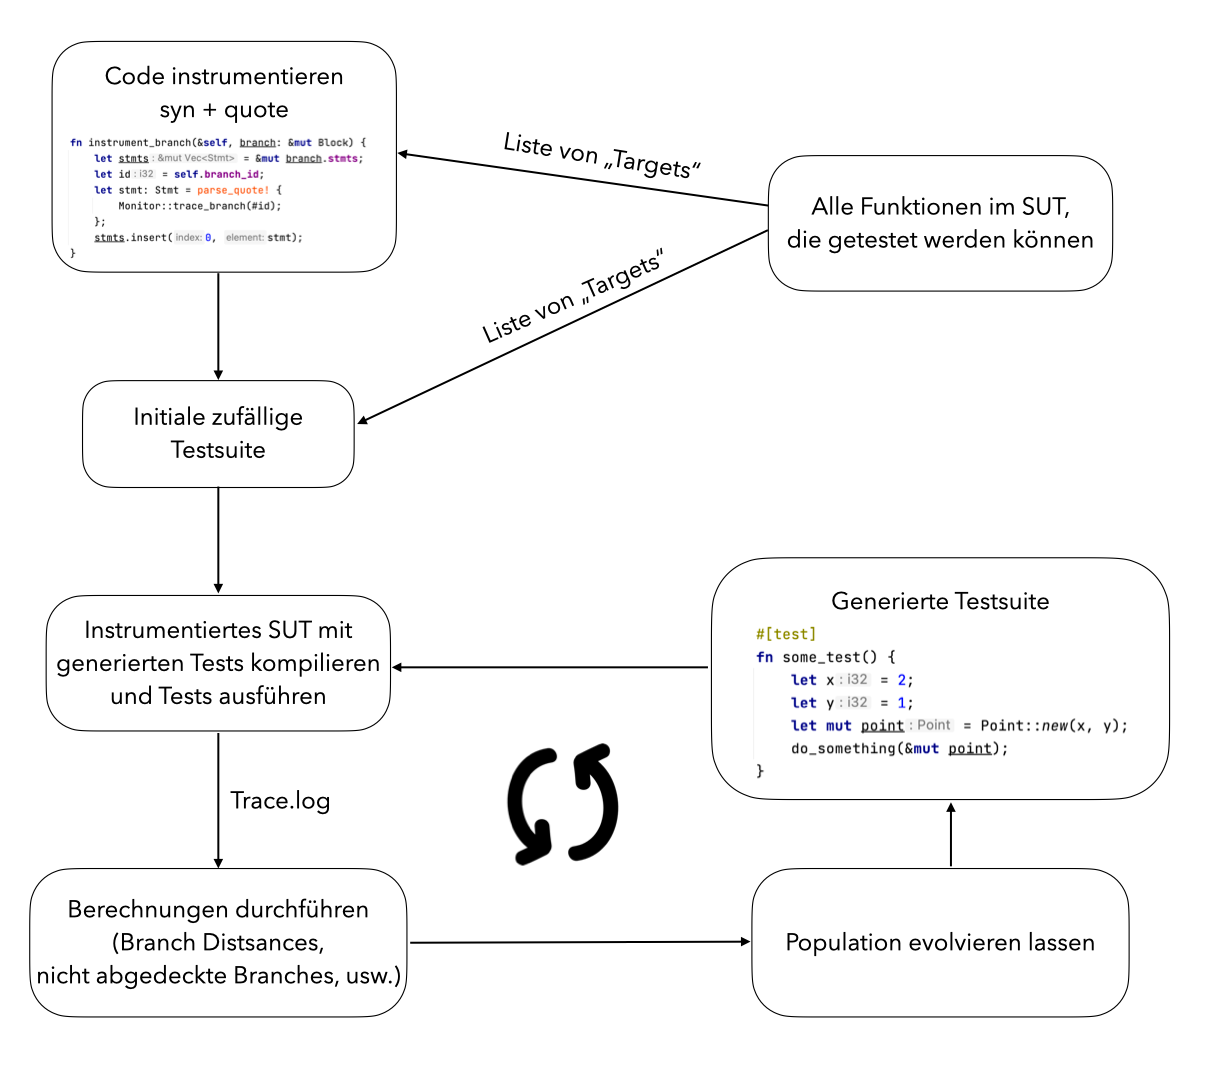
\includegraphics[width=\textwidth]{old-overview}
%\label{fig:old-overview}
%\end{figure}

\section{Instrumentation}
Tests that are generated by a search-based technique need to be executed at least once to provide some feedback on their fitness in regard to the \ac{SUT}. At this point, the coverage data and branch distances can be collected. In order to do so, the \ac{SUT} has to be instrumented with additional code, which traces the executed paths. Many other state of the art tools that generate coverage for Java instrument the bytecode of the compiled \ac{SUT} and use Reflection to run the generated tests. However, Rust compiles to machine code. Although there exist tools that allow static analysis and binary transformation, e.g., reg.ng~\cite{DiFederico2018}, the instrumentation will be done on the source code level. \textbf{syn} and \textbf{quote} are two mature libraries that allow parsing Rust code into a syntax tree and converting the tree back to regular code, respectively.

During the instrumentation, additional tracing statements will be inserted into a \ac{SUT} to report visited branches. The original source files will be backed up and temporarily replaced by the instrumented ones. Additionally, while traversing the syntax tree, all testable data structures, as well as their constructors, fields, and methods, are captured. At the end of this process, it will be known which methods can be tested, what parameters they have, which generators can be used to instantiate those parameters, and how the parameters are used, i.e., borrowed or consumed.

\begin{lstlisting}[style=boxed, caption=Division by zero transformation, label=lst:example-testability-transformation]
fn div(a: i32, b: i32) -> f64 {
    if b == 0 {
        panic!("Dividing by zero")
    } else {
        a as f64 / b as f64
    }
}
\end{lstlisting}

Similar to Java, trait implementations in Rust must follow some standard contracts. For instance, when implementing both \texttt{Hash} and \texttt{Eq}, it is required that the following property holds:
\[
k1 == k2 \longrightarrow hash(k1) == hash(k2)
\]
i.e., if two keys are equal, their hashes must also be equal. Some of the traits in the standard library can be derived automatically, which should generate implementations that comply with an appropriate contract. However, a manual implementation might still be desirable in case some members of a struct do not implement the trait to derive, or a custom version is required. A contract violation might be considered a bug and shall be checked during the execution of generated tests, as is done in \textsc{Randoop}~\cite{Pacheco_2007} and \textsc{EvoSuite}~\cite{Fraser2013}.

\section{Test Execution}
With Cargo, Rust provides a build system and a testing framework out-of-the-box. In Java, which is a managed language~\cite{Gough2005}, generated tests can be executed directly using Reflection and bytecode instrumentation, and coverage information can be collected in the same runtime process. This cannot be done that conveniently in Rust, and tests must first be compiled. Then the Cargo test framework is called on the module under test to run the tests. To speed up the process, a whole population of tests is compiled and run concurrently. To keep the exact coverage of each individual test, each test sets a \texttt{thread\string_local} test ID at the beginning of its execution, which the instrumented \ac{SUT} uses during execution to trace the coverage.

As shown in \Cref{fig:test-execution}, the instrumented \ac{SUT} reports important events during its execution to the message queue of the monitor thread (MT). These are, for example, the execution of a root branch (method or function) or a decision branch. For the latter, the branch distance, which is calculated on the fly, is passed along with other data. The MT is initialized before the threads are started and can either write collected coverage data to a file or send it directly to the main process via \ac{TCP}.

\begin{figure}[h]
\caption{An example concurrent execution of multiple tests with a monitor}
\centering
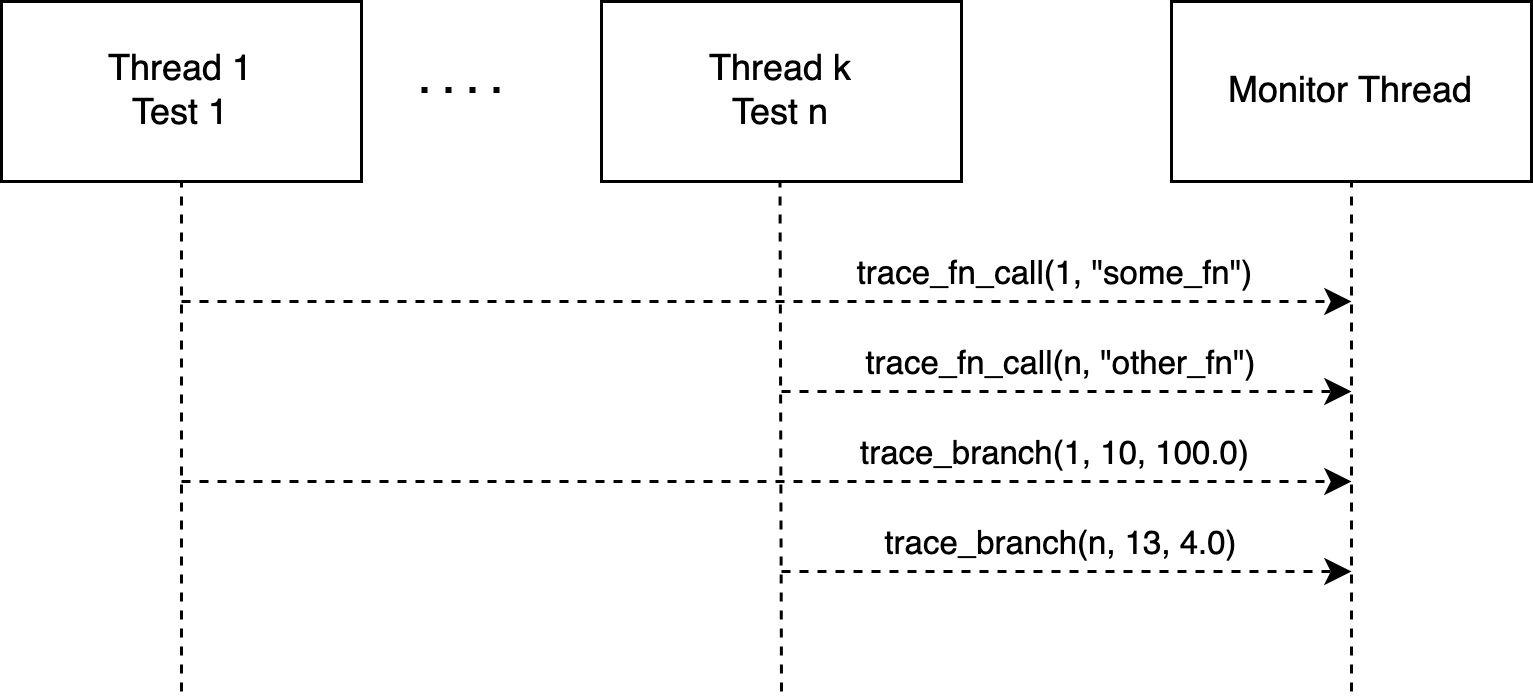
\includegraphics[width=\textwidth]{test-execution}
\label{fig:test-execution}
\end{figure}

Real and complex software often interacts with its environment, for example by making I/O calls to the file system or establishing \ac{TCP} connections. Lack of handling of the execution environment the \ac{SUT} lives within is still one of the open problems in \ac{SBST}~\cite{McMinn2011}. To avoid unwanted side effects, \textsc{EvoSuite}~\cite{Fraser2013a} relies on strict security measures of the Java Security Manager and prohibits most interactions of \ac{SUT} with its environments. These could lead to uncontrolled behavior if executed repeatedly, such as generating countless random files or even wiping the entire disk. Only few essential operations are allowed, such as I/O for the classloader, loading libraries, or reflection. As a preprocessing step, \textsc{EvoSuite} extracts only those methods that return the same result when run repeatedly with the same inputs, i.e., methods that are deterministic~\cite{Fraser2012}.

\textsc{KLEE}~\cite{cadar2008klee} takes a different approach and redirects concrete calls, such as \texttt{open()} and \texttt{read()}, to \textit{models} that understand the semantics of the desired action well enough to generate the required constraints. These models are written in normal C code which the use can readily customize, extend, or even replace with their own custom implementation. Function calls are replaced in a pre-processing step in \ac{SUT} by mocks that mimic the original behavior. When the \ac{SUT} reads values from the environment, such as from a file, a legal, randomly generated value of the same type is returned as the original function would have done. When the \ac{SUT} writes to the environment, the values are stored in memory during the execution of the corresponding test such that the effect of these alterations are reflected in potential subsequent reads.


\section{Test Suite Optimization}
~\Cref{fig:old-overview} illustrates the main steps in the tool: it starts by instrumenting the \ac{SUT} and inserting necessary statements to trace a programm execution. Then, a random test suite is generated based on the \ac{SUT} and evolved using evolutionary search towards a specified fitness goal. At the end, the test suite with the highest coverage is returned.

\subsection{Problem representation}
\label{sec:problem-representation}
According to McMinn~\cite{McMinn_2004}, an encoding of the solution should be modeled in a way that similar solutions are also neighbors in the represented search space. This makes it easy to continue the search from one to a similar solution by applying simple modifications of the representation. In single-objective genetic algorithms for test generation, a chromosome in a population typically represents an entire test suite~\cite{Fraser_2011a, Campos2017}. However, \acp{MOA} define a chromosome to be a single test case~\cite{Panichella2018}. Chromosome representation has a direct impact on how, for instance, the crossover operator works. Recombining two test suites is trivial by recombining only the sequences of their test cases at specific cut points since individual test cases are independent of each other~\cite{Fraser_2013}. Recombining test cases is more complicated because it means recombining their sequences of statements, which are, however, very much interdependent. For example, a statement could instantiate an object by invoking an appropriate constructor, followed by a later method invocation on that object. In the following, a chromosome is a test case, which is a sequence of statements or program calls that execute parts of the \ac{SUT} to reach and cover a certain objective. Since programs in Rust are not just procedures but have a certain class-like structure, this must also be taken into account. In a simple procedural program, tests would only need to call procedures with certain input data to achieve high coverage. However, instances of structs can have states that can be changed either directly or via method calls. The control flow graph of a method may depend on the internal state of an object. This means that a certain statement call sequence may be important to achieve high code coverage. For the generation of unit tests with a genetic algorithm, this work implements already known ideas for the representations of genetic solutions~\cite{Fraser2012,Tonella2004,Arcuri2008}. Similar to Frasers and Arcuris~\cite{Fraser_2011a} definition, each statement~$s_i$ in a test case is a value~$v(s_i)$, which has a type~$\tau(v(s_i)) \in \mathcal{T}$, where~$\mathcal{T}$ is the finite set of types. There can be five different types of statements:

\begin{itemize}
    \item \textbf{Primitive statements} represent numeric variables, e.g., \texttt{let v = 42}. Value and type of the statement are defined by the primitive variable.
    \item \textbf{Constructor statements} generate new instances of a given struct, z. B. \texttt{let b = Book::new()}. Value and type of the statement are defined by the object constructed in the call. A constructor can have parameters whose values are assigned out of the set ~$\{v(s_k)~|~0 \leq k < i\}$. However, constructors are not part of the Rust language. Using a static method called \texttt{new}, which returns an instance of the appropriate struct, is not mandatory but a convention. Thus, if a struct does not provide the new method, it still can be instantiated the C-like way, i.e., \texttt{let b = Book \string{ name: "A" \string}}.
    \item \textbf{Field statements} access member variables of objects, e.g., \texttt{let b = a.x}. Value and type of a field statement are defined by the member variable. The source of the member variable, i.e.,~\texttt{a}, must be part of the set~$\{v(s_k)~|~0 \leq k < i\}$. Since unit tests are usually contained in the same module as the~\ac{CUT}, tests can also legally access private fields.
    \item \textbf{Method statements} invoke associative methods on objects or static methods, e.g., \texttt{let b = a.len()}. The owner of the method (if non-static) and all of the parameters must be values in~${\{v(s_k)~|~0 \leq k < i\}}$. Value and type of a method statement are defined by its return value.
    \item \textbf{Function statements} invoke free-standing functions, e.g., \texttt{let a = foo()}. The parameters of the function must be values in~$\{v(s_k)~|~0 \leq k < i\}$. Value and type of a function statement are defined by its return value.
\end{itemize}

The collection of available structs, their constructors, methods, fields, and free-standing functions are so-called test cluster~\cite{Fraser_2011a}. The size of a test suite as well as individual tests is dynamic and can change (almost) arbitrarily. Since there will be no test oracles available for most of the generated tests, the size of the test suite, as well as the individual tests, should have an upper limit, so that test oracles can be inserted later manually. Of course, it also makes sense not to let a test become completely blank.

Each statement that does not have the default return value~\texttt{()} defines a new variable. However, a generated test cannot be composed arbitrarily of the above building blocks. Each test is subject to the same constraints as regular Rust programs, which are checked by the compiler~\cite{Tonella2004}. Constructors, methods, functions, and fields in a test are not limited to just the parts of the module under the test since complex sequences of calls might be necessary to define some arguments~\cite{Fraser2012}.

Rust's affine type system makes usage of already defined objects more complicated since the information in which statements a particular instance was used in which way (borrowed or consumed) must also be tracked. That is, an already defined object may be used in any way by a newly inserted statement~$s'$ only if it is marked as free to use and is not used by any other statement~$s$ that comes after~$s'$. Otherwise,~$s'$ may use the object in a way that does not collide with~$s$. More precisely, the rules are defined as follows: let~$t$ be a test case and $pos(s)$ a function that returns the position of a statement~$s$ in the sequence of statements in~$t$. Let~$o$ be an object of a data type~$\tau(o)$ defined by statement~$gen$. A new statement~$s'$ is inserted, which uses~$o$. Then the following must hold:
\begin{itemize}
    \item $gen \in t \wedge pos(gen) < pos(s')$.
    \item If~$o$ is not used by any statement~$s \in t$,~$o$ may be consumed or borrowed by~$s'$.
    \item If~$o$ is borrowed by a statement~$s \in t$,~$o$ may also be borrowed by~$s'$ at position~$p_{borrow}$ with ~$pos(gen) < p_{borrow}$ or consumed at position~$p_{consume}$ with~$pos(s) < p_{consume} < \left|t\right|$.
    \item If~$o$ is consumed by a statement~$s \in t$,~$o$ may be borrowed by~$s'$ at position~$p_{borrow}$ with~$pos(gen) < p_{borrow} < pos(s)$.
\end{itemize}

%Fraser und Zeller~\cite{Fraser2012} beschreiben in ihrer Arbeit zum Mutations-basiertem Generieren von Tests für Java Klassen ein abstraktes Konstrukt, welches die Modellierung und Aufbau eines Unit Tests leicht veranschaulicht. Sei~$parameters(M)$ eine Funktion, die eine Liste von Datentypen der Parameter einer Methode oder Funktion~$M$ zurückgibt, einschließlich des Aufrufers im Falle einer nicht-statischen Methode. Des Weiteren, sei~$classes(t)$ eine Funktion, die den Set von Datentypen zurückgibt, dessen Objekte in einem Test~$t$ bereits instanziert wurden. Eine Funktion oder eine Methode ist ein Generator eines Datentyps~$C$ wenn sie einen Rückgabewert vom Typ~$C$ haben. Außerdem ist jeder Konstruktor eines Structs vom Typ~$C$ ebenfalls ein Generator von~$C$. Sei~$generators(M,C)$ eine Funktion, die den Set von Generatoren für den Datentyp~$C$ aus dem Set von Methoden und Funktionen~$M$ zurückgibt.

Fraser and Zeller~\cite{Fraser2012} describe in their work on mutation-based generation of tests for Java classes an abstract construct that easily illustrates the modeling and construction of a unit test. Let~$parameters(M)$ be a function that returns a list of data types of the parameters of a method or function~$M$, including the caller in the case of a non-static method. Furthermore, let~$classes(t)$ be a function that returns the set of data types whose objects have already been instantiated in a test~$t$. A function or a method is a generator of a datatype~$C$ if they have a return value of type~$C$. Furthermore, any constructor of a struct of type~$C$ is also a generator of~$C$. Let~$generators(M,C)$ be a function that returns the set of generators for the data type~$C$ from the set of methods and functions~$M$.

\begin{algorithm}[t]
\caption{$GenTest(M, l)$}\label{alg:random-generation-of-a-test}
\begin{algorithmic}
\Input
  \Desc{$M$}{Set of all method, constructors and functions}
  \Desc{$l$}{Desired length of a test case}
\EndInput
\Output
  \Desc{$t$}{Randomly generated test}
\EndOutput
\State{$t \gets \langle\rangle$}
\State{$s \gets$ randomly select an element from M}


\For{$p \in parameters(s)$}
  \State{$t \gets GenObject(p, \{\}, M, t)$}
\EndFor
\State{$t \gets t.s$}

\While{$\left|t\right| < l$}
  \State{$c \gets$ randomly select datatype in $classes(t)$}
  \State{$M' \gets \{m | m \in M \wedge c \in parameters(m)\}$}
  \State{$s \gets$ randomly select method or function from $M'$}
  \For{$p \in parameters(s)$}
    \If{$\neg(p \in classes(t))$}
      \State{$t \gets GenObject(p, \{\}, M, t)$}
    \EndIf
  \EndFor
  \State{$s \gets$ set parameters of $s$ to values from $t$}
  \State{$t \gets t.s$}
\EndWhile
\State \Return $t$
\end{algorithmic}
\end{algorithm}


% Die initiale Population wird zufällig generiert, wie im Algorithmus~\labelcref{alg:random-generation-of-a-test} dargestellt. Bevor die Tests generiert werden, werden alle verfügbaren Methoden, Konstruktoren und Funktionen, sowie Attribute von Structs statisch aus der \ac{HIR} des \ac{SUT} extrahiert. Bei einem zufällig generierten Test wird daraus ein zufälliger Aufruf eingefügt. Die evtl. notwendigen Argumente (ggf. inklusive des Aufrufers, das heißt des Methodeninhabers) werden dabei ebenfalls generiert. Dafür werden entsprechende Aufrufe, die Rückgabewerte von passenden Datentypen haben, rekursiv eingefügt (Algorithmus~\labelcref{alg:genobject}), wenn im Test Case nicht bereits Instanzen eines solchen Datentyps definiert und entsprechend den Regeln aus \Cref{sec:problem-representation} verwendbar sind. Während der Suche werden die Datentypen, die zu instanziieren bereits versucht wird, gemerkt, um unendliche Rekursionen zu vermeiden. Laut den Algorithmen~\labelcref{alg:random-generation-of-a-test} und~\labelcref{alg:genobject} werden neue Objekte nur dann generiert, wenn sie nicht im Test bereits existieren. Fraser und Zeller~\cite{Fraser2012} schlagen jedoch vor, bestehende Objekte nur mit einer gewissen Wahrscheinlichkeit wiederzuverwenden, um Diversität in generierten Test Cases zu erhöhen. In ihren Experimenten haben sie festgestellt, dass eine Wahrscheinlichkeit von 90\% Prozent am effektivsten ist. Rust's affines Typsystem macht eine Wiederverwendung von bereits definierten Objekten komplizierter, da es analysiert werden muss, inwieweit eine bestimmte Variable in einem gegebenen Test noch verwendbar ist. Das heißt, dass eine bereits definierte Variable nur dann von einem neu eingefügten Statement~$s$ verwendet werden darf, wenn sie als frei verwendbar markiert. \todo{Das gilt nicht für Typen, die Copy implementieren}Genauer werden die Regeln folgenderweise definiert: Sei~$t$ ein Test Case und $pos(s)$ eine Funktion, die die Position eines Statements~$s$ in der Sequenz der Statements von~$t$ zurückgibt. Sei~$o$ eine Objekt, das von einem Statement~$gen$ definiert wird. Sei~$s$ ein Statement, welches~$o$ verwendet. Dann ist $t$ nur in dem Fall ein valider Test Case, wenn folgende Regeln eingehalten werden:

The initial population is randomly generated as shown in the \Cref{alg:random-generation-of-a-test}. Before the tests are generated, all available methods, constructors and functions, as well as attributes of structs are statically extracted from the \ac{HIR} of the \ac{SUT}. For a randomly generated test, a random call is inserted from this. The possibly necessary arguments (including the caller, i.e. the method owner, if applicable) are also generated during the process. To this end, corresponding calls that have return values of suitable data types are inserted recursively (algorithm~\labelcref{alg:genobject}), if instances of such a data type are not already defined in the test case and usable according to the rules from \Cref{sec:problem-representation}. During the search, the data types that are already attempted to be instantiated are remembered to avoid infinite recursion. According to the \Cref{alg:random-generation-of-a-test, alg:genobject}, new objects are generated only if they do not already exist in the test. However, Fraser and Zeller~\cite{Fraser2012} suggest reusing existing objects only with a certain probability to increase diversity in generated test cases. In their experiments, they found that a probability of 90\% percent was most effective. Rust's affine type system makes reuse of previously defined objects more complicated because it requires analysis of the extent to which a given variable is still usable in a given test. This means that an already defined variable may only be used by a newly inserted statement~$s$ if it is marked as freely usable. More precisely, the rules are defined as follows: let~$t$ be a test case and $pos(s)$ be a function that returns the position of a statement~$s$ in the sequence of statements of~$t$. Let~$o$ be an object defined by a statement~$gen$. Let~$s$ be a statement that uses~$o$. Then $t$ is a valid test case only if the following rules are satisfied:

\begin{itemize}
    \item $pos(gen) < pos(s)$, AND
    \item if $o$ is not used by any statement $s' \in t$,~$o$ may be freely consumed and borrowed by~$s$, AND
    \item if $o$ is borrowed from a statement~$s' \in t$, $o$ may also be borrowed from $s$ at position $p_{borrow}$ with $pos(gen) < p_{borrow}$ or consumed at position $p_{consume}$ with $pos(s') < p_{consume} < \left|t\right|$, AND
    \item if $o$ is consumed by a statement $s' \in t$, $o$ may now be borrowed only from $s'$ at position~$p_{borrow}$ with $pos(gen) < p_{borrow} < pos(s)$.
\end{itemize}

These rules must also be strictly followed when using search operators during the search, so that the generated test cases represent correct Rust code. The rules also cover edge cases, such as multiple consumption of a variable from a statement, as shown in the following non-valid test case (when \texttt{A} does not implement \texttt{Copy}):
\begin{lstlisting}[style=boxed, caption={}]
let a = A::new();
let pair: Pair<A, A> = Pair::of(a, a);
\end{lstlisting}

We adopt the \Cref{alg:genobject} from Fraser and Zeller and use it to try to generate dependencies of methods and functions. Since we do not perform a complete analysis of all possible types, it may happen that \texttt{GenObject} fails the search and cannot generate an object of the appropriate type. In this case, we skip the particular method or function for which we tried to generate the argument. Of course, this leads to worse coverage results, but a complete analysis of all possible cases is not easy and cannot be done within the scope of this work.

\begin{algorithm}[t]
\caption{$GenObject(c, G, M, t)$}
\label{alg:genobject}
\begin{algorithmic}
\Input
  \Desc{$c$}{Datatype of desired object}
  \Desc{$G$}{Set of datatypes already attempting to generate}
  \Desc{$M$}{Set of all method, constructors and functions}
  \Desc{$t$}{Test case}
\EndInput
\Output
  \Desc{$t$}{Test case extended with an instance of $c$}
\EndOutput
\State{$M' \gets generators(M, c)$}
\State{$s \gets$ randomly select an element from M'}

\For{$c \in parameters(s)$}
  \If{$\neg(c \in classes(t))$}
    \State{$t \gets GenObject(c, G, M, t)$}
  \EndIf
\EndFor
\State{$s \gets$ set parameters of $s$ to values from $t$}
\State{$t \gets t.s$}
\State \Return $t$
\end{algorithmic}
\end{algorithm}

\subsection{Search Operators}
\label{sec:search-operators}
The evolution of a population is performed by repeated selection of test cases and applying crossover and mutation operators according to a certain probability~\cite{Fraser2012}.

There are different selection methods, e.g., fitness-proportional selection, linear ranking, or tournament selection~\cite{McMinn_2004}. The key is to guide the search towards solutions with better fitness values. Once the set of parents has been selected, recombination (or crossover) can take place to form the next generation. Crossover is applied to individuals with a certain probability. The most basic recombination is a single point crossover, where a random position in each of the two selected test cases is selected, and new test cases (offspring) are generated by swapping the subsequences of statements~\cite{Fraser2012}. At this point, the dependencies, i.e., arguments, of the statements will be considered, and possibly missing arguments will be generated in the offspring test cases.

After selection and crossover have been applied, the offspring can mutate. There are different ways of mutating a sequence-based test case, e.g., delete, insert, or modify a statement~\cite{Fraser2012}. Modifying a statement includes changing the callee of a method, parameters, or replacing the method itself with another one. The rules defined in \Cref{sec:problem-representation} determine when the offspring is valid with respect to Rust compiler, e.g., replacing a method call\texttt{fn foo(\string&self)} by \texttt{fn bar(self)} is not allowed if the callee of the method, i.e., the variable, is also used by another statement in some way later in the sequence because the \texttt{bar} method consumes the callee.

\subsection{Mutation}
Da Chromosome werden in ihrer ''natürlichen'' Weise repräsentiert werden, und ein Test Case somit aus einer Sequenz von Statements besteht, muss der Mutationsoperator entsprechend definiert werden. Wir adoptieren die Definition der Mutation für Sequenz-basierte Repräsentation der Test Cases von Fraser und Arcuri~\cite{Fraser2012}. Demnach kann eine Mutation folgende Ausprägungen haben:
\begin{description}
  \item[Insert a statement] A given test case $t$ is extended with a probability $\sigma$ by a new statement, which is inserted at a random position in $t$. A new statement can only be inserted if $l(t) < L$, i.e. if the test length does not exceed a defined maximum. For each insertion, with probability $1/3$ a random call out of the pool of callables is inserted, with probability $1/3$ a method call on a value in the set $\{v(s_k) \left| 0 \leq k < i \right\}$ is used as a parameter in a random call. Any parameters of the selected call are either reused out of the set $\{v(s_k) \left| 0 \leq k < i \right\}$ or randomly generated. Each parameter~$p$ selected from $\{v(s_k) \left| 0 \leq k < i \right\}$ must be usable by the call according to the rules in \Cref{sec:problem-representation}. The random position of the new statement must be at least greater than $max(\{pos_t(a) : a \text{ is an argument of } c\})$ or greater than or equal to $0$ if~$c$ has no parameters. Multiple statements can also be inserted repeatedly, where this happens with probability~$p(n) = 0.5^n$, where~$n$ is the number of calls inserted so far. That is, after each insertion, a random decision is made whether to repeat the mutation~\cite{Tonella2004}. An example in \Cref{lst:mutation-invocation-insertion} demonstrates how two additional method calls \texttt{push} and \texttt{len} on an existing vector instance have been inserted. 

  \begin{lstlisting}[style=boxed, caption=, label=lst:mutation-invocation-insertion, caption={Two methods, \textit{push} (line 18) and \textit{len} (line 19) have been selected randomly to be inserted on \textit{vec\string_0}. An appropriate argument has been generated for the second \textit{push}, too}]
  #[test]
  fn test() {
    let usize_0 = 32;
    let mut vec_0 = Vec::with_capacity(usize_0);
    let i32_0 = 45;
    vec_0.push(i32_0);
  }

  // became

  #[test]
  fn test() {
    let usize_0 = 32;
    let mut vec_0 = Vec::with_capacity(usize_0);
    let i32_0 = 45;
    vec_0.push(i32_0);
    let i32_1 = 106;
    vec_0.push(i32_1);
    let usize_1 = vec_0.len();
  }
  \end{lstlisting}

  \item[Change a statement] For a test case $t = (s_1, s_2, \dots, s_l)$ with length~$l$, each statement~$s_i$ is changed with probability $1/n$. If $s_i$ is a primitive statement, then the numeric value represented by $s_i$ is changed by a random value in $\pm[0,\Delta]$ where $\Delta$ is a constant. If $s_i$ is not a primitive statement, then either a method, function, or a field with the same return type as $v(s_i)$ and parameters satisfiable with the values in the set $\{v(s_k) \left| 0 \leq k < i \right\}$ is randomly chosen or the arguments $a_1, \dots, a_n$ of $s_i$ are changed with the probability $1/n$. Each changed argument $a_x$ is replaced by a random value out of the set $\{v(s_k) \left| 0 \leq k < l \right\}$ or a generated value. The new value must again satisfy the rules defined in \Cref{sec:problem-representation}. In \Cref{lst:mutation-input-value}, the first argument (vector instance) of the method call \texttt{push} was replaced by another one, which was generated on-the-fly because no other instance of the same type existed in the test before.

  \begin{lstlisting}[style=boxed, label=lst:mutation-input-value, caption={The first argument (which effectively is the method owner) of the call to \textit{push} (line 8) has been changed to a newly created value \textit{vec\string_1}}]
  #[test]
  fn test() {
    let usize_0 = 32;
    mut vec_0 = Vec::with_capacity(usize_0);
    let i32_0 = 45;
    vec_0.push(i32_0);
    let i32_1 = 106;
    vec_0.push(i32_1);
    let usize_1 = vec_0.len();
  }

  // became

  #[test]
  fn test() {
    let usize_0 = 32;
    let mut vec_0 = Vec::with_capacity(usize_0);
    let i32_0 = 45;
    vec_0.push(i32_0);
    let i32_1 = 106;
    let mut vec_1 = Vec::new();
    vec_1.push(i32_1);
    let usize_1 = vec_0.len();
  }
  \end{lstlisting}

  \item[Delete a statement] For a test case $t = (s_1, s_2, \dots, s_l)$ with length~$l$, each statement~$s_i$ can be deleted with probability~$1/l$. As the value $v(s_i)$ might be used as an argument in any of the statements $s_{i+1}, \dots, s_l$, the test needs to be repaired to remain valid. For each statement $s_j$, $i < j \leq l$, if $s_j$ refers to $v(s_i)$, then this argument is replaced with another value out of the set $\{v(s_k) \left| 0 \leq k < j \wedge k \neq i \right\}$ which has the same type as $v(s_i)$ and is allowed to be used according to the rules from \Cref{sec:problem-representation}. If this is not possible, then $s_j$ is deleted as well recursively~\cite{Fraser2012}. In \Cref{lst:mutation-invocation-removal}, an instance of a vector was deleted, affecting the method calls on that instance as well. For the \texttt{push} method call, there is no alternative instance of the same type. Since it does not return any value, it can simply be eliminated because no other statements make use of it. The call to the \texttt{len} method was transferred to the other instance of the same type present in the test (\texttt{vec\string_1}). If there were no second instance of the same type in the test, or it was already consumed at this point, the statement would be have been removed, too.

  \begin{lstlisting}[style=boxed, caption=, label=lst:mutation-invocation-removal, caption={The definition of \textit{vec\string_0} has been deleted, and statements that used it have been updated}]
  #[test]
  fn test() {
    let usize_0 = 32;
    let mut vec_0 = Vec::with_capacity(usize_0);
    let i32_0 = 45;
    vec_0.push(i32_0);
    let i32_1 = 106;
    let mut vec_1 = Vec::new();
    vec_1.push(i32_1);
    let usize_1 = vec_0.len();
  }

  // became

  #[test]
  fn test() {
    let usize_0 = 32;
    let i32_0 = 45;
    let i32_1 = 106;
    let mut vec_1 = Vec::new();
    vec_1.push(i32_1);
    let usize_1 = vec_1.len();
  }
  \end{lstlisting}
  %The call to \texttt{a.f(b)} was randomly selected for deletion. Since it was the only place where \texttt{b} was used, it was also deleted. Similar to inserting method calls, this operator can be applied repeatedly with probability~$p(n) = 0.5^n$, where $n$ is the number of deleted statements.

\end{description}


\subsection{Crossover}
%Die einfachste Art von Crossover ist der One-Point-Crossover, so wie er in~\Cref{sec:background-crossover} beschrieben ist. Die Chromosome werden hier jedoch in der natürlichen Art repräsentiert, als Sequenz von Statements, was dazu führt, dass beim Aufteilen und Durchtauschen von Köpfen eines Paars von Chromosomen auf die Abhängigkeiten zwischen einzelnen Statements geachtet werden muss. Zum Beispiel besteht eine Abhängigkeit zwischen einem Methodenaufruf und seinen Argumenten, die wir in einem Test immer in einem eigenen Statement initialisieren. Wenn der Schnittpunkt einer Rekombination so eine Abhängigkeit zwischen Statements trifft, werden die so neu geschaffenen rekombinierten Test Cases in den meisten Fällen nicht vom Compiler akzeptiert. Tonella~\cite{Tonella2004} hat für dieses Problem zwei Lösungen vorgeschlagen:

The simplest type of crossover is the one-point crossover, as described in~\Cref{sec:background-crossover}. However, the chromosomes here are represented in the natural way, as a sequence of statements, which means that when splitting and swapping heads of a pair of chromosomes, attention must be paid to the dependencies between individual statements. For example, there is a dependency between a method call and its arguments, which we always initialize in a separate statement in a test. If the intersection of a recombination hits such a dependency between statements, the newly created recombined test cases will not be accepted by the compiler in most cases. Tonella~\cite{Tonella2004} has proposed two solutions to this problem:

\begin{itemize}
    \item Missing dependencies of statements can be added by generating, as with the mutation operator. If certain definitions become redundant because their later use has been pushed into another choromosome by recombination, they can be deleted.
    \item Dependencies from a part of a chromosome shifted by recombination are also shifted to another chromosome regardless of the crossover point, provided they are no longer needed in the original chromosome, otherwise they could be copied.
\end{itemize}

% Bei der Rekombination setzen wir auf die erste Option: Im Fall, dass Argumente eines rekombinierten Test Cases außenvor bleiben, generieren wir diese nachträglich mittels des \texttt{GenObject} Algorithmus, sodass der Test Case wieder kompilierbar wird. In \Cref{fig:crossover-example} wird ein solcher Fall veranschaulicht. Es wird ein zufälliger Schnittpunkt in den beiden Test Cases blau und grün bestimmt. Durch Rekombination der Statements entstehen zwei neue Test Cases, die beide jedoch in der Form nicht kompilierbar sind, da sowohl im linken (\texttt{hashmap_0}) als auch im rechten Test Case (\texttt{f64_0}) Instanzen verwendet werden, die in den jeweiligen Tests gar nicht definiert sind. Aus diesem Grund müssen wir einen Repair-Schritt durchführen und fehlende Abhängigkeit generieren (in rot).

For recombination, we rely on the first option: in the case that arguments of a recombined test case are left out, we generate them afterwards using the \texttt{GenObject} algorithm, so that the test case becomes compilable again. In \Cref{fig:crossover-example} such a case is illustrated. A random intersection in the two test cases blue and green is determined. By recombining the statements, two new test cases are created, both of which, however, cannot be compiled in the form, since both the left (\texttt{hashmap\string_0}) and the right test case (\texttt{f64\string_0}) use instances that are not defined in the respective tests at all. For this reason, we need to perform a repair step and generate missing dependency (in red).

\begin{figure}[h]
\caption{Crossover between two test cases with postprocessing}
\centering
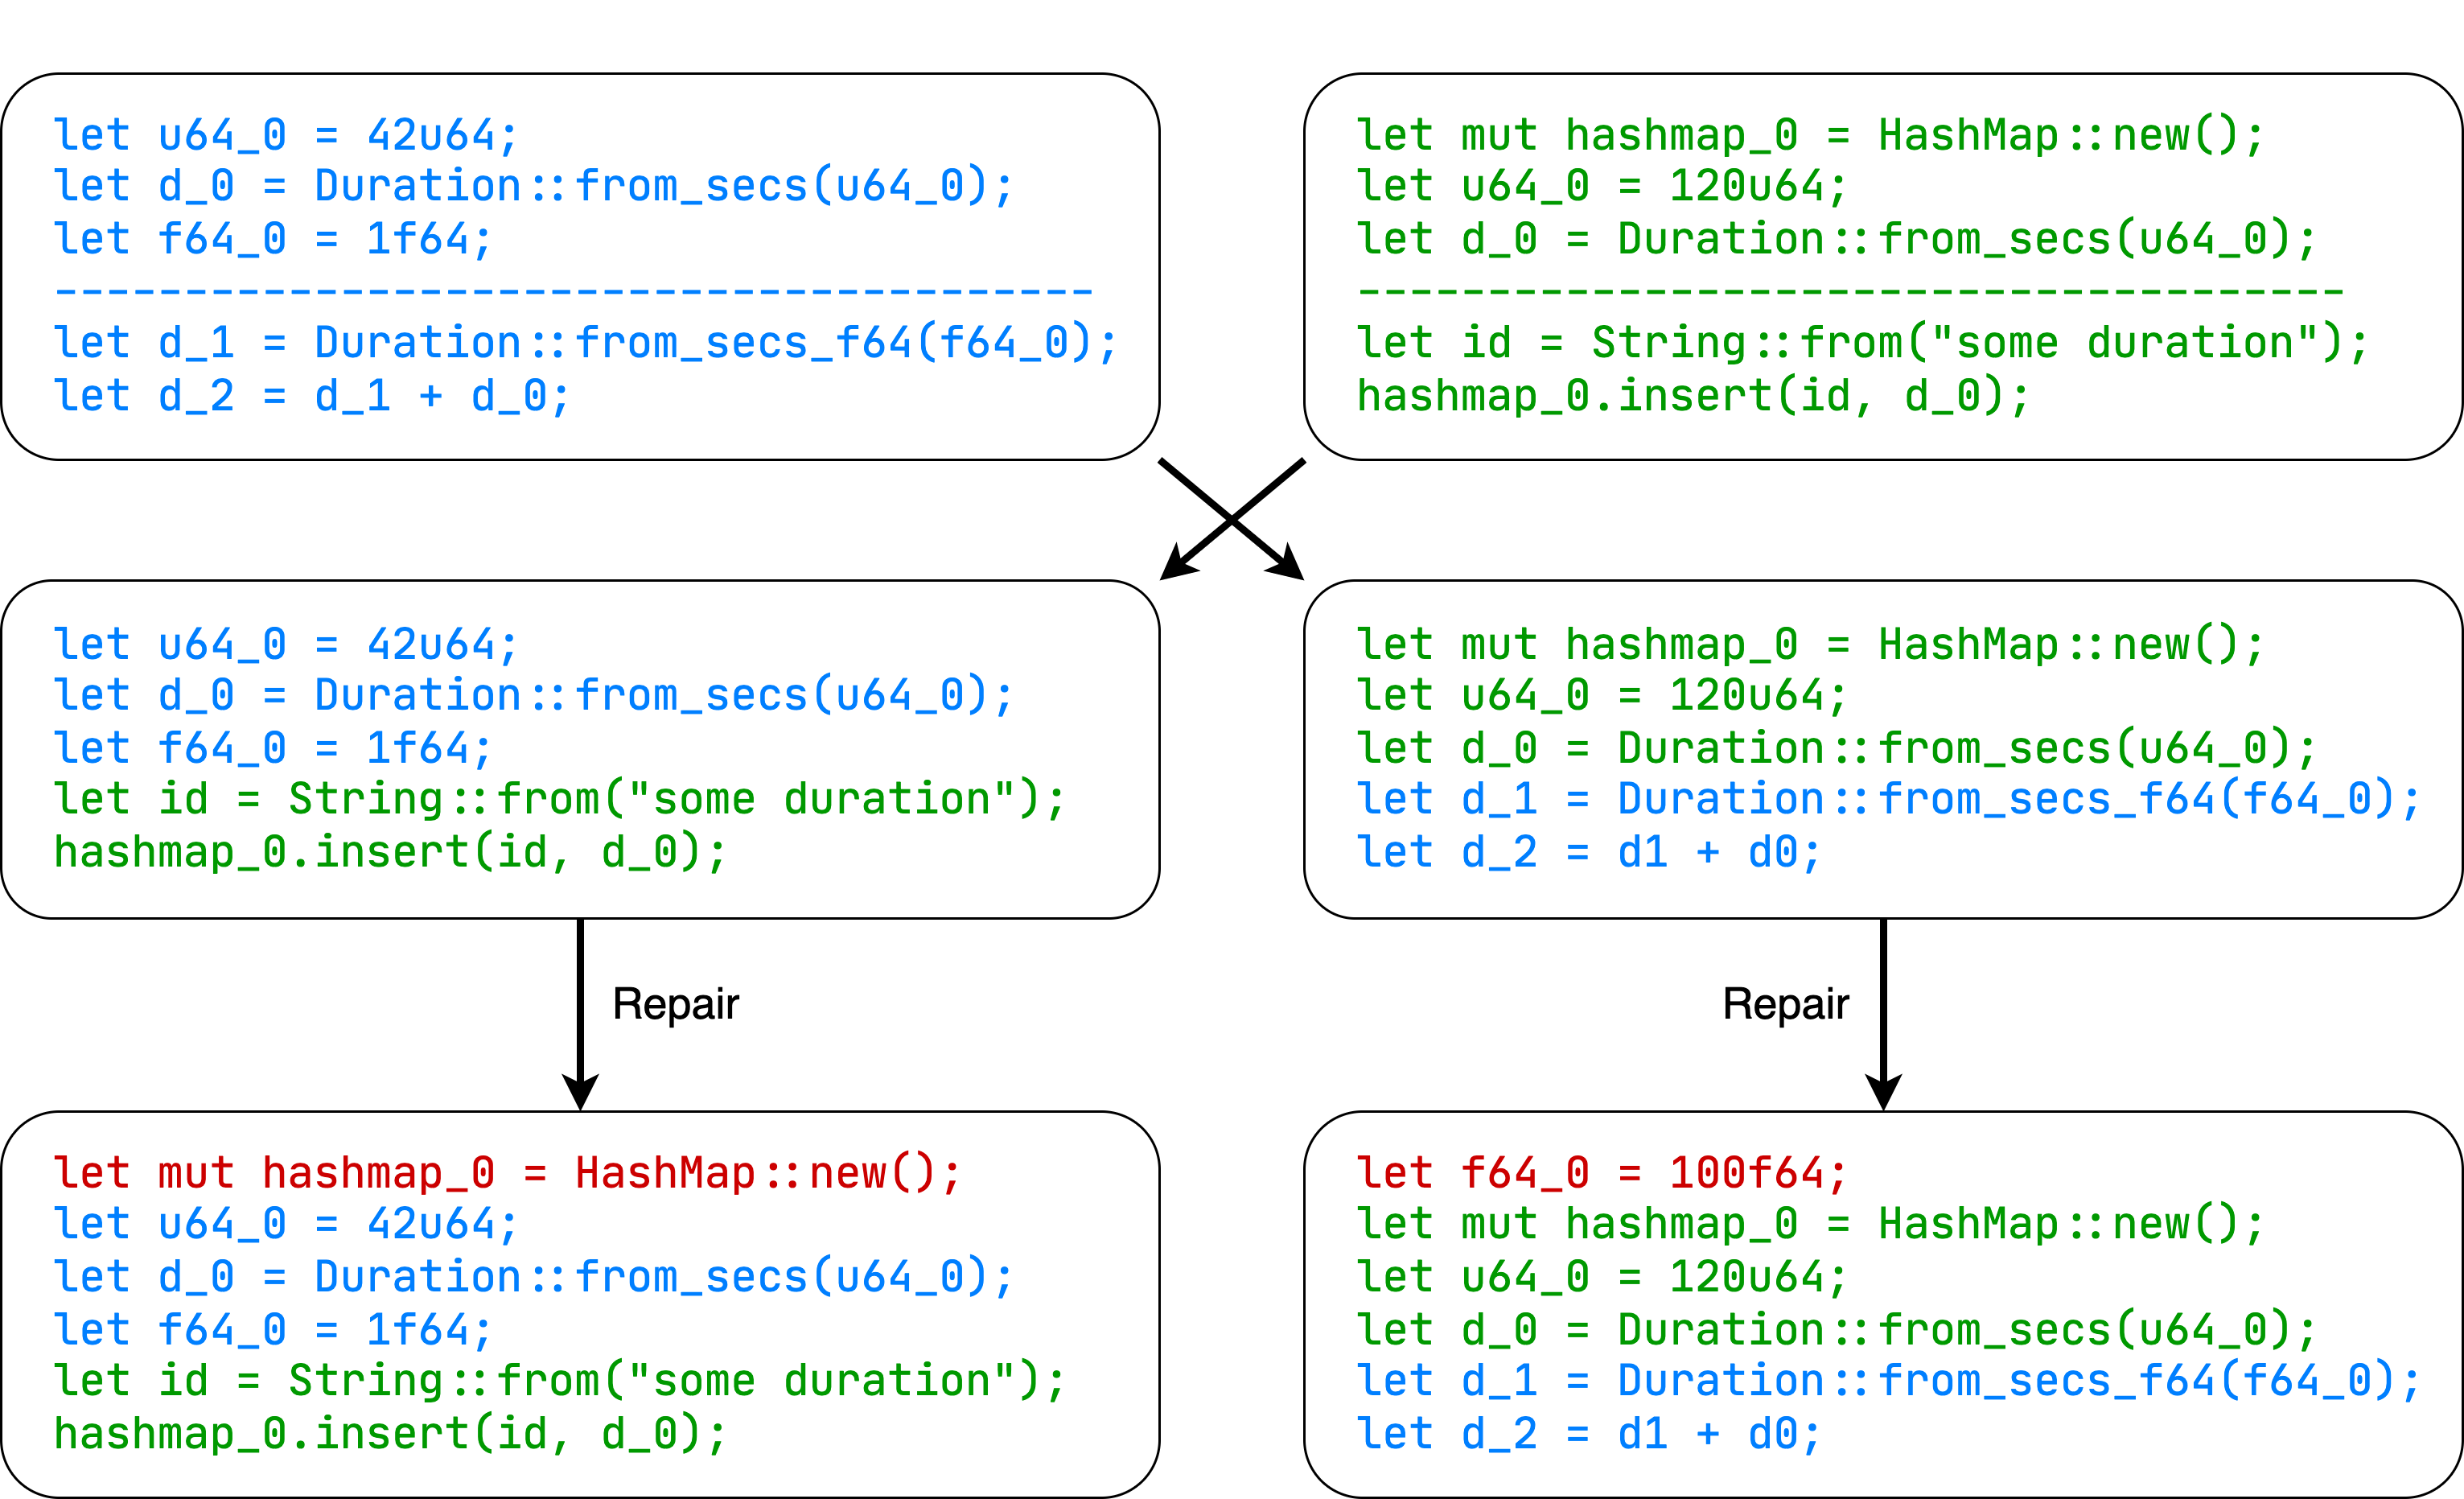
\includegraphics[width=\textwidth]{crossover}
\label{fig:crossover-example}
\end{figure}

However, recombination can also make some variables redundant, such as \texttt{hashmap\string_0} in the right recombined test case. It is no longer necessary for the test, makes it more confusing and does not increase coverage. Such cases can theoretically be filtered out using techniques such as delta debugging, however we leave them for now as they do no harm.

\subsection{Dependencies}
Assume a Rust program like in \Cref{lst:example-rust-program}, which consists of a struct type for rectangles and a struct which performs operations on the rectangle.
\begin{lstlisting}[style=boxed, caption={Rectangle data type}, label=lst:example-rust-program]
struct Rectangle {
    width: u64,
    height: u64,
}

impl Rectangle {
    pub fn new(width: u64, height: u64) -> Self {
        Rectangle { width, height }
    }
    pub fn width(&self) -> u64 {
        self.width
    }
}

struct Calculator {}

impl Calculator {
    pub fn new() -> Self {
        Calculator {}
    }
    pub fn area_by_value(&self, r: Rectangle) -> f64 {
        r.height as f64 * r.width as f64
    }
}
\end{lstlisting}

An example test case for the program can look like in \Cref{lst:example-testcase}. Here, a rectangle of a given length and width is created and consumed by the Calculator to determine the area of the rectangle. The affine type system of Rust does not allow the variable~\texttt{calculator\string_0} to be used again. Thus, after the statement in line 4, the attributes of the rectangle cannot be accessed, nor can the rectangle serve as an argument for further calls.

\begin{lstlisting}[style=boxed, caption={An example test case generated for the program in \Cref{lst:example-rust-program}}, label=lst:example-testcase]
let mut rectangle_0 = Rectangle::new(205u8, 166u8);
let u64_0 = rectangle_3.width();
let mut calculator_0 = Calculator::new();
let f64_4 = areacalculator_0.area_by_value(rectangle_0);
\end{lstlisting}


\subsection{Fitness Function}
% Um die Selektion von Parents für die nachkommende Generationen besser guiden zu können, werden alle Individuen in einer Population nach ihrer Fitness ausgewertet. Eine gute Fitnessfunktion ist sehr wichtig bei der Suche nach Lösungen. Lösungen, die in einer bestimmten Weise ''besser'' als andere sind, sollen mit besseren Fitnesswerten belohnt werden. Was auch immer eine bessere Fitness ist, eine höhere oder niedrigere Fitness hängt davon ab, ob die Suchstrategie versucht, die Fitnessfunktion zu maximieren oder zu minimieren~\cite{McMinn_2004}.

In order to better guide the selection of parents for future generations, all individuals in a population are evaluated according to their fitness. A good fitness function is very important in the search for solutions. Solutions that are ''better'' than others in a certain way should be rewarded with better fitness values. Whatever is a better fitness, a higher or lower fitness depends on whether the search strategy tries to maximize or minimize the fitness function~\cite{McMinn_2004}.

% Bei der Suche verwenden wir die Branch Coverage, d. h., jeder Branch ist ein Target. Wenn ein Branch ausgeführt wird, wird der entsprechende Test in Bezug auf diesen Target als gut markiert. Wird eine Funktion oder Methode ausgeführt, ein Branch jedoch nicht, dann bestimmt die Fitness die Distanz des jeweiligen Test Cases zur einer Ausführung des Targets. Wir verwenden die weit verbreitete Definition der Fitness für Branch Coverage, \textit{approach level} und \textit{branch distance} Berechnung, die in der such-basierten Generierung der Test Daten eingesetzt wird~\cite{McMinn_2004}. Der Approach Level beschreibt wie weit ein Test Case von einem Target im \ac{CFG} entfernt war, wenn der Test Case vom Kurs abgewichen ist. Wir berechnen den Approach Level in der Anzahl der verfehlten Control Dependencies zwischen dem Target und dem Punkt, an dem der Test Case eine falsche Abzweigung genommen hat. Approach Level ist gleich 0 wenn alle kontrollabhängige Branches vom Test Case erreicht wurden.


In the search, we use branch coverage, i.e., each branch is a target. When a branch is executed, the corresponding test is marked as good with respect to this target. If a function or method is executed but a branch is not, then the fitness determines the distance of the respective test case to an execution of the target. We use the widely used definition of fitness for branch coverage, \textit{approach level} and \textit{branch distance} computation, which is used in search-based generation of test data~\cite{McMinn_2004}. The approach level describes how far a test case was from a target in the \ac{CFG} when the test case deviated from the course. We compute approach level in terms of the number of missed control dependencies between the target and the point where the test case took a wrong turn. Approach level is equal to $0$ if all control dependency edges were reached by the test case.

% TODO reword
The branch distance estimates how far the branch at which execution diverged is from evaluating to the necessary outcome. To determine these values, the test case has to be executed once on the unmodified software. If the target executed, then approach level and branch distance are $0$. Otherwise, the rules from \Cref{tab:local-branch-distance-formulas} are used for calculation of numeric values. For all other cases, the local branch distance is either $0$ or $1$ depending on whether the respective branch was executed or not. Assume the function \texttt{bar} from \Cref{lst:example-branch-distance-boolean-flag} which takes a boolean named \texttt{flag}. When called \texttt{bar(true)}, the branch distance for the \textit{true} branch is $0$ since it gets executed, while the branch distance for the \textit{false} branch is $1$ because we do not know how the boolean value has been computed. It could be a result of some numbers comparison, a function call, or just a constant. Figuring that out requires complex static analysis that is not in the scope of \textsc{RustyUnit}. 

\begin{lstlisting}[style=boxed, caption={Computation of local branch distance for a boolean flag that we do not know where it came from}, label=lst:example-branch-distance-boolean-flag]
fn bar(flag: bool) {
    if flag {
      println!("Flag is true"); 
    } else {
      // ...
    }
}
\end{lstlisting}

Of course, not every program uses only comparisons of numbers and thus many values for the branch distance will be binary. This means that the approach level has a much more important meaning for the search. Consider the following example function \texttt{foo}:

\begin{lstlisting}[style=boxed, caption=, label=lst:example-branch-distance-nesting]
fn foo(x: i32, y: i32) -> i32 {
    if x < 5 {
        if y >= 10 {
            0
        } else {
            1
        }
    } else {
        2
    }
}
\end{lstlisting}

Assume that a test invokes \texttt{foo}. In \Cref{tab:example-fitness-calculation}, calls to \texttt{foo} with various arguments and the resulting approach level (AL) and branch distance (BD) are shown as examples .
\begin{table}[h!]
\centering
\begin{tabular}{c|cc|cc|cc}
\hline
& \multicolumn{2}{c|}{\textbf{foo(0, 5)}}                     & \multicolumn{2}{c|}{\textbf{foo(6, 1)}}                      & \multicolumn{2}{c}{\textbf{foo(0, 10)}}                     \\
\cline{2-7}
\textbf{Branch (Line)} & AL & BD & AL & BD & AL & BD \\
\hline
3-7                    & 0                       & 0                        & 0                       & 2                        & 0                       & 0                        \\
9                      & 0                       & 5                        & 0                       & 0                        & 0                       & 5                        \\
4                      & 0                       & 5                        & 1                       & 2                        & 0                       & 0                        \\
6                      & 0                       & 0                        & 1                       & 2                        & 0                       & 1 \\ \hline
\end{tabular}
\caption{Fitness value calculation for different invocations of \texttt{foo}}
\label{tab:example-fitness-calculation}
\end{table}

% TODO reword
As usual in the \ac{SBST} literature, the branch distance should not dominate the approach level, and therefore it is normalized in the range $[0, 1]$, for instance, using the following normalization function initially proposed by Arcuri~\cite{Arcuri_2011}:

\[\alpha(x) = \frac{x}{x + 1}\]

This allows us to calculate the overall fitness of a test~$t$ with respect to target~$m$:
\[D_m(t) = \text{Approach Level} + \alpha(\text{Branch Distance})\]

%EvoSuite instrumentiert in der originalen Implementierung Java SUT auf Bytecode-Level und im Bytecode werden alle Loops usw. in die einfachen if-Verzweigungen überführt. Das Ziel ist es, die optimale Lösung zu finden, d. h. eine Test Suite, die möglichst hohe Branch-Coverage hat. Gleichzeitig soll es aber keine andere Testsuite geben, die bei gleicher Branch-Coverage kleiner ist bzw. kleinere Tests enthält. Einige Branches, sogenannte infeasible Branches, können evtl. gar nicht abgedeckt werden, entweder aufgrund der limitierten Repräsentation der Lösung oder weil es keine passenden Inputs existieren. Somit werden solche Tests bevorzugt bei der Evolvierung bevorzugt, die eine höhere Fitness bzgl. der Branch-Coverage haben. Bei zwei Tests mit der gleichen Coverage wird der kürzere bevorzugt.

%Um die Suche voranzutreiben, können verschiedene Heuristiken verwendet werden. \todo{Welche gibt es überhaupt?} Eine der weitverbreitesten ist Branch Distance. McMinn~\cite{McMinn_2004} beschreibt eine Sammlung von Regeln, die rekursiv angewendet werden können, um Distanz bei allen möglichen Prädikaten zu berechnen. Wenn die Ausführung des \ac{SUT} bei gegebenen Inputdaten in einem bestimmten Branch landet, so kann eine lokale Suche angewendet werden. Es wird mit Hilfe einer lokalen Fitnessfunktion abgeleitet, wie nah das Prädikat zum Auswerten zu \texttt{true} ist. Zum Beispiel, bei einem Prädikat~\texttt{x >= 10} und~\texttt{x = 5} (während der Ausführung) wird der \texttt{false} Branch getroffen. Die Distanz zum \texttt{true} Branch beträge somit~$10 - 5 + k$ mit~$k \geq 1$. Dabei wird jedes Prädikat im \ac{SUT} instrumentiert, um die Distanzen zu anderen Branches während der Ausführung des \ac{SUT} zu tracen. Die Branch-Distanz muss noch normalisiert werden (je nach Werten kann es schnell zu Extremen kommen). Arcuri~\cite{Arcuri_2011} beschreibt in seiner Arbeit, welchen Einfluss die Normalisierung der Branch-Distanz auf die Effektivität einer such-basierten Testgenerierung hat.

\begin{table}[]
\centering
\begin{tabular}{lcr}
\hline
\textbf{Condition}  & \textbf{Distance True} & \textbf{Distance False} \\
\hline
x == y              & |x - y|                & 1                       \\
x != y              & 1                      & |x - y|                 \\
x \textgreater y    & y - x + 1              & x - y                   \\
x \textgreater{}= y & y - x                  & x - y + 1               \\
x \textless y       & x - y + 1              & y - x                   \\
x \textless{}= y    & x - y                  & y - x + 1               \\ \hline
\end{tabular}
\caption{Local branch distance calculation for numeric values}
\label{tab:local-branch-distance-formulas}
\end{table}

\subsection{Test Oracles and Testability Transformations}
\label{sec:testability-transformations}


A technique called \textit{testability transformation} tries to overcome this obstacle. A testability transformation is a source-to-source program transformation that seeks to improve the performance of some chosen test data generation technique~\cite{Harman2004}, e.g., reach difficult branches. Beyond that, a \ac{SUT} can be transformed in a way such that artificial branches are inserted into the code to guide the search into triggering some exceptional behavior and crash the program. For instance, \textsc{EvoSuite}~\cite{Fraser2013} employs multiple testability transformations such as array access transformation (\Cref{lst:evosuite-array-access-transformation}), division by zero transformation, or numerical overflow transformation. Those transformations do not increase code coverage in general but contribute to discovering potential unforeseen behavior and generating inputs that trigger it.

\begin{lstlisting}[language=Java, style=boxed, caption={Array access transformation in \textsc{EvoSuite} for Java}, label=lst:evosuite-array-access-transformation]
// Original method
void foo(int x) {
    bar[x] = 0;
}

// Transformed method for better testability
void foo(int x) {
  if (x < 0) {
    throw new NegativeArraySizeException();
  }
  if (x >= bar.length) {
    throw new ArrayIndexOutOfBoundsException();
  }
  bar[x] = 0;
}
\end{lstlisting}

We apply similar ideas to \textsc{RustyUnit}. However, some of the problems that other programming languages have, do not affect Rust, e.g., there are no null pointers as in C or Java. Moreover, the Rust compiler already incorporates checks for common issues in the \ac{MIR} that are addressed by testability transformations. That is, we do not have to transform the \ac{MIR} to introduce new branches as in~\Cref{lst:evosuite-array-access-transformation}, but only trace these branches automatically inserted by the compiler. 

%\subsection{Test Minimization}
%Da sich diese Arbeit vor allem auf das Generieren vor Tests beschränkt, die möglichst hohe Coverage erreichen, jedoch generell keine Testorakel automatisch zur Verfügung stellt, sollen die Tests möglich kurz gehalten werden und das wesentliche tun, um einen bestimmten Branch zu erreichen. Das erhöht ihre Lesbarkeit und Verstänlichkeit. Fraser und Arcuri~\cite{Fraser2013a} schlagen als Verbesserung für ihr EvoSuite Tool folgendes Verfahren vor: Für jeden Coverage Goal wird ein Test aus der generierten Test Suite ausgewählt, der diesen Goal abdeckt. Dieser Test wird wrt to the coverage goal minimiert, so dass Statements, die nicht zur Ausführung des Goals beitragen, gelöscht werden. Wenn ein Goal bereits von einem minimierten Test abgedeckt ist, so wird kein weiterer Test für diesen Goal der finalen Test Suite hinzugefügt. Auf diese Weise werden Tests lesbarer für einen Menschen und können somit leichter manuell um Testorakel ergänzt werden.

%Since this work is mainly limited to generating tests that achieve the highest possible coverage but do not provide test oracles automatically in general, the tests should be kept as short as possible and do the essential to achieve a certain branch. This increases their readability and comprehensibility. Fraser and Arcuri~\cite{Fraser2013a} propose the following procedure as an improvement for their EvoSuite tool: for each coverage goal, a test is selected from the generated test suite that covers that goal. That test is minimized with respect to the coverage goal so that statements that do not contribute to the execution of the target are removed from the test. If a target is already covered by a minimized test, no further test for this objective will be added to the final test suite. This way, tests become more readable to a human and can thus be more easily supplemented manually with test oracles.

\clearpage
\chapter{Implementation}
\label{chap:implementation}
In this chapter we present essential parts of the implementation of \textsc{RustyUnit}. To generate tests, \textsc{RustyUnit} needs access to the source code of the \ac{SUT} since, unlike \textsc{EvoSuite} for Java, for isntance, the required analysis and instrumentation does not take place on the compiled binary, but during the compilation process itself. The Rust compiler provides a convenient interface for controlling the compilation process. We register the analysis of the target program and instrument it using this interface. Die Ergebnisse der Analyse werden für die Generierung und Synthesis der Tests benötigt, während die Instrumentierung nötig ist, um die generierten Tests bei deren Ausführung auf ihre Fitness zu bewerten. Am Ende der Suche entsteht eine finale Testsuite in Form von Rust Quellcode zur Verfügung.

% Die Übesicht des ganzen Prozesses
\begin{figure}[h!]
\caption{High-level overview of the steps to generate tests from a crate}
\centering
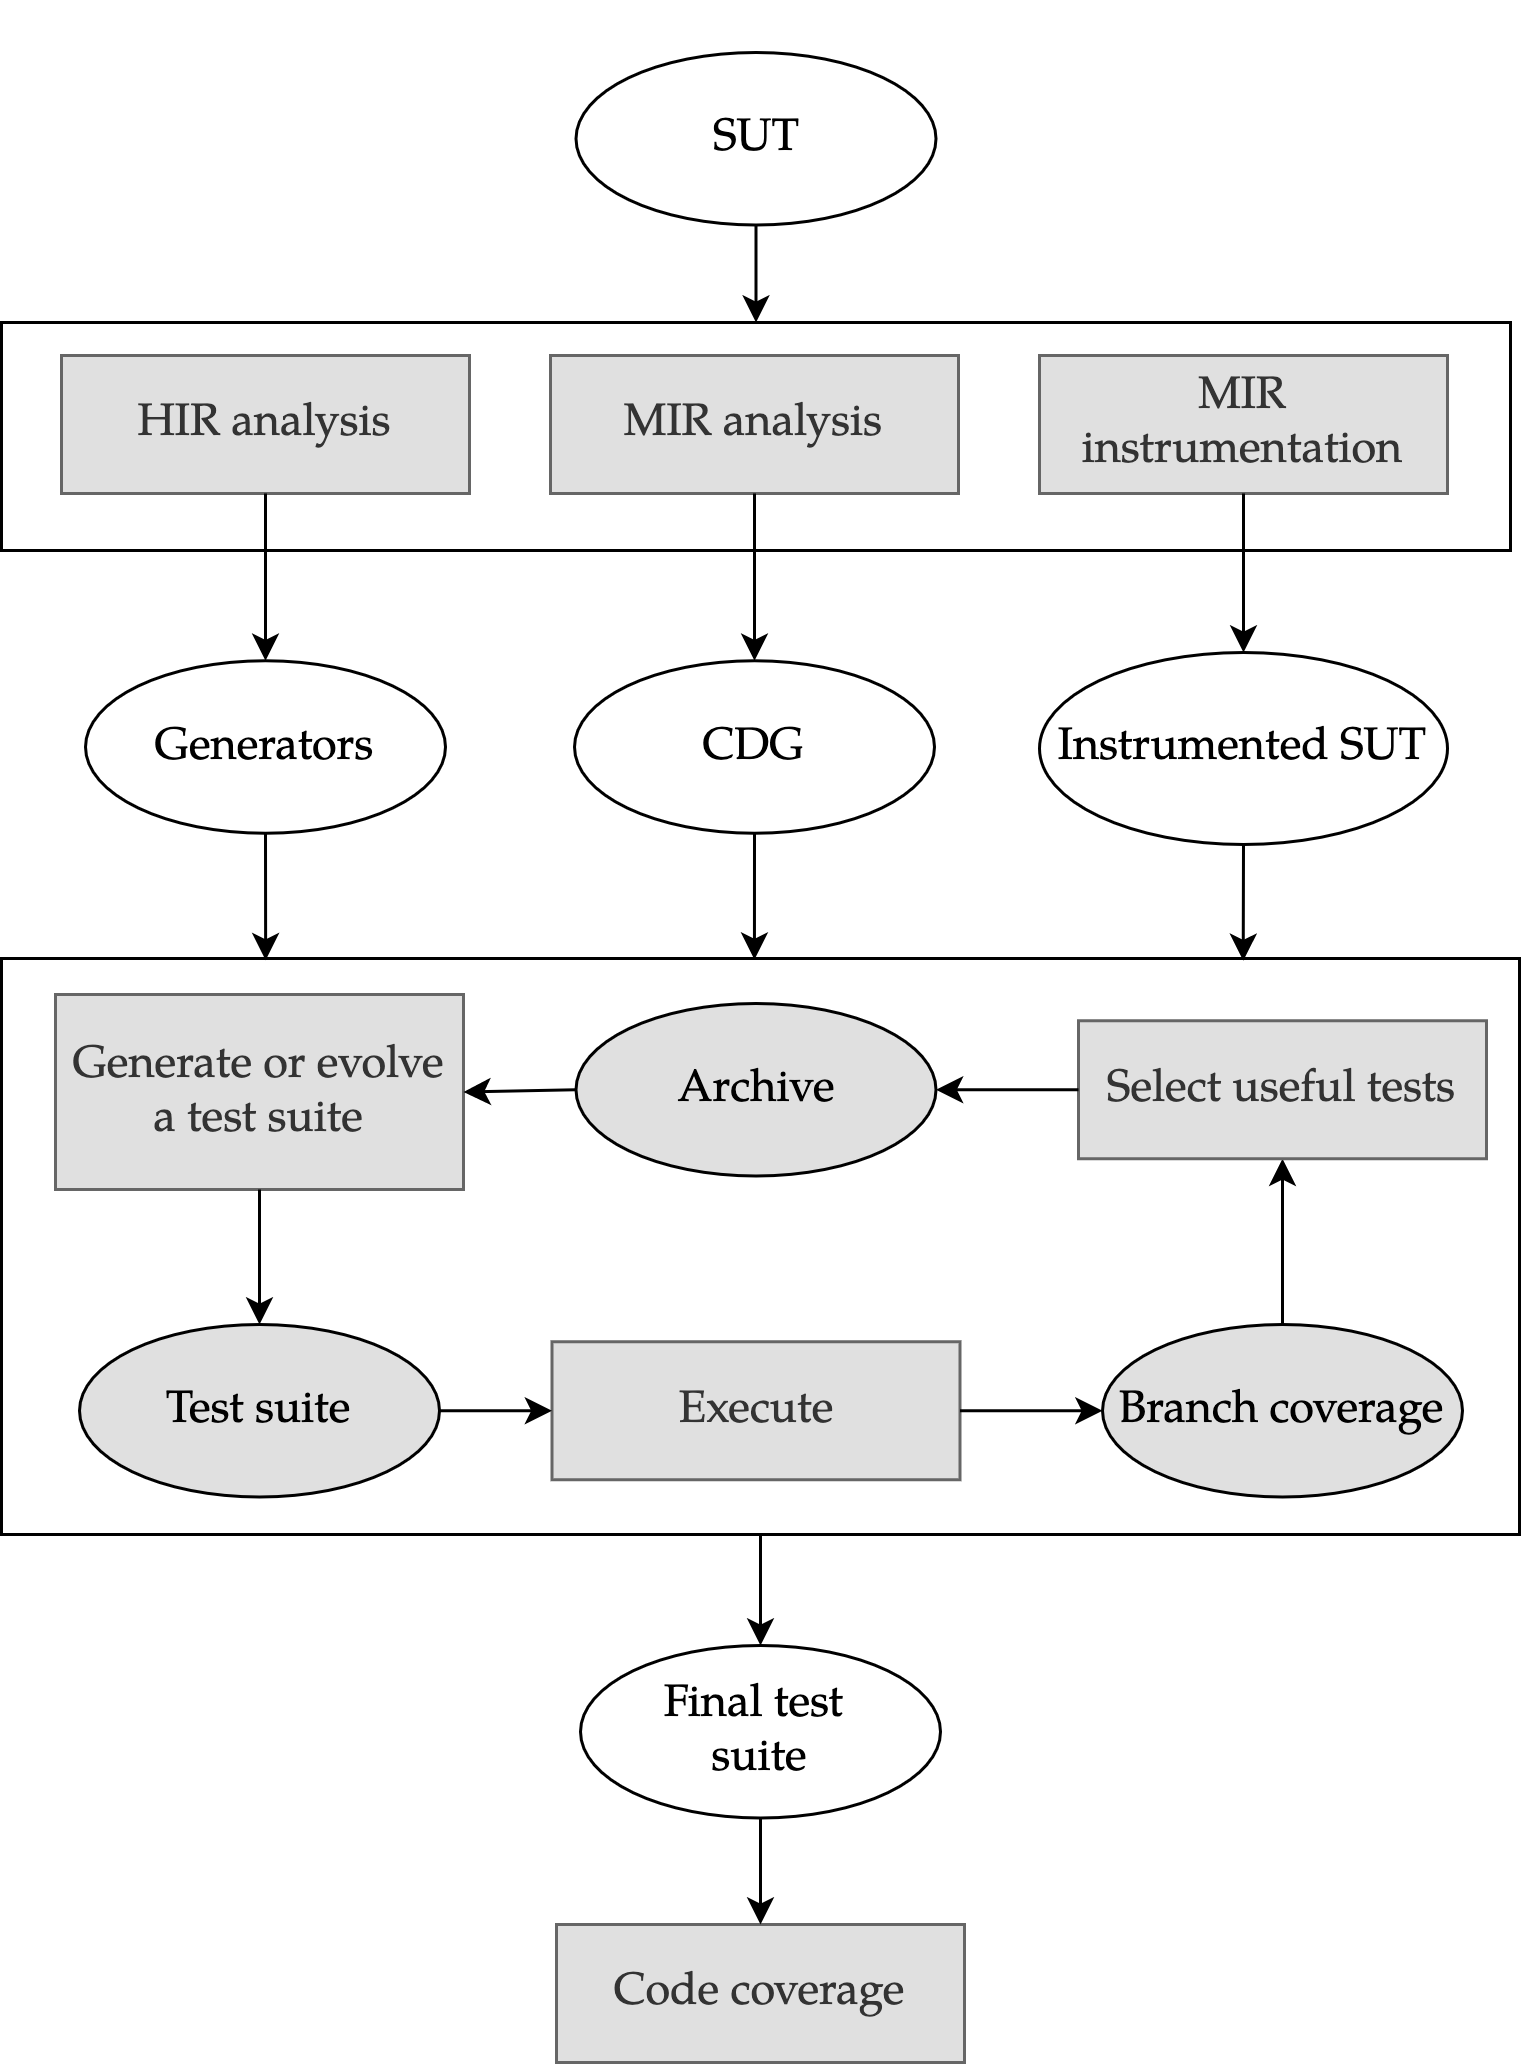
\includegraphics[width=\textwidth]{overview}
\label{fig:rustyunit-overview}
\end{figure}

\section{Using the Compiler Hooks}
The Rust compiler design makes it possible to use it both, as an executable and as a collection of libraries. To this end, Rust provides compiler crates, which can be recognized by their common prefix, \texttt{rustc}, such as \texttt{rustc\string_driver}, which is an interface for running the compiler programmatically.

To have access to the compiler internals, multiple things are required. Firstly, the internals are unstable and probably will never be. As such, programs that use compiler internals must do using \textit{nightly} versions of Rust. Secondly, the crates must have the \texttt{rustc\string_private} feature enabled, which allows crates to access individual compiler crates. Thirdly, these crates must be explicitly specified in the crate root using the \texttt{extern crate} keywords. For instance, if the program needs the internal \texttt{rustc\string_driver}, it must specify it the following way in the crate root: \texttt{extern crate rustc\string_driver;}

With compiler internals available, we can implement some of the callbacks that the compiler will call at appropriate time. The \texttt{rustc\string_driver::Callbacks} trait defines four callbacks, which are called in the following order:
\begin{enumerate}
    \item \texttt{config}
    \item \texttt{after\string_parsing}
    \item \texttt{after\string_expansion}
    \item \texttt{after\string_analysis}
\end{enumerate}

The \texttt{config} method will be called before creating the compiler instance and allows to change the default compiler configuration. Each of the other three functions will be called after the end of the corresponding compilation phase. The interface provides the \texttt{after\string_*} hooks with an instance of the compiler and, more important, with a \texttt{Queries} object which allows to query the global context of the program under compilation and also the \ac{HIR} and \ac{MIR}. It is very convenient because this way we can extract all the items defined in the target crate, including functions and methods along with their parameters and return types. We need this data to know what statements can be placed in a generated test. Another important point is that at this stage we can obtain full type paths, which the compiler has resolved until then, e.g., \texttt{std::fs::File} instead of just \texttt{File}.

\begin{lstlisting}[style=boxed, caption={The Rust compiler interface accepts an object which implements its callback trait, allowing us to execute code at different compilation phases}, label=lst:compiler-callbacks]
struct CompilerCallbacks;

type mir_fn_ptr = for<'tcx>
  fn(_: TyCtxt<'tcx>, _: DefId) -> &'tcx Body<'tcx>;

impl rustc_driver::Callbacks for CompilerCallbacks {
  fn config(&mut self, _config: &mut Config) {
    _config.override_queries = Some(|_, _, external| {
      let fn_ptr: mir_fn_ptr = |tcx, def_id| {
        let opt_mir
          = rustc_interface
            ::DEFAULT_EXTERN_QUERY_PROVIDERS
            .borrow().optimized_mir;
        let mut body = opt_mir(tcx, def_id).clone();
        let crate_name = tcx.crate_name(def.krate);
        let hir_id = tcx.hir()
          .local_def_id_to_hir_id(def.expect_local());

        if is_extern(crate_name)
            || is_our_monitor(hir_id, &tcx) {
          // Do not instrument extern crates
          // or our own instrumentation code
          return tcx.arena.alloc(body);
        }

        let mut mir_visitor = MirVisitor { tcx };
        mir_visitor.visit_body(&mut body);
        tcx.arena.alloc(body)
      };
      external.optimized_mir = fn_ptr;
    });
  }
}
\end{lstlisting}
However, even though a \ac{MIR} object is clonable and can be modified, there is no way to pass a modified version back to the compiler within a callback because both parameters are immutable. The compiler performs several distinct optimizations on the \ac{MIR}, called passes. Accordingly, they can modify the \ac{MIR}. In the earlier compiler versions it was possible to register a custom MirPass~\footnote{\url{https://doc.rust-lang.org/stable/nightly-rustc/rustc_mir/transform/trait.MirPass.html}} as part of a compiler plugin, but this possibility was later eliminated. However, there is still a way that allows us to propagate changes to the \ac{MIR} back to the compiler, instead of extending it and building an own version of it. The \texttt{config} callback provides a mutable \texttt{Config} object which allows to replace the default \ac{MIR}-providing function \texttt{optimized\string_mir} (among many others) with an own custom implementation. As shown in \Cref{lst:compiler-callbacks}, a provider for an optimized \ac{MIR} is a function pointer. Our custom provider implementation is a basic wrapper, which first obtains the original \ac{MIR} object using the default implementation, applies the \texttt{MirVisitor}, which mutates the \ac{MIR} in-place, and returns the mutated version. The compiler invokes the \texttt{optimized\string_mir()} Provider in further steps, and thus, the mutated \ac{MIR} object will be propagated.

\begin{lstlisting}[style=boxed, caption={Running the Rust compiler like a library}, label=lst:running-compiler]
fn run_rustc() -> Result<(), i32> {
  let std_env_args: Vec<String> = std::env::args()
    .collect();
  let rustc_args = get_compiler_args(&std_env_args);
  pass_to_rustc(&rustc_args);
  return Ok(());
}

pub fn pass_to_rustc(rustc_args: &[String]) {
  let mut callbacks = MirCallbacks {};

  let err = rustc_driver::RunCompiler::new(
    &rustc_args, &mut callbacks
  ).run();
  if err.is_err() {
    eprintln!("Error while compiling dependency");
    std::process::exit(-1);
  }
}

fn main() {
  exit(
    run_rustc()
      .err()
      .unwrap_or(0),
  )

}
\end{lstlisting}

\Cref{lst:running-compiler} shows how the Rust compiler can subsequently be started programmatically. Now this program can be used in general for instrumenting Rust programs. However, calling it directly is very cumbersome, since the compiler needs to know many arguments, especially for large crates, in order to link dependencies correctly. Normally one uses a build system for this, for example Cargo, which takes over this work and provides appropriate compiler arguments when building a crate. Fortunately, Cargo provides a way to define our own \texttt{rustc} wrapper, which is then supplied with correct CLI arguments by Cargo. The task of such a wrapper is to eventually call the compiler on itself with the passed arguments~\footnote{\url{https://doc.rust-lang.org/cargo/reference/environment-variables.html}}. To use the wrapper, one has to set the environment variable \texttt{RUSTC\string_WRAPPER} to the path to the wrapper binary. Finally, a target Rust program can be built and instrumented by running:

\texttt{RUSTC\string_WRAPPER=./instrumentation cargo \string+nightly build}

Since our wrapper uses \texttt{rustc\string_private} features, we have to tell Cargo to enable the nightly channel. The next step is to define how to instrument the \ac{MIR} so that we can observe the execution paths triggered by an execution of generated tests.

%The whole process starts, when we run the compiler for the first time on a target crate that we want to test. During this process we can already extract the available items like structs and their methods by traversing the \ac{HIR}.

\section{HIR Analysis}
For the purpose of test generation, \ac{HIR} and \ac{MIR} are of primary importance. First, we are interested in all possible functions, structs/enums, and their methods and fields in the crate we want to test. This information allows us to evaluate which statements we can use in a generated test at all and what types of instances do those statements produce. We call functions and methods generators since those can generate instances and values of the required types when we recursively search for a dependency. The fact that desugaring has already been performed in the \ac{HIR} has no influence at this point, because the transformations are only performed intra-procedurally. We are only interested in type and method definitions, their parameters and return types, which still remain unchanged at this level. Moreover, thanks to \ac{HIR} we can also determine the absolute path of a type, for example a parameter. Relative type names, such as \texttt{File} instead of \texttt{std::fs::File}, can lead to difficulties when compiling the generated tests due to missing imports. Thus, it is easier to carry a complete type path, and by means of \ac{HIR} we can easily query this.

% TODO reword
The top-level data structure in the \ac{HIR} is the \texttt{Crate}, which stores the contents of the crate currently being compiled. The Rust compiler compiles crates independently and, thus, only ever constructs \ac{HIR} for the current crate. Technically, the \ac{HIR} \texttt{Crate} structure contains a number of maps that serve to organize the content of the crate for easier access. For instance, the contents of individual items (e.g., modules, functions, traits, impls and so on) in the \ac{HIR} are not directly accessible in the parents. So, for example, if there is a module item \texttt{foo} containing a function \texttt{bar()}:

\begin{lstlisting}[style=boxed, caption={}]
mod foo() {
    fn bar() { }
}
\end{lstlisting}
then in the \ac{HIR}, the representation of module \texttt{foo} would only have the ID \texttt{I} of \texttt{bar()}. To get the details of the function, we would lookup \texttt{I} in the \texttt{items} map of the \ac{HIR}, as shown in \Cref{lst:hir-analysis}. One nice result from this representation is that one can iterate over all items in the crate by iterating over the key-value pairs in these maps (without the need to trawl through the whole \ac{HIR}). The other reason for such decoupled design is for better integration with incremental compilation. This way, if we gain access to some item, e.g., for the module \texttt{foo}, we only gain access to the id for \texttt{bar()}, and we must invoke some functions to lookup the contents of the function given its id. This gives the compiler a chance to observe that we accessed the data for \texttt{bar()}, and then record the compilation dependency.

In \Cref{lst:hir-analysis} we iterate over the \texttt{items} map of the \ac{HIR} and extract the relevant elements like functions, structs, and methods by pattern matching the type of an item. Each item stores a \texttt{Span} object, which shows its origin at the source code level, i.e., the source file it has been defined within. This is important for us because in Rust, unlike, for instance, in Java, unit tests can and should, by convention, be written into the files that contain the code to test. This also means that unit tests, also our generated tests, can invoke private functions and methods directly, which in turn can lead to higher coverage.

% TODO also add enums and traits
\begin{lstlisting}[style=boxed, caption={Iterate over the items in the HIR of a crate}, label=lst:hir-analysis]
fn hir_analysis(
  tcx: &TyCtxt<'_>, callables: &mut Vec<Callable>
) {
  for item in tcx.hir().items() {
    match &item.kind {
      ItemKind::Fn(sig, _, _) => {
        if &item.ident.name.to_string() != "main" {
          analyze_fn(sig, item.def_id,
            &mut callables, &tcx);
        }
      }
      ItemKind::Impl(impl_item) => {
        if allowed_item(item, &tcx) {
          analyze_impl(impl_item, &mut callables, &tcx);
        }
      }
      ItemKind::Struct(s, g) => {
        if allowed_item(item, &tcx) {
          analyze_struct(item.def_id, s, g, &item.vis,
          file_path.unwrap(), &mut callables, &tcx);
        }
      }
      _ => {
        // Ignore the other items
      }
    }
  }
}
\end{lstlisting}

This way we can already generate random tests, since we know which functions or methods can be called. \Cref{lst:hir-analysis-example} shows an example program. After the analysis, the following holds in terms of \Cref{alg:genobject}: $M = \{\texttt{Address::new}, \texttt{Person::new}, \texttt{Person::address}, \texttt{say\string_hello\string_to}, \texttt{address\string_to\string_string}\}$. If we wanted to execute the \texttt{address\string_to\string_string} function in an empty test $t = \{\}$, we would have to generate an argument of type \texttt{Address}. Thanks to the information about the return type of a method, we can use $GenObject(Address, \{\}, M, t)$ to create either an \texttt{Address} object using \texttt{Address::new} or \texttt{Person::address}. The latter one is a method, i.e., it expects a \texttt{self} object argument which would require us to recursively search for a way to create an object of type \texttt{Person}, e.g., by calling the constructor \texttt{Person::new}.

\begin{lstlisting}[style=boxed, caption={After HIR analysis, we know how a \texttt{Person} object can be generated to be used in \texttt{say\string_hello\string_to}.}, label=lst:hir-analysis-example]
struct Address {
  street: String,
  house_n: usize,
  city: String,
  zip: usize
}

impl Address {
  pub fn new(street: &str, house_n: usize,
  city: &str, zip: usize) -> Self {
    Address {
      street: street.to_owned(),
      house_n,
      city: city.to_owned(),
      zip
    }
  }
}

struct Person {
  name: String,
  address: Address
}

impl Person {
  pub fn new(name: &str, address: Address) -> Self {
    Person {
      name: name.to_owned(),
      address
    }
  }

  pub fn address(&self) -> &Address {
    &self.address
  }
}

fn say_hello_to(person: &Person) {
  // ...
}

fn address_to_string(address: &Address) -> String {
  // ...
}
\end{lstlisting}

\section{MIR Analysis}
Hier muss die Analyse der MIR beschrieben werden, also wie wird die MIR (CFG) zum Post-Dominator Tree und dann zum CDG umgewandelt. Einige der Nodes sind bereits Objectives, die gecovert werden müssen.

% Building CDG from MIR
To improve the effectivity of generated tests, both DynaMOSA and the used fitness function (approach level) rely on information from a \ac{CDG}~\cite{Ferrante1987} of the \ac{SUT}. A \ac{CDG} can be constructed from a \ac{CFG} and its post-dominator tree. \ac{MIR} itself is a \ac{CFG}, so before instrumenting it, we can build the post-dominator-tree and the \ac{CDG} of each method we want to test. We do not use the complete \ac{CFG} of a \texttt{Body}, but rather a subset of it. Rust compiler creates many unwinding edges that point to basic blocks whose task is to cleanup the stack in case the program panics at some points of it's execution. However, here we only want to analyse and test regular program execution, not the cleanup logic of the compiler. Furthermore, considering unwind nodes results in \ac{CFG} having multiple exit nodes, which complicate the computation of a post-dominator tree. The standard algorithm to compute a dominator tree from a \ac{CFG} can also yield a post-dominator tree when applied to reversed \ac{CFG}, given that the original \ac{CFG} has a single exit point, i.e., a single entry point with reversed edges.

Prosser introduced the notion of dominance in a 1959 paper on the analysis of flow diagrams, defining it as follows:
\textit{We say box i dominates box j if every path (leading from input to output through the diagram) which passes through box j must also pass through box i. Thus box i dominates box j if box j is subordinate to box i in the program}~\cite{Prosser1959}. He did not specify the algorithm to compute dominance, though. Since then, several algorithms for calculating dominance have been presented. Post-dominance can be computed the same way on a \ac{CFG} with reversed edges, given that the \ac{CFG} has a single exit point. In this work, we use the \texttt{petgraph} graph library for Rust, which provides an implementation of the simple, fast dominance algorithm~\cite{Cooper2001} by Cooper et al. Finally, we compute a \ac{CDG} for each method body based on the algorithm~\cite{Ferrante1987} described by Ferrante et al.

\section{MIR Instrumentation}
The only compiler callback we implement at is point is the \texttt{config} function, which allows us to modify the \ac{MIR} of a target program on the fly. The internal compiler crates already provide a \texttt{MutVisitor}~\footnote{\url{https://doc.rust-lang.org/nightly/nightly-rustc/rustc_middle/mir/visit/trait.MutVisitor.html}} which can be used to traverse and modify \ac{MIR} objects. To trace the execution of branches of a \ac{SUT}, we need to insert additional code at relevant places in the \ac{MIR}. Those are mainly entry basic blocks (to trace if a body has been entered at all during an execution of a test) and basic blocks that introduce branches and split the execution flow, e.g., those having \texttt{SwitchInt} and \texttt{Assert} terminators. Technically, there are also other terminators which have more than one successor, e.g., \texttt{Call}s, which are function invocations. However, the optional additional branch is used to point to basic blocks which unwind the stack in case the function being called panics, i.e., the program crashes. At this point, we are only interested in basic blocks that belong to the regular execution of the program. \Cref{lst:example-function-to-instrument,lst:mir-of-example-function-to-instrument} show an example function we want to instrument and the relevant parts of it's \ac{MIR}.

\begin{lstlisting}[style=boxed, caption={Example function to instrument}, label=lst:example-function-to-instrument]
fn foo(x: i32, y: i32) {
  if x < y {
    println!("x < y");
  } else {
    println!("x >= y");
  }
}
\end{lstlisting}

Within the entry basic block in the \ac{MIR}, the two input arguments are compared and their result is stored into the local variable~\texttt{\string_3}. Then, based on the comparison result, the execution of the function can either jump to the block~\texttt{bb1} (if~\texttt{x} was less than~\texttt{y}) or \texttt{bb3} (if~\texttt{x} was greater or equal to~\texttt{y}), that is, there are two branches at this point.
\begin{lstlisting}[style=boxed, caption={MIR of the \texttt{foo} function}, label=lst:mir-of-example-function-to-instrument]
fn foo(_1: i32, _2: i32) -> () {
  // Locals definition

  bb0: {
    _4 = _1;
    _5 = _2;
    _3 = Lt(move _4, move _5);
    switchInt(move _3) -> [
      false: bb2, otherwise: bb1
    ];
  }

  bb2: {
    // print "x >= y"
  }

  bb1: {
    // print "x < y"
  }

  // Other blocks
}
\end{lstlisting}

For simplicity, we will consider individual instrumentation methods separately in the next chapters. Effectively, however, they will all be used together to trace various aspects of program execution.

\subsection{Body Entry Instrumentation}
To trace the entry of a function, we have to insert a call to our monitor at the very beginning. A function call is always a terminator in \ac{MIR}; that is, we must insert a whole new basic block for each trace function invocation. It must be the very first block in the sequence of basic blocks of the respective function, i.e., \texttt{bb0}, so we shift the original blocks by one and let our new artificial tracing block point to the original entry block, which is \texttt{bb1} now. Since the \ac{MIR} graph of each function is an independent data structure, they all have independent identificators, e.g., the id of the module and the function currently being compiled. The combination of the two allows us to uniquely identify functions. The ids are assigned by the compiler and are already known at the time of instrumentation, which is why we only weave them in as constants. Assume that the id of the module in which the function \texttt{foo} is defined is equal to $2$, and the id of the function itself is $3$. Then, after instrumenting the entry of the function, it's \ac{MIR} looks like:

\begin{lstlisting}[style=boxed, caption={}, label=lst:mir-instrument-root]
fn foo(_1: i32, _2: i32) -> () {
  // Locals definition

  bb0: {
    _3 = monitor::trace_root(
      const 2_u64, 
      const 3_u64
    ) -> bb3;
  }

  bb3: {
    _4 = _1;
    _5 = _2;
    _3 = Lt(move _4, move _5);
    switchInt(move _3) -> [false: bb2, otherwise: bb1];
  }

  bb2: {
    // print "x >= y"
  }

  bb1: {
    // print "x < y"
  }

  // Other blocks
}
\end{lstlisting}

By outsourcing calculations and the actual tracing to external \texttt{monitor::trace\string_*} functions, we need to expend minimal effort to weave in code at this low-level. The \texttt{monitor} module itself is a regular Rust source code file which we copy into the crate before compiling and instrumenting it. It is a wrapper around the branch distance and tracing logic. With this approach, \texttt{monitor} is compiled with the actual crate and is available to the instrumented code, so we can call the monitor functions directly. Assume, our \texttt{main} function looks like this:
\begin{lstlisting}[style=boxed, caption={}]
fn main() {
  foo(10, 20);
  foo(10, 20);
}
\end{lstlisting}

Then, we will get the following trace output after the instrumentation of the program:

\begin{lstlisting}[language={}, style=boxed, caption={}]
Visited root branch (2, 3)
Visited root branch (2, 3)
\end{lstlisting}

\begin{figure}[h]
\caption{Instrumented function entry}
\centering
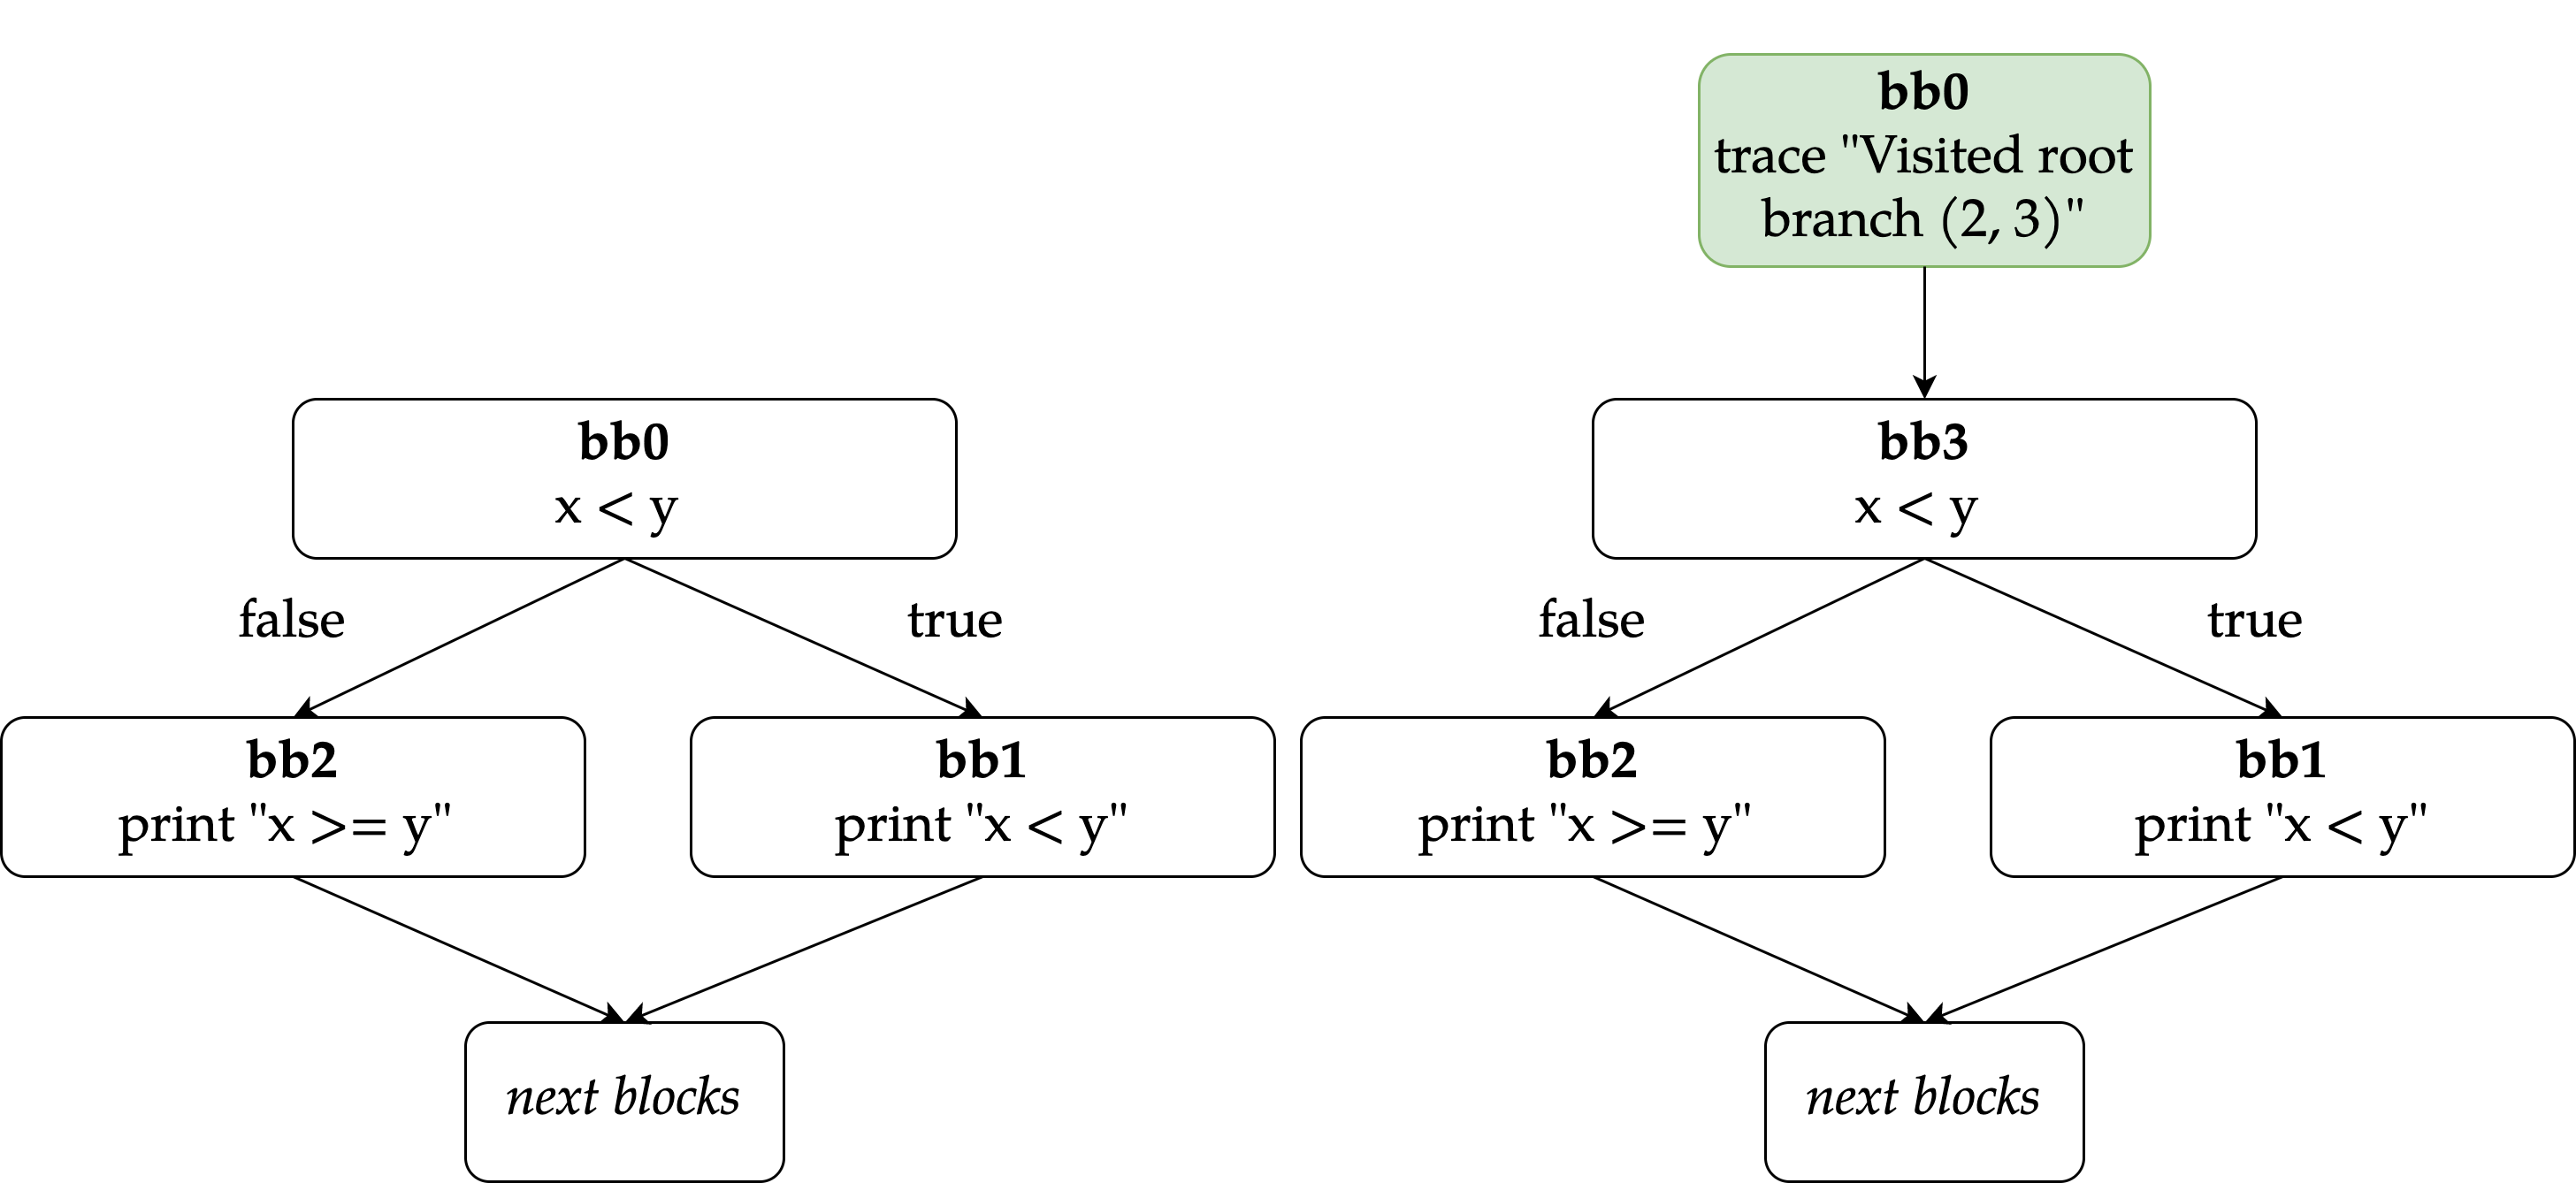
\includegraphics[width=\textwidth]{comparison-instrumented-fn-entry}
\label{fig:comparison-instrumented-fn-entry}
\end{figure}

\subsection{Branch Instrumentation}
To trace the execution of a branch, we need to insert calls to the monitor after a branch has been taken and just before it starts to execute. Doing so, we first update a terminator where branching begins, e.g., \texttt{switchInt}, to point to our artificial tracing blocks. Here, the number of tracing blocks per branch is equal to the number of branches. This is due to the fact that after a particular branch is taken, we want to trace the distance for all branches. This means that for each possible branch a call to the monitor is needed, i.e. a basic block. At this point, we know pretty much on what basis a particular branch is taken and can thus incorporate appropriate logic. Exact values are then inserted and traced at runtime. In the end, we put a chain of tracing blocks with length $l >= 2$ in each branch. Then, the last block of each tracing chain must point to the original target block of the branching terminator. \Cref{lst:mir-instrument-branch} provides an instrumented version of the \ac{MIR} shown in \Cref{lst:mir-of-example-function-to-instrument}.


\begin{lstlisting}[language={}, style=boxed, caption={Instrumented branches in the \ac{MIR} of the \texttt{foo} function}, label=lst:mir-instrument-branch]
fn foo(_1: i32, _2: i32) -> () {
  // Locals definition
  // ...
  let mut _11: monitor::BinaryOp;
  let mut _26: monitor::BinaryOp;
  let mut _34: monitor::BinaryOp;
  let mut _40: monitor::BinaryOp;


  bb0: {
    _4 = _1;
    _5 = _2;
    _3 = Lt(move _4, move _5);
    switchInt(move _3) -> [false: bb4, otherwise: bb6];
  }

  bb2: {
    // print "x >= y"
  }

  bb1: {
    // print "x < y"
  }

  bb4: {
    _8 = _1;
    _7 = move _8 as f64 (Misc);
    _10 = _2;
    _9 = move _10 as f64 (Misc);
    discriminant(_11) = 1;
    _6 = monitor::trace_branch_bool(const 2_u64,
                        const 3_u64,
                        const 2_u64,
                        move _7,
                        move _9,
                        move _11,
                        const false) -> bb5;
  }

  bb5: {
    _23 = _1;
    _22 = move _23 as f64 (Misc);
    _25 = _2;
    _24 = move _25 as f64 (Misc);
    discriminant(_26) = 1;
    _21 = monitor::trace_branch_bool(const 2_u64,
                        const 3_u64,
                        const 1_u64,
                        move _22,
                        move _24,
                        move _26,
                        const true) -> bb2;
  }

  bb6: {
    _31 = _1;
    _30 = move _31 as f64 (Misc);
    _33 = _2;
    _32 = move _33 as f64 (Misc);
    discriminant(_34) = 1;
    _29 = monitor::trace_branch_bool(const 2_u64,
                        const 3_u64,
                        const 2_u64,
                        move _30,
                        move _32,
                        move _34,
                        const false) -> bb7;
  }

  bb7: {
    _37 = _1;
    _36 = move _37 as f64 (Misc);
    _39 = _2;
    _38 = move _39 as f64 (Misc);
    discriminant(_40) = 1;
    _35 = monitor::trace_branch_bool(const 2_u64,
                        const 3_u64,
                        const 1_u64,
                        move _36,
                        move _38,
                        move _40,
                        const true) -> bb1;
  }

  // Other blocks
}
\end{lstlisting}

In tracing chains (\texttt{bb4}, \texttt{bb5}) and (\texttt{bb6}, \texttt{bb7}) we want to invoke appropriate monitor functions and store all the information we need to identify and compute the branch distance. The \ac{CFG} before and after instrumentation is shown in Figure~\Cref{fig:comparison-instrumented-branch-cfg}. As with \texttt{monitor::trace\string_root} in \Cref{lst:mir-instrument-root}, for each tracing call, we specify the ids of the module and function, as well as the id of the branch which the tracing runs within. The branch id is usually the number of the block the branching terminator originally pointed to, e.g., in this case we have to branch ids: $1$ and $2$. We also store the the operands of the binary operation in the \texttt{if} conditional, as well as the binary operation itself. In the end, the polarization of the branches remains, i.e., \texttt{true} or \texttt{false}. With this information we can distinguish in the monitor whether the given branch is hit or not and determine the distance with the help of the values and the binary operation. For example, assume we invoke \texttt{foo(10, 20)} again, then, we get the following trace output:

\begin{lstlisting}[language={}, style=boxed, caption={}, label=lst:mir-instrument-branch-trace-output]
// bb6 gets executed
Distance to branch (2, 3, 2) is 10.0

// bb7 gets executed
Distance to branch (2, 3, 1) is 0.0
\end{lstlisting}

Since $10 < 20$, the execution takes the \texttt{true} branch, i.e., the trace chain of blocks \texttt{bb6} and \texttt{bb7} get executed. In \texttt{bb6}, we trace the \texttt{false} branch while the actually executed branch is \texttt{true}. We know that because we can also evaluate the operation \texttt{monitor::BinaryOp::LT} with the operands $10$ and $20$ in the monitor. To calculate the local branch distance, we resort to the formulas in \Cref{tab:local-branch-distance-formulas}.

For reference, \Cref{lst:basic-block-in-regular-rust} shows how the basic block~\texttt{bb4} would look like if it was written in regular Rust.

\begin{lstlisting}[language={}, style=boxed, caption={How would \texttt{bb4} look like in regular Rust code}, label=lst:basic-block-in-regular-rust]
monitor::trace_branch_bool(
  2u64, // module id
  3u64, // function id within the module
  3u64, // branch block id within the function
  x as f64,
  y as f64,
  monitor::BinaryOp::LT,
  false // branch polarization
);
\end{lstlisting}

\begin{figure}[h]
\caption{Instrumentation of regular branches}
\centering
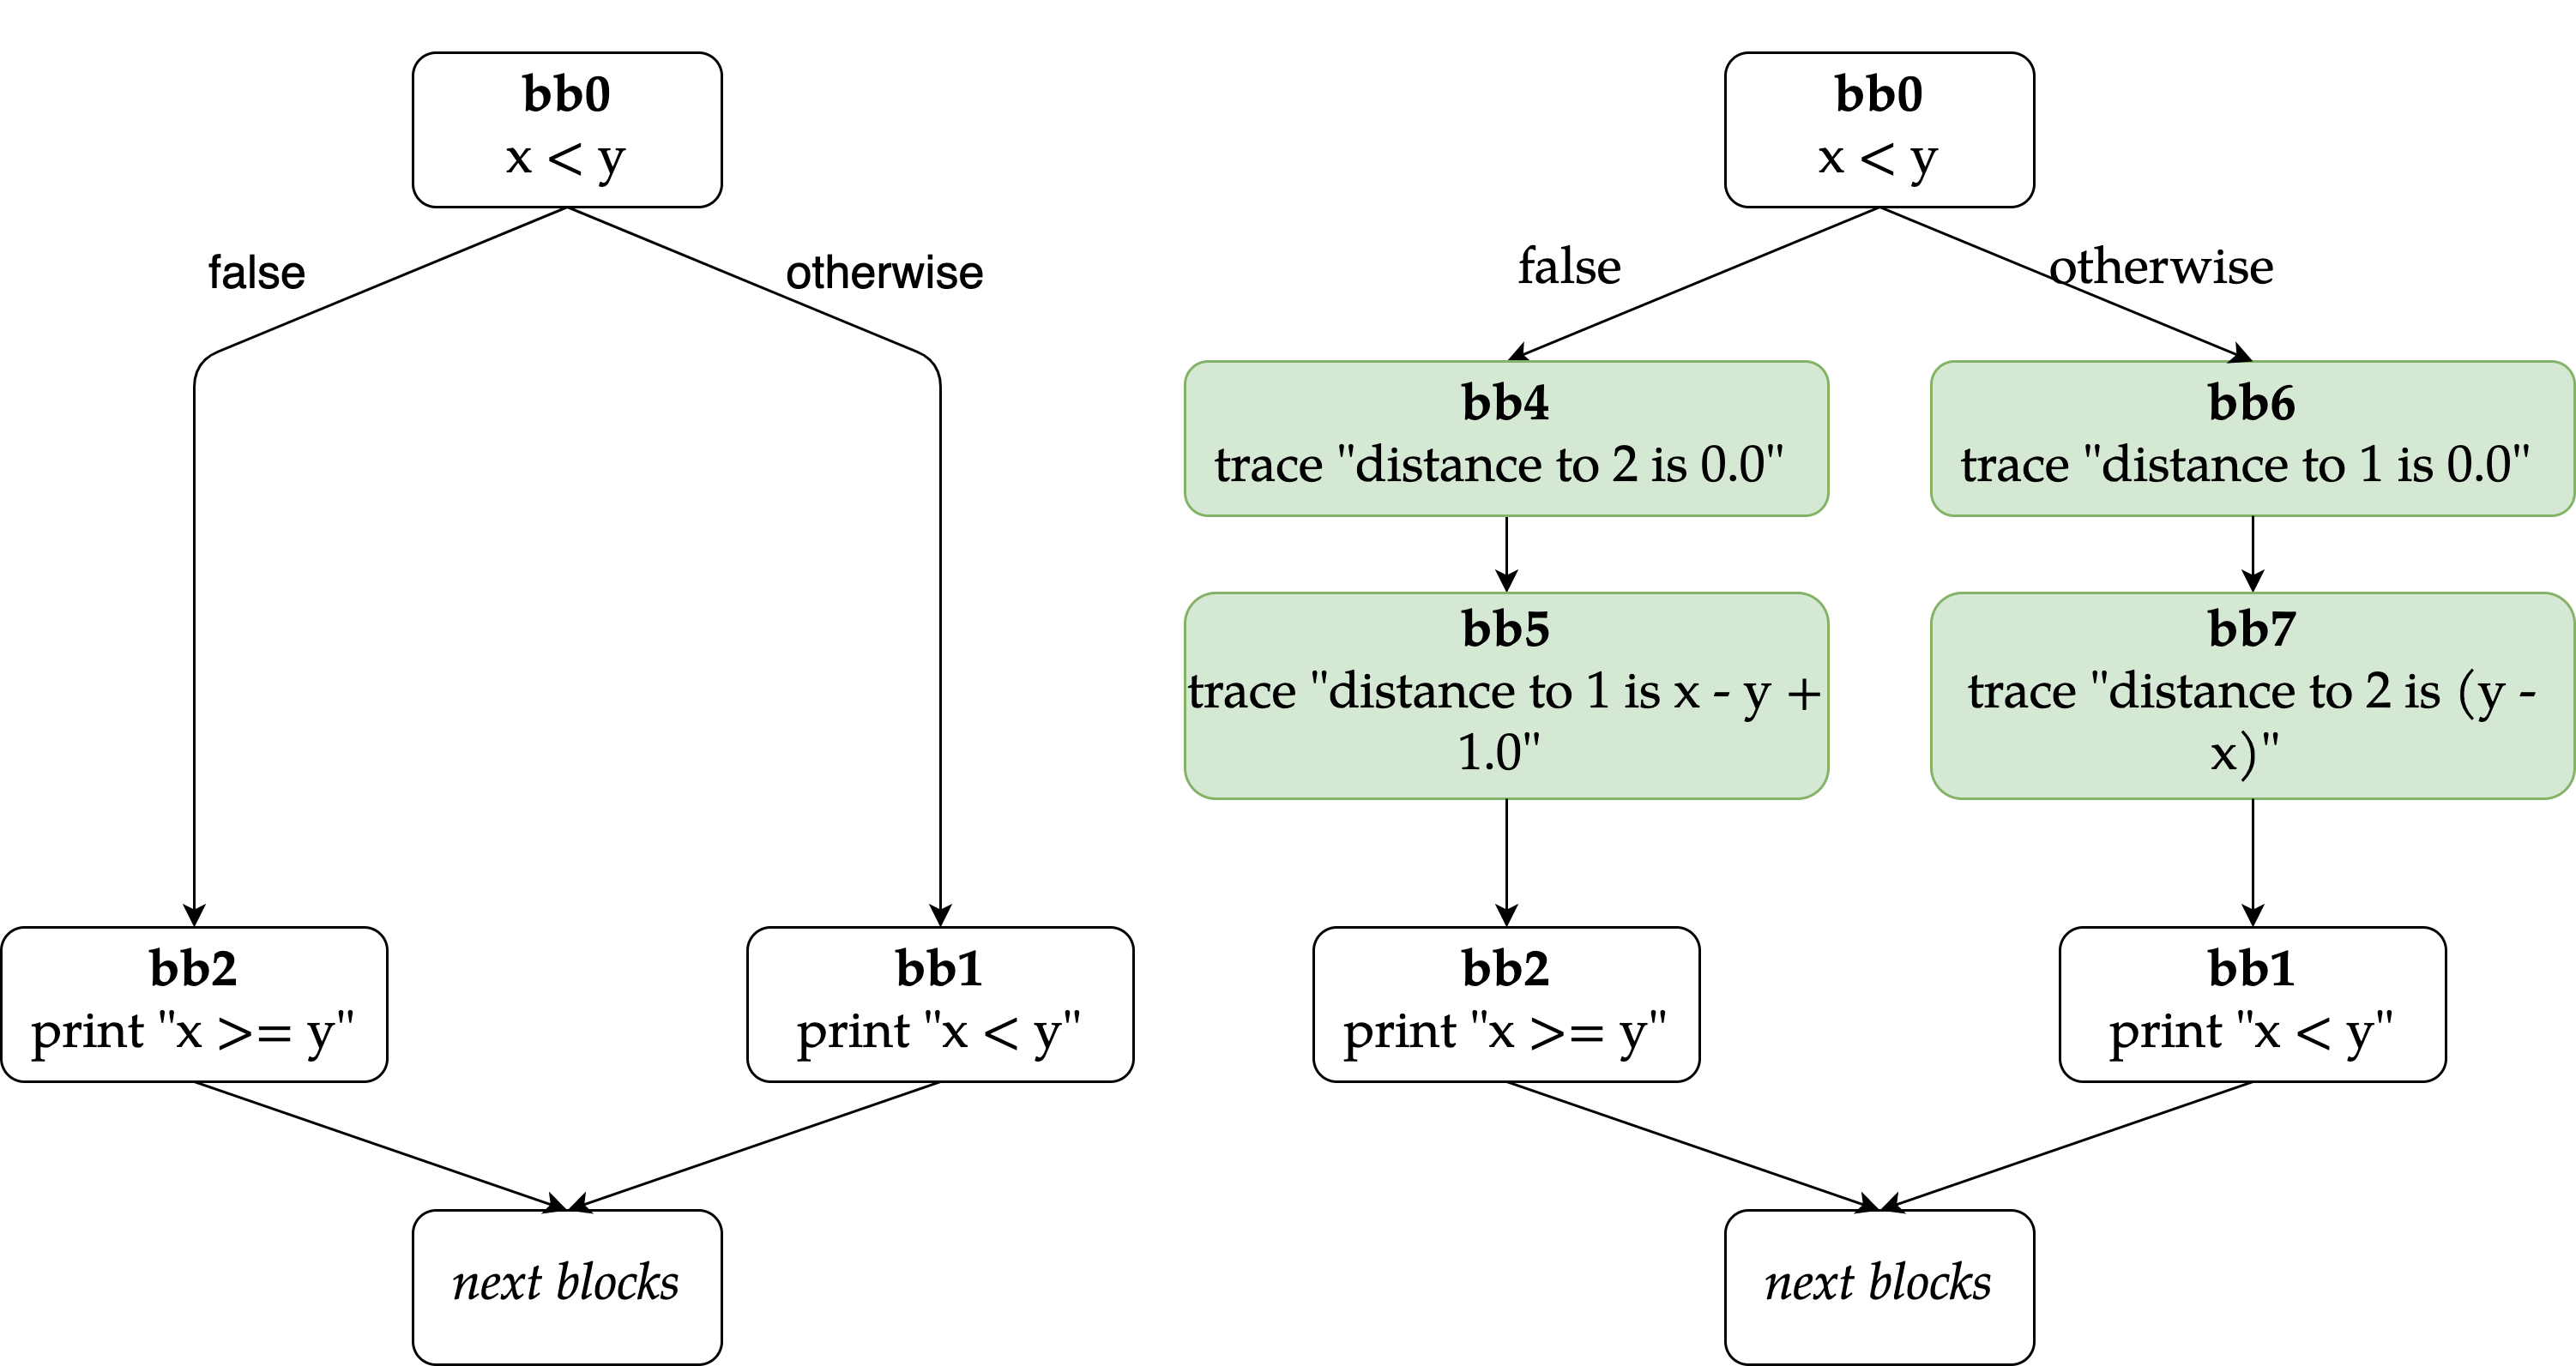
\includegraphics[width=\textwidth]{comparison-instrumented-branch-cfg}
\label{fig:comparison-instrumented-branch-cfg}
\end{figure}

\subsection{Testability Transformation Instrumentation}
\label{sec:mir-testability-transformations}
% TODO reword
In the following, we describe several transformations implemented in the \textsc{RustyUnit} test, some of which were presented by Fraser and Arcuri~\cite{Fraser2013} for the \textsc{EvoSuite} tool. The transformations are implemented at the \ac{MIR} level. To do this, we need to introduce more tracing blocks at crucial points. Basically, the Rust compiler transforms input programs in the same way as it is done with testability transformations, which are described in section 2. It inserts assertions at relevant places to check unexpected behavior, for example, whether an index is within array bounds or whether an arithmetic operation results in overflow or underflow.

For instance, when an arithmetic operation is accessed with an inappropriate index, the program will panic and crash. This happens because the compiler inserts checks before each array access and verifes whether the index is within the bounds of the array. Assume the following function that takes an index and an \texttt{i32} array and returns the value at the given position:
\begin{lstlisting}[style=boxed, caption={}, label=lst:array-index-access-example]
fn get(pos: usize, array: &[i32; 3]) -> i32 {
  array[pos]
}
\end{lstlisting}

The relevant part of it's \ac{MIR} looks like this:
\begin{lstlisting}[language={}, style=boxed, caption={}, label=lst:mir-boundary-check]
fn get(_1: usize, _2: &[i32; 3]) -> i32 {
  // Locals  definition

  bb0: {
    _3 = _1;
    _4 = const 3_usize;
    _5 = Lt(_3, _4);
    assert(move _5,
        "index out of bounds:
          the length is {} but the index is {}",
        move _4,
        _3) -> bb1;
  }

  bb1: {
    _0 = (*_2)[_3];
    return;
  }
}
\end{lstlisting}

That is, the compiler inserts an assertion that checks whether the index is less than the length of the array, which is statically constant. If the index is greater than or equal to the length, the program crashes. The other case, i.e. negative index, cannot occur since the index must always be of type \texttt{usize}, i.e. an unsigned type. Thus, there is no reason to verify this case.

Now, we need to insert tracing blocks for both, the ''good'' and the ''bad'' case. We could insert two branches always before an assertion block. However, in this case we would have to insert another branching block $s$, for example with \texttt{switchInt}, and if applicable we would have to change the original preceding assertion block so that it points to $s$. In the block $s$ we would also have to copy the logic from the assertion block, which makes the whole thing even more complicated. Another option would be to change the assertion itself. An assertion in \ac{MIR} has an optional unwind edge which, in the "bad" case, points to a sequence of blocks to clean up before the program crashes, if there is anything to clean up. Assume the function \texttt{get} from \Cref{lst:array-index-access-example} does some allocations before accessing the array:
\begin{lstlisting}[style=boxed, caption={}]
fn get(pos: usize, array: &[i32; 3]) -> i32 {
  let s = String::from("I'm using heap");
  array[pos]
}
\end{lstlisting}

Then, the the \ac{MIR} of the function becomes a bit different:
\begin{lstlisting}[language={}, style=boxed, caption={}, label=lst:mir-boundary-check-with-unwinding]
fn get(_1: usize, _2: &[i32; 3]) -> i32 {
  // Locals  definition
  bb0: {
    _3 = <String as From<&str>>::from(
      const "I'm using heap"
    ) -> bb1;
  }

  bb1: {
    _4 = _1;
    _5 = const 3_usize;
    _6 = Lt(_4, _5);
    assert(move _6,
      "index out of bounds:
        the length is {} but the index is {}",
      move _5,
      _4
    ) -> [success: bb2, unwind: bb4];
  }

  bb2: {
    _0 = (*_2)[_4];
    drop(_3) -> bb3;
  }

  bb3: {
      return;
  }

  bb4 (cleanup): {
    drop(_3) -> bb5; // drop the string
  }

  // Other blocks
}
\end{lstlisting}

The assertion has now got a second edge. Regardless of whether the index is valid or not, the string will be cleaned up in any case. The behavior is similar to the \texttt{finally} block from the \texttt{try-catch} construct in Java. Now we want to exploit the unwind edge of assertions. If an assertion has an unwind edge, we insert the tracing chain between the assertion and and the existing cleanup blocks. Otherwise, we create an unwind edge and connect it to the tracing chain. The instrumentation of assertions is illustrated in Figure~\Cref{fig:comparison-instrumented-assertion}. Since there are two branches, we also add a tracing chain of two tracing blocks to each branch. So in case the index is not valid, we trace the executed path normally before the program exits. Thus we know that the respective test has covered the path. In addition, we get a guidance for the two possible cases.

\begin{figure}[h]
\caption{Instrumented assertion}
\centering
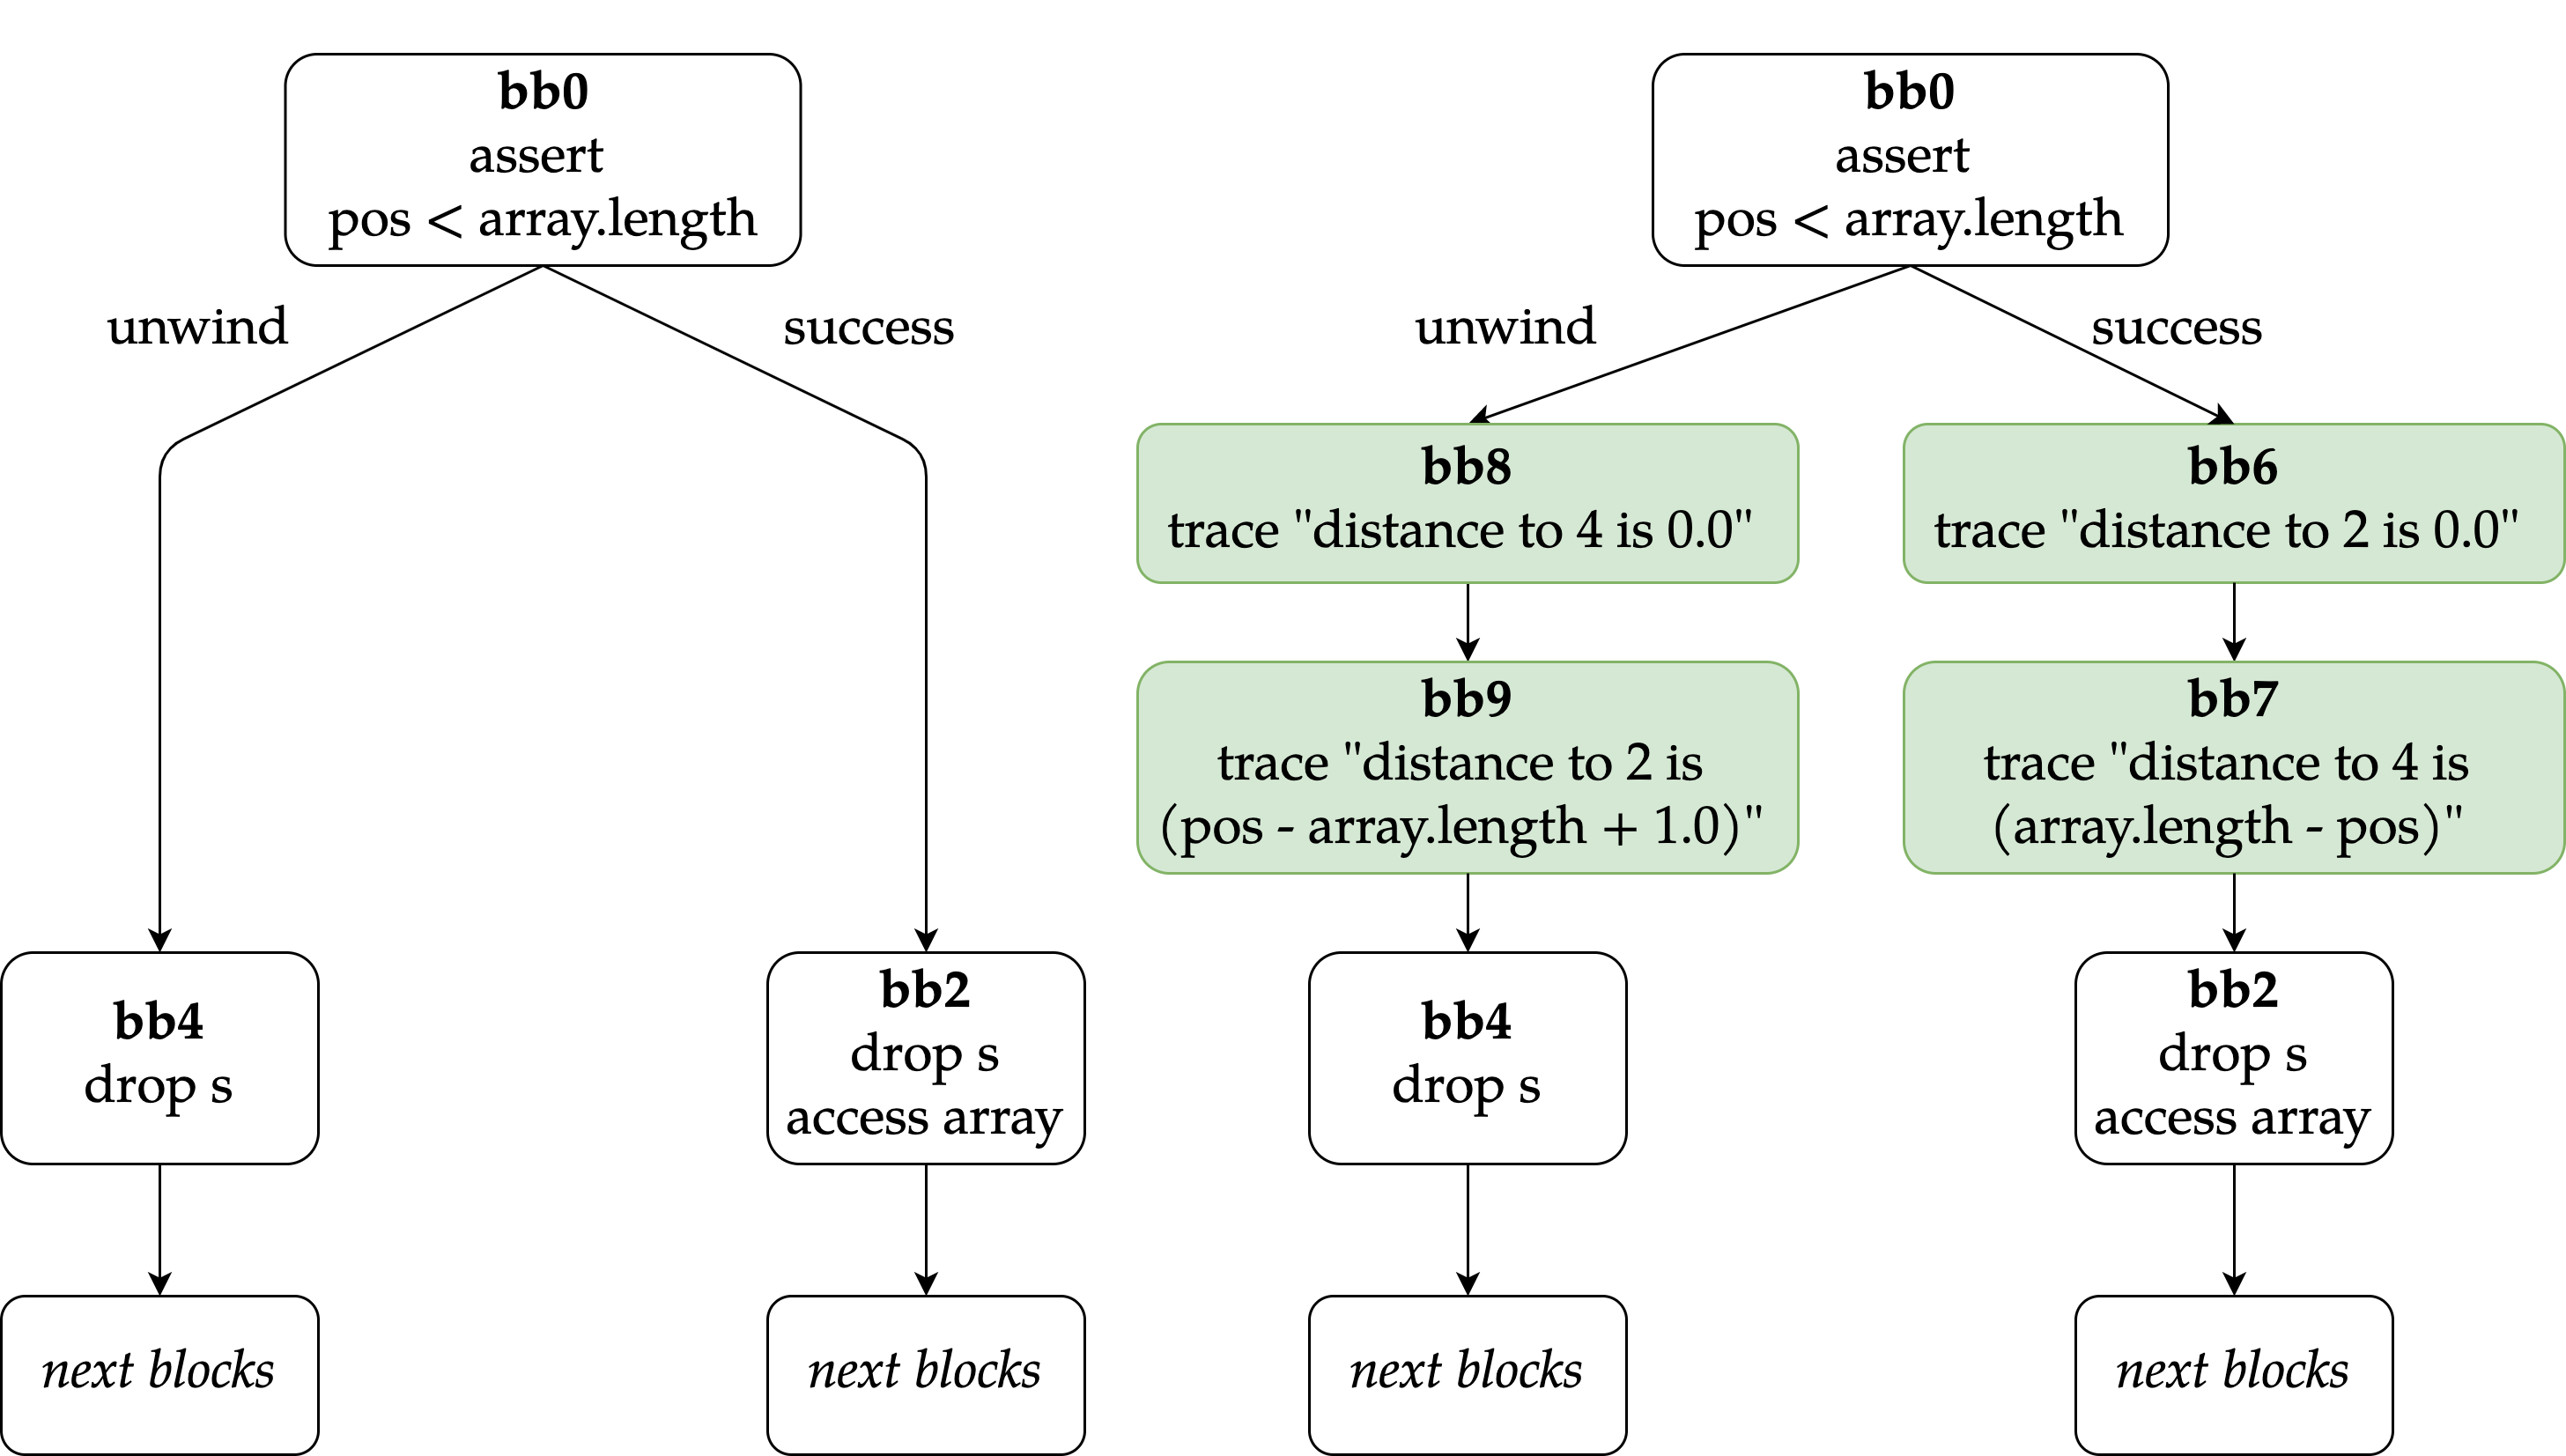
\includegraphics[width=\textwidth]{comparison-instrumented-assertion}
\label{fig:comparison-instrumented-assertion}
\end{figure}

We do the same for the case of overflows and underflows. \Cref{lst:mir-overflow-check} demonstrates an example of the \texttt{add} function that performs addition of two eight-bit integers and the relevant basic block from its \ac{MIR}. In the \ac{MIR}, the compiler inserts an assertion about the value of the result to catch an overflow. We instrument the assertion and insert our tracing chains into the body of the function as described above.
% OVERFLOW CHECK
\begin{lstlisting}[language={}, style=boxed, caption={\ac{MIR} overflow check}, label=lst:mir-overflow-check]
fn add(a: i8, b: i8) -> i8 {
  a + b
}

bb0: {
  _3 = _1;
  _4 = _2;
  _5 = CheckedAdd(_3, _4);
  assert(
    !move (_5.1: bool),
    "attempt to compute `{} + {}`,
      which would overflow",
    move _3,
    move _4
  ) -> bb1;
}
\end{lstlisting}

% \section{Test Construction}
% Kommt am 08.02.

% \subsection{Selection}
% Kommt am 08.02.

% \subsection{Crossover}
% Kommt am 08.02.

% \subsection{Mutation}
% Kommt am 09.02.


\section{Handling Generics and Traits}
A large part of \ac{SBST} approaches is applied to managed languages such as Java, since these offer a rich set of tools and features like reflection. It allows to analyze the code of the \ac{SUT} and extract information needed for generating tests by querying the appropriate language \ac{API}, like \texttt{getGenericParameters} of a \texttt{java.lang.reflect.Method} instance to get generic parameters. When tests are generated for generic elements, it is sometimes difficult to replace a generic type parameter with a matching concrete type because execution depends on the one concrete type~\cite{Fraser2014b}. As shown in \Cref{lst:java-isinstanceof}, an execution path for generic methods can be affected by checks for the concrete type of a generic instance. Many approaches to analyzing Java programs operate at the bytecode level after type erasure has already happened. This means that bytecode does not know anything about generics, they are replaced, for example, by \texttt{Object}.

\begin{lstlisting}[language=Java, style=boxed, caption={The execution path of the generic Java method depends on the concrete type of the argument}, label=lst:java-isinstanceof]
public class GenericsExample<T, K> {
  public int typedInput(T value) {
    if (value isinstanceof String) {
      return 0;
    } else if (value isinstanceof Integer) {
      return 1;
    } else if (value isinstanceof Double) {
      return 2;
    } else {
      return 3;
    }
  }
}
\end{lstlisting}

TODO

\begin{lstlisting}[style=boxed, caption={The execution path of the generic Rust function depends on the concrete type of the argument}, label=lst:rust-runtime-reflection]
use std::fmt::Debug;
use std::any::Any;

fn typed_input<T: Any>(value: &T) -> i32 {
  let value_any = value as &dyn Any;

  if let Some(as_string)
      = value_any.downcast_ref::<String>() {
    return 0;
  } else if let Some(as_int)
      = value_any.downcast_ref::<i32>() {
    return 1;
  } else if let Some(as_double)
      = value_any.downcast_ref::<f64>() {
    return 2;
  } else {
    return 3;
  }
}
\end{lstlisting}

% TODO reword
The problem of generics becomes relevant whenever the test generation algorithm attempts to instantiate a new instance of a generic type, or to satisfy a parameter for a newly inserted method call. Assume that our test generation algorithm decides to add a call to the method \texttt{new(bar: T)} of the struct \texttt{Foo<T>}, which is defined as follows:
\begin{lstlisting}[style=boxed, caption={}, label=lst:basic-generics-example]
struct Foo<T> {
    bar: T
}

impl<T> for Foo<T> {
    fn new(bar: T) -> Self {
        Self { bar }
    }

    fn update(&mut self, bar: T) {
        // ...
    }
}
\end{lstlisting}

% Aus der \ac{HIR} Analyse wissen wir, dass \texttt{T} ein Typparameter des Structs ist und durch keine weiteren Constraints gebunden ist. Das heißt, dass der Algorithmus in dem Fall einen beliebigen Typen statt \texttt{T} füllen kann. Um den Aufwand bei den Tests kleiner zu halten, prüfen wir immer zuerst, ob wir einen generischen Typparameter nicht durch einen primitiven Typ aus der Standard Library füllen können, sofern die Constraints dies erlauben. Hier würde sich der Algorithmus zum Beispiel für \texttt{isize} entscheiden. Somit würde folgender Methodenaufruf zum Test hinzugefügt:

From the \ac{HIR} analysis, we know that \texttt{T} is a type parameter of the struct and is not bound by any other constraints. This means that the algorithm can fill any type instead of \texttt{T} in that case. To keep the testing effort smaller, we always check first whether we cannot fill a generic type parameter by a primitive type from the standard library, if the constraints allow this. Here, for example, the algorithm would choose \texttt{isize}. Thus, the following method call would be added to the test:

\begin{lstlisting}[style=boxed, caption={}, label=lst:building-generic-test-1]
#[test]
fn rusty_test_0() {
    // ...
    let mut isize_0 = 42isize;
    let mut foo_0: Foo<isize> = Foo::new(isize_0);
    // ...
}
\end{lstlisting}

% Das Mapping \texttt|{T -> isize}| zwischen dem generischen Typparameter und dem konkreten Typ wird für die Variable für die spätere Nutzung gespeichert. So kann zum Beispiel ein weiterer Methodenaufruf, e.g., \texttt{update(&mut self, bar: T)}, auf der \texttt{Foo} Instanz generiert werden. Für den Aufruf muss erst das passende Argument generiert werden. Dabei ist bereits bekannt, dass die Variable \texttt{foo_0} den Typ \texttt{Foo<isize>} und somit das Mapping von \texttt{T} nach \texttt{isize} hat. Auf dieser Wissensbasis generiert der Algorithmus zwei weitere Statements wie folgt:

The mapping \texttt{\string{T -> isize\string}} between the generic type parameter and the concrete type is stored for the variable for later use. For example, another method call, e.g., \texttt{update(\string&mut self, bar: T)}, can be generated on the \texttt{Foo} instance. For the call, the appropriate argument must be generated first. It is already known that the variable \texttt{foo\string_0} has the type \texttt{Foo<isize>} and thus the mapping from \texttt{T} to \texttt{isize}. Using this knowledge base, the algorithm generates two more statements as follows:

\begin{lstlisting}[style=boxed, caption={}, label=lst:building-generic-test-2]
#[test]
fn rusty_test_0() {
  // ...
  let mut isize_0 = 42isize;
  let mut isize_1 = 145isize;
  let mut foo_0: Foo<isize> = Foo::new(isize_0);
  Foo::update(&mut foo_0, isize_1);
  // ...
}
\end{lstlisting}

% Generics Mixup Beispiel: https://doc.rust-lang.org/book/ch10-01-syntax.html

%Listing~\ref{lst:java-interface-example} shows the function \texttt{area} that accepts objects of type \texttt{Shape}, that is, instances of classes that implement the interface. To test the \texttt{area} function, one would have to find a type that implements the interface. Reflection can be used to query classes that do. This is possible because Java runs in a virtual machine that carries this information.

%\begin{lstlisting}[language=Java, style=boxed, caption={A function that takes objects implementing an interface}, label=lst:java-interface-example]
%public interface Shape {
%    double area();
%}
%
%public class Rectangle implements Shape {
%  private double length;
%  private double height;
%
%  @Override
%  public double area() {
%      return length * height;
%  }
%}
%
%public class Main {
%    public static double area(Shape shape) {
%        return shape.area();
%    }
%}
%\end{lstlisting}


Generics play an even greater role in Rust than in other object-oriented languages. More precisely, Rust is not a typical object-oriented language and instead of using direct types, for example as method parameters, as is often the case in Java, generics are rather used in conjunction with trait bounds. Trait bounds define what behavior a particular generic type must be capable of. This reduces the number of possible data types a type parameter can be filled with. \Cref{lst:trait-bounds-example} implements the \texttt{area} function in Rust, which takes a parameter of generic type~\texttt{T}. The type parameter \texttt{T} must implement the \texttt{HasArea} trait, which allows \texttt{area} to access the trait's functions. Unlike Java, there is no Reflection provided in Rust. Source code is compiled directly to machine executable code, and all superfluous information is eliminated during the compilation process.

\begin{lstlisting}[style=boxed, caption={A function that takes a generic types and specifies a bound}, label=lst:trait-bounds-example]
trait HasArea {
  fn area(&self) -> f64;
}

struct Rectangle { length: f64, height: f64 }

impl HasArea for Rectangle {
  fn area(&self) -> f64 { self.length * self.height }
}

// `T` must implement `HasArea`. Any type which meets
// the bound can access `HasArea`'s function `area`.
fn area<T: HasArea>(t: &T) -> f64 { t.area() }
\end{lstlisting}

Types that implement a particular trait must thus be found statically during compilation of the \ac{SUT} and annotated. The compiler provides \acp{API} to query all traits and the \texttt{impl} blocks, not only in the compiled \ac{SUT}, but also in its dependencies and in the standard library itself, as shown in \Cref{lst:query-types-that-implement-trait}.

\begin{lstlisting}[style=boxed, caption={Query types for a trait}, label=lst:query-types-that-implement-trait]
fn get_types_for_trait(trait_id: DefId, tcx: &TyCtxt<'_>) -> Vec<Type> {
  let trait_impls = tcx.trait_impls_of(trait_id);
  let types = trait_impls.iter()
    .map(|im| tcx.type_of(im))
    .collect::<Vec<_>>();

  // TODO substitue blanket implementations
}
\end{lstlisting}

Another difficulty is that traits themselves can be generic, as shown by the definition of \texttt{IntoIterator} from the standard library and its implementation from the \textbf{trying}~\footnote{\url{https://crates.io/crates/trying}} crate in \Cref{lst:intoiterator-trait}.

\begin{lstlisting}[style=boxed, caption={IntoIterator implementation in the \textbf{trying} crate}, label=lst:intoiterator-trait]
pub trait IntoIterator {
  type Item;
  type IntoIter: Iterator;
  fn into_iter(self) -> Self::IntoIter;
}

impl<A: TrieAtom, V: TrieValue> IntoIterator
  for Trie<A, V> {
  type Item = KeyValue<A, V>;
  type IntoIter = TrieIntoIterator<A, V>;

  fn into_iter(self) -> Self::IntoIter {
    // implementation ...
  }
}
\end{lstlisting}

However, finding all possible types implementing a particular trait which is not defined in the \ac{SUT} itself is difficult. Rust compiler proceeds similarly to C++ compiler when compiling: crates are compiled individually and independently and only then, for example, linked with the standard library. However, the \ac{SUT} from which the build process was started is always compiled last after all dependencies. Thus, all information is available at the time when \textsc{RustyUnit} performs the analysis. 

%Nevertheless, in order to provide certain implementations of traits when generating tests, we manually create several widely used type definitions as well as their methods and implemented traits. These definitions are automatically loaded and used by our tool. We define all primitive data types as well as several container types such as \texttt{std::vec::Vec}. \Cref{lst:vec-definition} shows the shortened definition of \texttt{std::vec::Vec}. Among other things, Vec implements the \texttt{IntoIterator} trait and thus could be used as an argument to test the \texttt{area} function from \Cref{lst:intoiterator-trait}. Moreover, it uses a generic type \texttt{T} which has no trait bounds. The method list is also provided so that the tool can create or modify an object of the respective type.

% \begin{lstlisting}[language={}, style=boxed, caption={std::vec::Vec type definition}, label=lst:vec-definition]
% name = std::vec::Vec
% generics = [(T, None)]
% traits = [std::iter::IntoIterator, ...]
% methods = [new() -> Self<T>, len(&self) -> usize, ...]
% \end{lstlisting}

In general, we mainly use primitive data types for a \ac{SUT} to keep the generated tests simple as far as this satisfies the defined trait bounds. To create a call to the example method \texttt{FooBar::foo} (\Cref{lst:generic-type-used-in-multiple-params}) in a generated test, we would do the following:

\begin{lstlisting}[style=boxed, caption={A generic type A is used in multiple parameters and return value}, label=lst:generic-type-used-in-multiple-params]
struct FooBar<A> { 
  // ...
}

impl<A> for FooBar<A> {
  fn new() -> Self {
    // ...
  }

  fn foo(&self, x: A, v: &Vec<A>) -> Option<A> {
    // ...
  }
}
\end{lstlisting}

\begin{enumerate}
    \item Look for a type that satisfies \texttt{A}; \texttt{A} has no bounds, so bind it to a primitive type, e.g., \texttt{i32}. Now, with that information, we know that the parameters \texttt{\string&self}, \texttt{x}, and \texttt{v} have to be of type \texttt{FooBar<i32>}, \texttt{i32}, and \texttt{Vec<i32>}, respectively.
    \item Using \texttt{GenObject} we find that an instance of \texttt{FooBar<A>} can be created by the constructor \texttt{FooBar::new()}, thus, we define \texttt{let f: FooBar<i32> = FooBar::new();}.
    \item Generating a primitive like \texttt{i32} is just a matter of defining some random value, like \texttt{let x: i32 = 42i32;}.
    \item Using \texttt{GenObject}, find a generator that returns a \texttt{Vec<i32>} or a \texttt{Vec<T>} with some generic type \texttt{T}.
    \item From our custom type definition, we know that \texttt{Vec::new()} returns a \texttt{Vec<T>}. We need its inner elements to be of type \texttt{i32}, which does satisfy the generic type \texttt{T}, so we take it and define \texttt{let v: Vec<i32> = Vec::new();}.
    \item Now, we can use the defined variables to generate a call to the \texttt{FooBar::foo} and store its returning value, whose bound type we are aware of, too, as shown in \Cref{lst:example-generated-test}.
\end{enumerate}

\begin{lstlisting}[style=boxed, caption={An example test that invokes \texttt{FooBar::foo}}, label=lst:example-generated-test]
#[test]
fn rusty_test_0() {
  let foobar_0: FooBar<i32> = FooBar::new();
  let i32_0: i32 = 42i32;
  let vec_0: Vec<i32> = Vec::new();
  let option_0: Option<i32> = FooBar::foo(
    &foobar_0, i32_0, &vec_0
  );
}
\end{lstlisting}

\clearpage
\chapter{Evaluation}
\label{chap:evaluation}
% TODO reword

We provide an empirical study on our search-based tool \textsc{RustyUnit} for automatic test case generation. We start by our reserch questions in \Cref{sec:research-questions}. Thereafter, we present our hypotheses we want to check during the evaluation in \Cref{sec:hypotheses}. Furthermore, we define the criteria for selecting case subjects for evaluation and present our case study in \Cref{sec:case-study-subjects} and explain the environment setup we used in \Cref{sec:environment-setup}. In \Cref{sec:results} we present the results and discuss them in \Cref{sec:discussion}. Finally, we conclude this chapter with a discussion of the threats to validity in \Cref{sec:threats-to-validity}.


\section{Research Questions}
\label{sec:research-questions}
% TODO reword
We now define questions that guide our evaluation. To determine how well our search-based approach performs with respect to code coverage and program crash detection, a set of experiments shall be conducted on a set of open-source Rust programs. As there is already another tool available, namely \textsc{KLEE}, which exploits \ac{DSE} and can also generate tests for Rust, we shall use it in the experiments and compare the results. \textsc{KLEE}-generated tests do not depend on the tool itself and can be executed outside of it the usual way. This opens the possibility to compute a source-based code coverage available in the Rust compiler for both tools. The experiments should answer the following questions:

%Symbolic execution often has problems constructing nice test suites with complex types, which is why this technique is rather applied to find bugs in a \ac{SUT}, than generate tests with high coverage. Seach-based approach do the opposite, they are good at generating tests with high coverage, but are not as good at finding bugs as they do not make use of test oracles~\cite{Fraser2013}.

\begin{enumerate}[start=1, label={\bfseries RQ\arabic*:}]
    \item How many coverage goals does \textsc{RustyUnit} cover?
    \item Does the \ac{GA} of \textsc{RustyUnit} achieve a better coverage than random search?
    \item Does \textsc{RustyUnit} generate less and shorter test cases than random search?
    \item Does \textsc{RustyUnit} achieve a higher code coverage than manually written tests in case study subjects?
    \item Does \textsc{RustyUnit} achieve a higher code coverage than the \ac{DSE}-based \textsc{KLEE}?
    \item How do the covered targets of \textsc{RustyUnit} and \textsc{KLEE} differ?
\end{enumerate} 


\section{Hypotheses}
\label{sec:hypotheses}
TODO Hier werden Hypothesen zur Evaluation beschrieben, die wir später mit Hilfe des nicht parametrisierten Mann-Whitney-U-Test jeweils für den Vergleich der Ergebnisse zwischen (random search und \textsc{RustyUnit}) und (\textsc{RustyUnit} und \textsc{KLEE}) überprüfen. Theoretisch wäre auch t-Test möglich, allerdings ist die Normalverteilung der Ergebnisse der such-basierten Testgeneierung nicht gegeben. Außerdem können wir keinen echten Mittelwert und Varianz bestimmen, da der Prozess theoretisch lange laufen könnte, sofern die 100\% Coverage nicht erreicht wird. Er ist praktisch durch die Rechen- und vor allem Speicherkapazität der Maschine begrenzt, was jedoch nur eine ''künstliche'' Grenze ist. Die Nullhypothese $H0$ wäre jeweils, dass sich die Performanz der Algorithmen nicht unterscheidet, bei $\alpha = 0.05$, wobei diese nicht so eine große Rolle spielt und man laut Arcuri~\cite{Arcuri2011} alle Ergebnisse unabhängig von der Signifikanz angeben und den Leser selbst entscheiden lassen sollte, inwieweit der jeweilige Algorithmus für ihn in Frage kommt. Statistische Auswertung und praktische, ''gefühlte'' Ergebnisse können sich bei randomisierten Algorithmen stark unterscheiden. 

Des Weiteren bestimmen wir jeweils die Effektgröße der Ergebnisse zwischen (random search und \textsc{RustyUnit}) und (\textsc{RustyUnit} und \textsc{KLEE}). Dazu nehmen wir den nicht parametrierten Vargha und Deleney's $\hat{A}_{12}$ Maßstab für die Effektgröße. Dessen Verwendung für randomisierte Algorithmen in Software Engineering wurde in~\cite{Leech2002} begründet und ein Beispiel dessen Verwendung im Kontext von Software Engineering mit randomisierten Algorithmen wird in~\cite{Poulding2010} gezeigt. 

\section{Case Study Subjects}
\label{sec:case-study-subjects}
For the evaluation, we randomly chose 15 open source crates from the Cargo's crate registry. This results in a total of 6661 methods.

\begin{table}[]
\begin{tabular*}{\textwidth}{l @{\extracolsep{\fill}} rrr}
\hline
\textbf{Case Study} & \textbf{\#Methods} & \textbf{\#Branches} & \textbf{LOC} \\
\hline
gamie & 116 &  & 328 \\
Pleco & 1188 &  & 6126 \\
time & 1158 &  & 5123 \\
url & 529 &  & 8822 \\
fixed & 370 &  & 3604 \\
ibig & 930 &  & 4859 \\
nom & 1375 &  & 3681 \\
thousands & 27 &  & 214 \\
trying & 104 &  & 408 \\
crc & 83 &  & 302 \\
rstar & 330 &  & 1085 \\
md5 & 24 &  & 150 \\
bytecount & 66 &  & 341 \\
PriorityQueue & 361 &  & 1173 \\
... & ... &  & ... \\
\hline
$\sum$ & 6661 & & 36216 \\
\hline
\end{tabular*}
\caption{\label{tab:properties-of-case-study-subjects}Number of methods, branches, and lines of code in the case study subjects}
\end{table}
% TODO reword
The libraries were chosen with respect to their testability. For experiments, it is necessary that the units are testable without complex interactions with external resources (e.g., databases, networks and filesystem) and are not multi-threaded. In fact, each experiment should be run in an independent way, and there might be issues if automatically generated test cases do not properly de-allocate resources. Notice that this is a problem common to practically all automated testing techniques in the literature. \Cref{tab:properties-of-case-study-subjects} summarizes the properties of these case study subjects in terms of the number of methods, branches, and lines of code. We calculated these metrics using Mozilla's rust-code-analysis tool~\cite{Ardito2020}. By ''methods'' is meant the total number of methods, functions, and closures. Lines of code means the number of logical lines, i.e. statements, in the respective crate as specified by the \textit{LLOC} metric in rust-code-analysis.

% Specifically, we picked the following crates:
% \begin{itemize}
%     \item \textit{trying (v0.1.0)}\footnote{\url{https://crates.io/crates/trying/}}, a simple Trie implementation for storing ''keys'' composed of ''atoms'',
%     \item \textit{num-iter (v0.1.42)}\footnote{\url{https://crates.io/crates/num-iter/}}, generic Range iterators for Rust,
%     \item \textit{num (v0.4.0)}\footnote{\url{https://crates.io/crates/num}}, a collection of numeric types and traits for Rust,
%     \item \textit{crc (v2.1.0)}\footnote{\url{https://crates.io/crates/crc}}, a Rust implementation of CRC(8, 16, 32, 64),
%     \item \textit{rstar (v0.9.2)}\footnote{\url{https://crates.io/crates/rstar}}, a flexible, n-dimensional r*-tree implementation,
%     \item \textit{md5 (v0.7.0)}\footnote{\url{https://crates.io/crates/md5}}, a MD5 hash function implementation,
%     \item \textit{bytecount (v0.6.2)}\footnote{\url{https://crates.io/crates/bytecount}}, a byte counting crate,
%     \item \textit{PriorityQueue (v1.2.1)}\footnote{\url{https://crates.io/crates/priority-queue}}, a priority queue with a function to change the priority of an object.
% \end{itemize}

\section{Setup}
\label{sec:environment-setup}
% TODO reword
As witnessed in \Cref{sec:search-operators}, search algorithms are influenced by a great number of parameters. For many of these there are ''best practices''. We chose many of them based on the experience of other search-based tools like \textsc{EvoSuite}~\cite{Fraser_2011a} and \textsc{Pynguin}~\cite{Lukasczyk2020}. Altough longer test cases are better in general, we limited the length of test cases to $L = 80$ because we experienced this to be a suitable length at which the test case execution does not take too long, altough the initial test cases are generated with only $10$ statements each. The population size for the \ac{GA} was chosen to be $80$.

Search algorithms are often compared in terms of the number of fitness evaluations or generated chromosome samples. That is, the algorithms used in the evaluation have the same budget of generated chromosomes and the performance of the algorithms is compared using the code coverage of test cases that remain after the algorithms have used up the budget. This is what we use to compare \textsc{RustyUnit} with random search. As discussed by Ali et al.~\cite{Ali2010}, a search algorithm should always be compared against at least random search in order to check that the algorithm is not simply successful because the search problem is easy. For evaluation, we have included the option of a random search, which generates random test cases in a manner similar to the initial population in the genetic algorithm of \textsc{RustyUnit}. The random search also uses an archive and stores test cases that execute previously uncovered branches in \ac{SUT}. The random search uses the same parameters for maximum test length, population size, and any probabilities as are set for \textsc{RustyUnit}. The intuition is that the \ac{GA} of \textsc{RustyUnit} will at least provide better test cases in terms of code coverage, since the basis for generation is the same, but the \ac{GA} of \textsc{RustyUnit} has a lead.

% Den Vergleich von \textsc{RustyUnit} \ac{GA} mit dem \ac{DSE}-basierten Tool KLEE können wir nicht anhand der Anzahl von generierten Chromosomen durchziehen, da \ac{DSE} Algorithmen keine Chromosome generieren und somit nicht die Evaluation der Fitness durchführen. Das einzige adäquate Kriterium ist in diesem Fall die Zeit. Das heißt, dass beide Algorithmen, dass die Suche entweder nach dem Finden einer Lösung mit 100\% Coverage oder nach dem Ablaufen einer bestimmten Zeit. \acp{GA} besitzen die Eigenschaft, dass sie zu jedem Zeitpunkt ihrer Ausführung eine Sammlung von bereits gefundenen Test Cases haben, sodass ein Abbruch nach einem gewissen Zeitlimit trotzdem handhabbare Ergebnisse haben kann. Ob das für \ac{DSE} ebenso der Fall ist, bezweifeln wir hier etwas. Wenn nicht, dann heißt das, dass das Zeitbudget maßgeblich von der Ausführungszeit von KLEE bestimmt wird. Nach dem das Tool fertig wird, können wir \textsc{RustyUnit} ebenfalls stoppen.

The comparison of \textsc{RustyUnit} \ac{GA} with the \ac{DSE}-based tool \textsc{KLEE} cannot be carried through based on the number of chromosomes generated, since \ac{DSE} algorithms do not generate chromosomes and thus do not perform fitness evaluation. The only adequate criterion in this case is time. That is, both algorithms that search either after finding a solution with $100\%$ coverage or after a certain time has elapsed. \acp{GA} have the property that they have a collection of already found test cases at any point in their execution, so stopping after a certain time limit can still have manageable results. Whether this is equally the case for \ac{DSE}, we somewhat doubt here. If not, it means that the time budget is largely determined by the execution time of \textsc{KLEE}. After the tool finishes, we can stop \textsc{RustyUnit} as well.

% Um die Performanz der Algorithmen zu messen, wird bei der Evaluation der generierten Test Cases die sogenannte \textit{instrument-coverage} des Rust Compilers verwendet. Rust unterstützt eigentlich zwei Coverage-Arten. Zum einen, die \textit{gcov}, die die Debug Information verwendet, um von LLVM IR nach Quellcode zu mappen. Dabei wird die LLVM IR instrumentiert, um die ausgeführten Befehle zu zählen. Da LLVM jedoch nichts von der Codesturktur von Rust weiß, gehen auf diese Weise viele Details verloren und die gemessene Coverage ist nur eine Annäherung an die tatsächliche Coverage, was nur mittelmäßig gut ist. Zum anderen unterstützen die neueren Versionen des Rust Compilers die Quellcode-basierte Coverage, auch genannt \textit{instrument-coverage}. Hierbei wird Rust Code (seine MIR, um genau zu sein) direkt instrumentiert, bevor er in die LLVM IR umgewandelt wird. Da die MIR ein Mapping zwischen Quellcode und dem CFG eines Programms ist, können selbst Stellen wie short-circuited conditionals, closures, and match guards präzise abgebildet werden.

To measure the performance of the algorithms, the so-called \textit{instrument-coverage} of the Rust compiler is used when evaluating the generated test cases. Rust actually supports two types of coverage. For one, the \textit{gcov}, which uses the debug information to map from LLVM \ac{IR} to source code. In this case, the LLVM \ac{IR} is instrumented to count the executed instructions. However, since LLVM does not know anything about Rust's code structure, a lot of details are lost this way and the measured coverage is only an approximation of the actual coverage, which is only moderately good. On the other hand, the newer versions of the Rust compiler support source code based coverage, also called \textit{instrument-coverage}. Here, some Rust code (its \ac{MIR}, to be precise) is instrumented directly before being converted to the LLVM \ac{IR}. Since the \ac{MIR} is a mapping between source code and the \ac{CFG} of a program, even places like short-circuited conditionals, closures, and match guards can be accurately mapped.

% Damit die \textit{instrument-coverage}~\footnote{\url{https://doc.rust-lang.org/stable/unstable-book/compiler-flags/instrument-coverage.html}} benutzt werden kann, muss das SUT mit dem entsprechenden Flag \texttt{-Z instrument-coverage} kompiliert werden. Hierbei wird eine \textit{profiler runtime} benötigt, die im \textit{nightly} Compiler bereits mit dabei ist. Somit wird ein entsprechendes SUT mit \raggedright\texttt{RUSTFLAGS="-Z instrument-coverage" cargo +nightly build} gebaut. Bei der Ausführung des gebauten Programs bzw. Tests werden von LLVM entsprechende Coverage (\texttt{profdata}) Dateien generiert, die nach dem Postprocessing die Line- sowie Branchcoverage per Quellcode-Datei des SUT enthalten. Für jeden der drei Algorithmen vergleichen wir die Line- und Branch-Coverage, sowie die Länge und Anzahl der generierten Tests. Da beide Tools, \textit{KLEE} und \textit{RustyUnit}, Tests in Quellcode-Form generiert werden, können sie zusammen mit dem SUT kompiliert und ihre Quellcode-basierte Coverage direkt verglichen werden.

In order to use the \textit{instrument-coverage}~\footnote{\url{https://doc.rust-lang.org/stable/unstable-book/compiler-flags/instrument-coverage.html}} the SUT must be compiled with the corresponding flag \texttt{-Z instrument-coverage}. This requires a \textit{profiler runtime}, which is already included in the \textit{nightly} compiler. Thus a corresponding SUT is built with \raggedright\texttt{RUSTFLAGS="-Z instrument-coverage" cargo +nightly build}. When the built program or test is executed, LLVM generates corresponding coverage (\texttt{profdata}) files, which after post-processing contain the line as well as branch coverage per source file of the \ac{SUT}. For each of the three algorithms, we compare the line and branch coverage, as well as the length and number of generated tests. Since both tools, \textsc{KLEE} and \textsc{RustyUnit}, generate tests in source code form, they can be compiled along with the \ac{SUT} and their source code-based coverage can be directly compared.

\textsc{RustyUnit} and search-based testing relies on randomized algorithms, which are inherently affected by chance. Running a randomized algorithm twice will most likely produce different results. It is essential to use rigorous statistical methods to properly analyze the performance of randomized algorithms when we need to compare two or more of them. In this work, we follow the guidelines described by Arcuri and Briand~\cite{Arcuri2011}. Since comparisons with simpler alternatives (at a very minimimum random search) is a necessity when one proposes a novel randomized algorithm or addresses a new software engineering problem~\cite{Ali2010}, statistical testing should be part of the according work, which reports such empirical study. For each of the 14 crates, we ran \textsc{RustyUnit} against the random search and \textsc{KLEE} to compare their achieved code coverage. Each experiment comparison was repeated ...? times (~\cite{Arcuri2011} schlägt mindestens $1000$ vor, bei begründet langer Ausführungszeit kann es auch weniger sein) with different seeds for the random number generator.

\section{Results}
\label{sec:results}
% TODO reword
In the following we analyse the benchmark results in order to answer our research questions and test our hypotheses. 

\subsection{Coverage Goals in Evaluation Subjects}

TODO 
% RQ 1 answer
\begin{tcolorbox}
\textbf{Summary (RQ1):} \textsc{RustyUnit} covers $n$ out of $m$ coverage goals on average.  
\end{tcolorbox}

\subsection{Failing Tests}
TODO 

Figure ... lists the failures found in each of the case study subject by \textsc{RustyUnit}. 

\subsection{Comparison with Random Search}
Statistical difference has been measured with the Mann-Whitney U test. To quantify the improvement in a standadized way, we used the Vargha-Delaney~$\hat{A}_{12}$ effect size. In our context, the $\hat{A}_{12}$ is an estimation of the probability that, if we run \textsc{RustyUnit}, we will obtain better coverage than running the random search strategy. When two randomized algorithms are equivalent, then $\hat{A}_{12} = 0.5$. A high value $\hat{A}_{12} = 1$ means that, in \textit{all} of the $100$ runs of \textsc{RustyUnit}, we obtained coverage values higher than the ones obtained in \textit{all} of the $100$ runs of the random search strategy.

\begin{table}[]
\begin{tabular*}{\textwidth}{l @{\extracolsep{\fill}} rrr}
\hline
\textbf{Case Study} & \textbf{$\hat{A}_{12} < 0.5$} & \textbf{$\hat{A}_{12} = 0.5$} & \textbf{$\hat{A}_{12} > 0.5$} \\
\hline
gamie &  &  &  \\
Pleco &  &  &  \\
time &  &  &  \\
url &  &  &  \\
fixed &  &  &  \\
ibig &  &  &  \\
nom &  &  &  \\
thousands &  &  &  \\
trying &  &  &  \\
crc &  &  &  \\
rstar &  &  &  \\
md5 &  &  &  \\
bytecount &  &  &  \\
PriorityQueue &  &  &  \\
... & ... &  & ... \\
\hline
$\sum$ &  & &  \\
\hline
\end{tabular*}
% TODO reword caption
\caption{\label{tab:results-ru-rs-coverage}$\hat{A}_{12}$ measure values in the coverage comparisons: $\hat{A}_{12} < 0.5$ means \textsc{RustyUnit} resulted in less, $\hat{A}_{12} = 0.5$ equal, and $\hat{A}_{12} > 0.5$ better coverage than a random search approach}
\end{table}

The box-plot in Figure ... compares the actual obtained coverage values (averaged out of the $100$ runs) of \textsc{RustyUnit} and the random search strategy. In total, the coverage improvement ...

TODO das mit den Farben funktioniert nicht so richtig :/
\begin{tikzpicture}
  %\caption{\label{fig:results-ru-rs-coverage} Comparison of statement coverage between \textsc{RustyUnit} and random search}
  \begin{axis}
    [ 
      ylabel={Coverage (\%)},
      boxplot/draw direction=y,
      boxplot/variable width,
      boxplot/every box/.style={fill=gray!50},
      cycle list={{thesisblue},{codegray}},
      boxplot={
        draw position={1/3 + floor(\plotnumofactualtype/2) + 1/3*mod(\plotnumofactualtype,2)},
        box extend=0.3,
      },
      x=2cm,
      xtick={0,1,2,...,10},
      x tick label as interval,
      xticklabels={%
        {gamie},%
        {Pleco},%
        {time},%
        {url},%
      },
      x tick label style={
        text width=2.5cm,
        align=center
      },
      %every axis plot/.append style={fill,fill opacity=0.5},
      %every axis plot/.append style={fill,fill opacity=0.5}
    ]

  % gamie
  \addplot[boxplot] table[row sep=\\,y index=0] {
    0.55 \\ 
    0.48 \\ 
    0.55 \\ 
    0.60 \\ 
    0.65 \\ 
    0.53 \\ 
    0.30 \\
  };
  \addplot[boxplot] table[row sep=\\,y index=0] {
    0.3 \\ 
    0.26 \\ 
    0.35 \\ 
    0.45 \\ 
    0.38 \\ 
    0.45 \\ 
    0.24 \\ 
  };

  % Pleco
  \addplot[boxplot] table[row sep=\\,y index=0] {
    0.55 \\ 
    0.38 \\ 
    0.42 \\ 
    0.50 \\ 
    0.48 \\ 
    0.43 \\ 
    0.50 \\  
  };
  \addplot[boxplot] table[row sep=\\,y index=0] {
    0.35 \\ 
    0.38 \\ 
    0.30 \\ 
    0.18 \\ 
    0.25 \\ 
    0.30 \\ 
    0.25 \\ 
  };

  % time
  \addplot[boxplot] table[row sep=\\,y index=0] {
    0.46 \\ 
    0.48 \\ 
    0.45 \\ 
    0.55 \\ 
    0.30 \\ 
    0.55 \\ 
    0.45 \\
  };
  \addplot[boxplot] table[row sep=\\,y index=0] {
    0.30 \\ 
    0.27 \\ 
    0.35 \\ 
    0.32 \\ 
    0.35 \\ 
    0.24 \\ 
    0.25 \\
  };

  % url
  \addplot[boxplot] table[row sep=\\,y index=0] {
    0.40 \\ 
    0.48 \\ 
    0.44 \\ 
    0.55 \\ 
    0.45 \\ 
    0.43 \\ 
    0.34 \\
  };
  \addplot[boxplot] table[row sep=\\,y index=0] {
    0.30 \\ 
    0.35 \\ 
    0.15 \\ 
    0.28 \\ 
    0.32 \\ 
    0.23 \\ 
    0.3 \\ 
  };
  \end{axis}
\end{tikzpicture}

% RQ 2 answer
\begin{tcolorbox}
\textbf{Summary (RQ2):} \textsc{RustyUnit} \textbf{(hopefully)} achieves \textbf{higher coverage} than random search test case generation. 
\end{tcolorbox}

\subsection{Manually written tests}

\subsection{Comparison with DSE}

\section{Threats to Validity}
\label{sec:threats-to-validity}
Die in der Evaluation verwendeten Crates sind eher klein gehalten und vor allem so, dass sie möglichst wenige Dependencies haben, d. h. in sich geschlossen bleiben. Sie interagieren nicht mit der Umgebung, z. B. mittels I/O, und wodurch die Ergebnisse nicht auf alle möglichen Rust Programme generalisiert werden können. Außerdem wird hier teilweise ein wichtiges Feature von Rust außer Acht gelassen: Die Codegenerierung mittels Makros. Der zur Kompilierzeit generierte Code, wie beispielsweise vom \texttt{serde} Crate, stellt unter anderem Schwierigkeiten durch seine Komplexität dar, die einen extensiven Zeitaufwand benötigt. Des Weiteren werdem hier keine Multithreaded Programme behandelt. Streng genommen sind die hier generierten Tests nicht ganz Unit Tests, da sie unter anderem auf modulfremde Implementierungen zugreifen, um Argumente für einen bestimmten Methodaufruf zu generieren. Das wird normalerweise mittels Mocks gehandhabt (zum Beispiel mit Hilfe des Mockito~\footnote{\url{https://site.mockito.org/}} Framework für Java). Leider funktioniert das in Rust bis jetzt nur mäßig gut, da Mocks nur für Traits gut funktionieren, jedoch nicht für konkrete Structs. 

Moreover, bei den generierten Tests möchte man unter anderem wissen, ob zwei Tests eigentlich equal und dadurch teilweise überflüssig sind, allerdings ist das ein ganz anderes Problem. Somit generieren wir einfach einen Haufen von Tests und hoffen auf das Beste. Um den Rest soll sich jemand in Future kümmern.

MIR ist nicht stabil und kann sich in zukünftigen Versionen ändern, sodass die Implementierung nicht mehr zusammenpasst.

% \section{Code Coverage Comparison with Manually Written Tests}
% \begin{table}[]
% \begin{tabular*}{\textwidth}{l @{\extracolsep{\fill}} cccc}
% \hline
% \textbf{Crate} & \textbf{120s} & \textbf{240s} & \textbf{360s} & \textbf{480s} \\ \hline
% trying         &       -       &       -        &        -         &       -       \\
% num-iter       &       -       &       -        &        -         &       -       \\
% num            &       -       &       -        &        -         &       -       \\
% crc            &       -       &       -        &        -         &       -       \\
% rstar          &       -       &       -        &        -         &       -       \\
% md5            &       -       &       -        &        -         &       -       \\
% bytecount      &       -       &       -        &        -         &       -       \\
% PriorityQueue  &       -       &       -        &        -         &       -       \\ \hline
% \end{tabular*}
% \caption{Detailed results of \textsc{RustyUnit} on the branch coverage}
% \end{table}


% \begin{table}[]
% \begin{tabular*}{\textwidth}{l @{\extracolsep{\fill}} ccccc}
% \hline
% \textbf{Crate} & \textbf{Budget time} & \textbf{Min} & \textbf{Mean} & \textbf{Median} & \textbf{Max} \\ \hline
% trying         &       -       &      -       &        -        &       -   &       -   \\
% num-iter       &       -      &       -        &        -         &       -    &       -    \\
% num            &       -      &       -        &        -         &       -    &       -    \\
% crc            &       -      &       -       &        -         &       -   &       -    \\
% rstar          &       -      &       -       &        -       &       -   &       -    \\
% md5            &       -      &       -       &        -        &       -    &       -   \\
% bytecount      &       -      &       -        &        -         &       -   &       -    \\
% PriorityQueue  &       -      &       -        &        -         &       -  &       -    \\ \hline
% \end{tabular*}
% \caption{Statistics about generated tests}
% \end{table}
% \section{Code Coverage Comparison with \textsc{KLEE}}

\section{Conclusion}
\label{sec:discussion}

\clearpage
\chapter{Future Work}
\label{chap:future-work}
% TODO reword
Solving a research problem almost always leads to new problems and further open questions. In this final section of the thesis, we want to discuss a few such questions that arose during the work on the thesis. We leave them as future work because they would blast the scope of this work. 

We already stated in the evaluation that the whole process of generating tests for Rust with \textsc{RustyUnit} is relatively slow and cannot be applied easily to all crates of any size out in the wild. The execution time is very tied to the execution of the Rust compiler and I/O operations, which means that the cost of the runtime of the generated tests themselves is not the bottleneck. At this point, cache optimizations could be made or the way \ac{SUT} is instrumented and tests are executed could be adjusted. Furthermore, the generated tests contain a lot of unnecessary statements, which would lead to the running, but more importantly comprehension overhead of a humble developer who would have to deal with them, since the tests do not use automatic oracles like assertions. This leads us to the other aspect of test generation: \textsc{RustyUnit} does not generate real test cases, but only program executions. A test oracle, which determines whether the result of an execution is correct and meets the expectations, is missing. Some test generation tools, such as \textsc{EvoSuite}, can automatically incorporate assertions, for example by using the recorded behavior of \ac{SUT} for regression testing. In the future, a mechanism for automatically generated oracles could also be provided in \textsc{RustyUnit}.

Another aspect of test generation is the scope of the test cases. Unit testing, as the name suggests, refers to individual units. Traditionally, complex dependencies are replaced by mocks in unit tests, e.g., a database connection. As far as possible, \textsc{RustyUnit} exploits real data types, even if they come from other units, which makes it more an integration test suite generator. Rust's ecosystem already offers many mock libraries, but unlike Java, they do not rely on reflection, but on Rust's strong macro system and generate mocks at compile time. It would be interesting to extend \textsc{RustyUnit}'s search-based algorithm with functional mocks to achieve potentially better coverage, such as Arcuri et al.~\cite{Arcuri2017} do for \textsc{EvoSuite}.

Finally, it would be useful to use Rust's compiler analysis for more meaningful tests. \textsc{RustyUnit} is a compiler wrapper and can thus access all compiler internals during the analysis of the \ac{SUT}. Advanced static analysis of the \ac{SUT}, such as backwards search of the definitions of operands in conditions, could help generate better tests with higher coverage. 


\backmatter% Now we are in the appendix
\appendix
\cleardoublepage
\thispagestyle{empty}
\null\vfill
\noindent\textbf{Eidesstattliche Erklärung:}\\[1.5ex]
Hiermit versichere ich an Eides statt, daß ich diese Bachelorarbeit
selbstständig und ohne Benutzung anderer als der angegebenen Quellen und
Hilfsmittel angefertigt habe und daß alle Ausführungen, die wörtlich oder
sinngemäß übernommen wurden, als solche gekennzeichnet sind, sowie daß ich die
Bachelorarbeit in gleicher oder ähnlicher Form noch keiner anderen
Prüfungsbehörde vorgelegt habe.\\[1.5cm]
Place, \today\quad\rule{6cm}{0.1mm}\\
\null\hspace{5cm} {\small Thesis Author}

\clearpage
\chapter{Acronyms}
\begin{acronym}
	\acro{SUT}{System Under Test}
	\acro{CUT}{Class Under Test}
	\acro{MUT}{Method Under Test}
	\acro{SMT}{Satisfiability Modulo Theories}
	\acro{GA}{Genetic Algorithm}
	\acro{EA}{Evolutionary Algorithm}
	\acro{MOSA}{Many-Objective Sorting Algorithm}
	\acro{DynaMOSA}{Many-Objective Sorting Algorithm with Dynamic target selection}
	\acro{WS}{Whole Suite}
	\acro{WSA}{Whole Suite with Archive}
	\acro{SBST}{Search-based Software Testing}
	\acro{SBSE}{Search-based Software Engineering}
	\acro{ATP}{Automated Theorem Prover}
	\acro{DSE}{Dynamic Symbolic Execution}
	\acro{IR}{Intermediate Representation}
	\acro{MOA}{Multi- and Many-Objective Algorithm}
	\acro{DDG}{Data Dependence Graph}
	\acro{HIR}{High-level Intermediate Representation}
	\acro{THIR}{Typed HIR}
	\acro{MIR}{Mid-level Intermediate Representation}
	\acro{AST}{Abstract Syntax Tree}
	\acro{CFG}{Control Flow Graph}
	\acro{CDG}{Control Dependence Graph}
	\acro{API}{Application Programming Interface}
	\acro{NSGA-II}{Non-dominated Sorting Genetic Algorithm II}
	\acro{TCP}{Transmission Control Protocol}
	\acro{SSA}{Static Single Assignment}
\end{acronym}

\clearpage
\printbibliography
\end{document}
